%&LaTeX
% !TEX encoding = UTF-8 Unicode
\documentclass{report}
\usepackage[utf8]{inputenc}
\usepackage[T1]{fontenc}
\usepackage{textcomp}
\usepackage{float,fancyvrb}
\usepackage{listings}
\usepackage{xspace}

%\usepackage{graphicx}
\usepackage{longtable}
\usepackage{color}

\usepackage{ifpdf}

\ifx\pdftexversion\undefined %if using TeX
    \usepackage{graphicx}
\else %if using PDFTeX
    \ifpdf %if using PDFTeX in PDF mode
        \usepackage[pdftex]{graphicx}
        \DeclareGraphicsExtensions{.pdf,.png,.mps}
        \usepackage{pgf}
    \else %if using TeX or PDFTeX in TeX mode
        \usepackage{graphicx}
        \DeclareGraphicsExtensions{.eps,.bmp}
        \DeclareGraphicsRule{.emf}{bmp}{}{}% declare EMF filename extension
        \DeclareGraphicsRule{.png}{bmp}{}{}% declare PNG filename extension
        \usepackage{pgf}
        \usepackage{pstricks} %variant: \usepackage{pst-all}
\fi

%\setlength{\paperheight}{297mm}
%\setlength{\paperwidth}{210mm}
%\setlength{\voffset}{11mm}
\setlength{\topmargin}{0mm}
\setlength{\headsep}{0mm}
\setlength{\headheight}{0mm}
\setlength{\textheight}{235mm}
\setlength{\hoffset}{-4mm}
\setlength{\textwidth}{166mm}
\setlength{\oddsidemargin}{0mm}
\setlength{\evensidemargin}{0mm}
\setlength{\marginparwidth}{0mm}
\setlength{\marginparpush}{0mm}
%\setlength{\columnsep}{6mm}
%\setlength{\parindent}{0mm}


\definecolor{color01}{rgb}{0.00,0.00,0.00}
\definecolor{color02}{rgb}{0.00,0.00,1.00}
\definecolor{color06}{rgb}{1.00,0.00,0.00}
\definecolor{color08}{rgb}{1.00,1.00,1.00}
\definecolor{color17}{rgb}{0.14,0.25,0.38}
\definecolor{color20}{rgb}{0.31,0.51,0.74}
\definecolor{color26}{rgb}{0.50,0.50,0.50}

%% Added by Jong -- to enable \subsubsection
\setcounter{secnumdepth}{3}
\usepackage{hyperref}

\newcommand{\comment}[1]{}
\newcommand{\adiosversion}{ADIOS 1.10\xspace}

%%%%%%%%%%%%%%%%%%%%%%%%%%%%%%%%%%%%%%%%%%%%%%%%%%%%%%%%%%%%%%%%%%%%%%%
% Define syntax highlighting for ADIOS
\lstdefinelanguage{ADIOS}
{
sensitive=true,
keywordsprefix=ADIOS_,
morekeywords=[1]{
adios_errno, err_file_not_found, err_end_of_stream, err_step_notready, err_step_deleted},
morekeywords=[2]{
% Write API (XML)
adios_init, adios_finalize, adios_open, adios_write, adios_read, adios_close,
adios_group_size, adios_set_path_var, adios_set_path,
adios_end_iteration, adios_start_calculation, adios_stop_calculation,
% Write API (Non-XML)
adios_init_noxml, adios_declare_group, adios_free_group, adios_define_var,
adios_define_attribute, adios_define_attribute_byvalue, adios_set_max_buffer_size, adios_select_method,
adios_get_write_buffer,
% Read API (1.4)
adios_read_init_method, adios_read_finalize_method,
adios_read_open_file, adios_read_open, adios_read_close,
adios_inq_var, adios_inq_var_byid, adios_free_varinfo,
adios_inq_var_stat, adios_inq_var_blockinfo,
adios_get_attr, adios_get_attr_byid,
adios_schedule_read, adios_schedule_read_byid, adios_perform_reads, adios_check_reads,
adios_advance_step, adios_release_step, adios_free_chunk,
adios_selection_boundingbox, adios_selection_points, adios_selection_writeblock,
adios_selection_delete, adios_selection_auto, adios_errmsg,
adios_type_to_string, adios_type_size, adios_get_grouplist,
% Query API
adios_query_create, adios_query_combine, adios_query_evaluate, adios_query_free,
adios_query_estimate, adios_query_set_method, adios_query_is_method_available,
adios_query_read_boundingbox,
% Fortran Read
adios_reset_dimension_order, adios_inq_ngroups, adios_inq_groupnames,
adios_group_view, adios_inq_file, adios_inq_varnames, adios_inq_attrnames,
adios_inq_attr, adios_get_scalar, adios_get_statistics},
morecomment=[l]{//},morecomment=[s]{/*}{*/},
morestring=[b]",morestring=[b]',
}

\lstdefinelanguage{cython}[]{python}
{
sensitive=true,
keywordsprefix=ADIOS_,
keywords={def, cpdef, cdef, public, class, self},
morekeywords=[1]{
int64_t, uint64_t, int, long, float, double, char, bytes, tuple, list, dict},
morekeywords=[2]{init, open, set_group_size, 
write, write_int, write_long, write_float, read, close, finalize,
init_noxml, allocate_buffer, declare_group, 
define_var, define_attribute, select_method,
read_init, read_finalize, 
printself, __init__, __getitem__, __repr__,
release_step, advance,
read_points, read_writeblock,
readvar, bpls,
},
upquote=true,
}

\lstdefinelanguage{ADIOS-python}[]{python}
{
sensitive=true,
morekeywords=[2]{init, open, set_group_size, 
write, write_int, write_long, write_float, read, close, finalize,
init_noxml, allocate_buffer, declare_group, 
define_var, define_attribute, select_method,
read_init, read_finalize, printself,
file, var, printself,
readvar, bpls,
},
upquote=true,
}

\definecolor{gray}{rgb}{0.35,0.35,0.35}
\definecolor{gray85}{rgb}{0.85,0.85,0.85}
\definecolor{javared}{rgb}{0.6,0,0}
\definecolor{javagreen}{rgb}{0.25,0.5,0.35}
\definecolor{javapurple}{rgb}{0.5,0,0.35}
\definecolor{javadocblue}{rgb}{0.25,0.35,0.75}

\lstset{language=ADIOS, basicstyle=\ttfamily, numbers=none,
  showspaces=false, showstringspaces=false,
  keywordstyle=[1]\color{javapurple},
  keywordstyle=[2]\color{blue}\bf,
  stringstyle=\color{javared},
  commentstyle=\color{javagreen},
  captionpos=b,
  frame=no,
  escapechar=`,
}
% End of syntax highlight def for ADIOS
%%%%%%%%%%%%%%%%%%%%%%%%%%%%%%%%%%%%%%%%%%%%%%%%%%%%%%%%%%%%%%%%%%%%%%%

\begin{document}


\vspace{24pt}
\begin{flushright}
{\color{color08} \textbf{ORNL/TM-2009/100\label{OLEHLINK6}}}
\end{flushright}

\vspace{60pt}
{\huge \textbf{ADIOS 1.5.0 Developer's Manual}}

\vspace{36pt}
\textbf{July 2012\pagebreak{}}


\begin{longtable}{|p{4.443in}|p{0.057in}|}
\hline

\begin{center}
{\small \textbf{DOCUMENT AVAILABILITY}}
\end{center}


{\small Reports produced after January 1, 1996, are generally available free via 
the U.S. Department of Energy (DOE) Information Bridge:}


\leftskip=18pt
{\small \textbf{Web site:}}{\small  http://www.osti.gov/bridge}


\leftskip=0pt
{\small Reports produced before January 1, 1996, may be purchased by members of 
the public from the following source:}


\parindent=18pt
{\small National Technical Information Service}

{\small 5285 Port Royal Road}

{\small Springfield, VA 22161}

{\small \textit{\textbf{Telephone:}}}{\small  703-605-6000 (1-800-553-6847)}

{\small \textit{\textbf{TDD:}}}{\small  703-487-4639}

{\small \textit{\textbf{Fax:}}}{\small  703-605-6900}

{\small \textit{\textbf{E-mail:}}}{\small  info@ntis.fedworld.gov}

{\small \textit{\textbf{Web site:}}}{\small  http://www.ntis.gov/support/ordernowabout.htm}


\parindent=0pt
{\small Reports are available to DOE employees, DOE contractors, Energy Technology 
Data Exchange (ETDE) representatives, and International Nuclear Information System 
(INIS) representatives from the following source:}


\parindent=18pt
{\small Office of Scientific and Technical Information}

{\small P.O. Box 62}

{\small Oak Ridge, TN 37831}

{\small \textit{\textbf{Telephone:}}}{\small  865-576-8401}

{\small \textit{\textbf{Fax:}}}{\small  865-576-5728}

{\small \textit{\textbf{E-mail:}}}{\small  reports@adonis.osti.gov}

\leftskip=18pt
\parindent=0pt
{\small \textit{\textbf{Web site:}}}{\small  http://www.osti.gov/contact.html}

\\\hline
\end{longtable}

%\vspace{48pt}
\begin{longtable}{|p{4.443in}|p{0.057in}|}
\hline
% ROW 1
\begin{minipage}[t]{4.443in}\raggedright %\linebreak
{\small This report was prepared as an account of work sponsored by an agency of 
the United States Government. Neither the United States government nor any agency 
thereof, nor any of their employees, makes any warranty, express or implied, or 
assumes any legal liability or responsibility for the accuracy, completeness, or 
usefulness of any information, apparatus, product, or process disclosed, or represents 
that its use would not infringe privately owned rights. Reference herein to any 
specific commercial product, process, or service by trade name, trademark, manufacturer, 
or otherwise, does not necessarily constitute or imply its endorsement, recommendation, 
or favoring by the United States Government or any agency thereof. The views and 
opinions of authors expressed herein do not necessarily state or reflect those 
of the United States Government or any agency thereof.}\end{minipage}\\
\hline
\end{longtable}
\pagebreak{}

\vspace{12pt}
\begin{flushright}
{\color{color08} \textbf{ORNL/TM-2009/100\label{HToc533553247}\label{HToc6041549}\label{HToc6042388}\label{HToc8548020}\label{HToc528144461}\label{HToc528743868}\label{HToc528745033}}}
\end{flushright}

%\vspace{36pt}
\begin{center}
{\Large \textbf{ADIOS 1.5.0 DEVELOPER'S MANUAL}}

\vspace{60pt}
Prepared for the

%\vspace{12pt}
Office of Science

%\vspace{12pt}
U.S. Department of Energy

\vspace{60pt}
Authors

\vspace{6pt}
N. Podhorszki, Q. Liu, J. Logan, H. Abbasi, J.Y. Choi, S. Klasky

\vspace{30pt}
Contributors 

\vspace{6pt}
J. Lofstead, S. Hodson, F. Zheng, M. Wolf, T. Kordenbrock, N. Samatova

\vspace{72pt}
July 2012

\vspace{72pt}
Prepared by

%\vspace{24pt}
OAK RIDGE NATIONAL LABORATORY

%\vspace{12pt}
Oak Ridge, Tennessee 37831-6070

%\vspace{12pt}
managed by

%\vspace{12pt}
UT-BATTELLE, LLC

%\vspace{12pt}
for the

%\vspace{12pt}
U.S. DEPARTMENT OF ENERGY

%\vspace{12pt}
under contract DE-AC05-00OR22725

%\vspace{42pt}
\end{center}


\newpage

\tableofcontents


\newpage

\listoffigures


\newpage


\vspace{66pt}
\textbf{Abbreviations}

\begin{description}
\item[ADIOS]  Adaptive Input/Output System
\item[API] Application Program Interface
\item[DART] Decoupled and Asynchronous Remote Transfers
\item[GTC] Gyrokinetic Turbulence Code
\item[HPC] High-Performance Computing
\item[I/O] Input/Output
\item[MDS] Metadata Server
\item[MPI] Message Passing Interface
\item[NCCS] National Center for Computational Sciences
\item[ORNL] Oak Ridge National Laboratory
\item[OS] Operating System
\item[PG] Process Group
\item[POSIX] Portable Operating System Interface
\item[RDMA] Remote Direct Memory Access
\item[XML] Extensible Markup Language
\end{description}


\vspace{18pt}
\begin{center}
{\large \textbf{Acknowledgments}}
\end{center}

\vspace{6pt}
This project is sponsored by ORNL, Georgia Tech, The Scientific Data Management 
Center (SDM) at Lawrence Berkeley National Laboratory, and the U.S. Department 
of Defense. 



\chapter{Introduction}

\section{Goals}

%\leftskip=0pt
%\parindent=0pt
As computational power has increased dramatically with the increase in the number
of processors, input/output (IO) performance has become one of the most significant
bottlenecks in today's high-performance computing (HPC) applications. With this
in mind, ORNL and the Georgia Institute of Technology's Center for Experimental
Research in Computer Systems have teamed together to design the Adaptive I/O System
(ADIOS) as a componentization of the IO layer, which is scalable, portable, and
efficient on different clusters or supercomputer platforms. We are also providing
easy-to-use, high-level application program interfaces (APIs) so that application
scientists can easily adapt the ADIOS library and produce science without diving
too deeply into computer configuration and skills.

\section{What is ADIOS?}

{\color{color01} ADIOS is a state-of-the-art componentization of the IO system
that has demonstrated impressive IO performance results on leadership class machines
and clusters; sometimes showing an improvement of more than 1000 times over well
known parallel file formats. }ADIOS is essentially an I/O componentization of different
I/O transport methods. This feature allows flexibility for application scientists
to adopt the best I/O method for different computer infrastructures with very little
modification of their scientific applications. ADIOS has a suite of simple, easy-to-use
APIs. Instead of being provided as the arguments of APIs, all the required metadata
are stored in an external Extensible Markup Language (XML) configuration file,
which is readable, editable, and portable for most machines.

\section{The Basic ADIOS Group Concept}

The ADIOS ``group'' is a concept in which input variables are tagged according
to the functionality of their respective output files. For example, a common scientific
application has checkpoint files prefixed with restart and monitoring files prefixed
with diagnostics. In the XML configuration file, the user can define two separate
groups with tag names of adios-group as ``restart'' and ``diagnostic.'' Each group
contains a set of variables and attributes that need to be written into their respective
output files. Each group can choose to have different I/O transport methods, which
can be optimal for their I/O patterns.

\section{Other Interesting Features of ADIOS}

ADIOS contains a new self-describing file format, BP. The BP file format was specifically
designed to support delayed consistency, lightweight data characterization, and
resilience. ADIOS also contains python scripts that allow users to easily write
entire ``groups'' with the inclusion of one include statement inside their Fortran/C
code. Another interesting feature of ADIOS is that it allows users to use multiple
I/O methods for a single group. This is especially useful if users want to write
data out to the file system, simultaneously capturing the metadata in a database
method, and visualizing with a visualization method.

The read API enables reading arbitrary subarrays of variables in a BP file and
thus variables written out from N processor can be read in on arbitrary number
of processors. ADIOS also takes care of the endianness problem at converting to
the reader's architecture automatically at reading time. Matlab reader is included
in the release while the VisIt parallel interactive visualization software can
read BP files too (from version 2.0).

ADIOS is fully supported on Cray and IBM BlueGene/P supercomputers as well as on
Linux clusters and Mac OSX.

%\section{Future ADIOS 2.0 Goals}
%
%One of the main goals for ADIOS 2.0 is to produce faster reads via indexing methods.
%Another goal is to provide more advanced data types via XML in ADIOS so that it
%will be compatible with F90/c/C++ structures/objects.
%
%We will also work on the following advanced topics for ADIOS 2.0:
%
%\begin{itemize}
%    \item A link to an external database for provenance recording.
%
%    \item Autonomics through a feedback mechanism from the file system
%to optimize I/O performance. For instance, ADIOS can be adaptively changed from
%a synchronous to an asynchronous method or can decide when to write restart to
%improve I/O performance.
%
%    \item A staging area for data querying, analysis, and in situ visualization.
%\end{itemize}


%
%

\section {What's new in version 1.7}
This version brings several improvements for usability and portability. 
\begin{itemize}
\item Support for more than 64k variables in a file. This may sound a bit strange but there have been two applications requiring this.
\item File system topology aware I/O method for Titan@OLCF. It uses better routing from compute nodes to file system nodes to
           avoid bottlenecks. 
           
\item Usability enhancements
    \begin{itemize}
    \item \verb+adios_config -m+ to print available write/read methods
    \item CMake Module for \verb+find_package(ADIOS)+
%    \item This version works fine with mxml 2.8 (the latest version) (and also 2.7...)
    \end{itemize}
    
 \item Additions to non-XML Write API:
     \begin{itemize}
     \item Support for the visualization schema (as was in 1.6 for the XML version of the API)
     \item Added function \verb+adios_set_transform()+ to choose the transformation for a variable. Call it after \verb+adios_define_var()+
     \end{itemize}
            
\item DataSpaces staging
     \begin{itemize}
     \item support for 64bit dimension sizes
     \item support for more than three dimensions
     \item it works on Bluegene/Q (both DataSpaces and DIMES methods)
     \item DataSpaces can run as a service, allowing dynamic connections/disconnections from applications
     \end{itemize}
     
\end{itemize}

\section {What's new in version 1.6}
The novelty in version 1.6 is the introduction
of on-the-fly {\bf data transformations} on variables during file-based I/O.
Currently, several standard lossless compression methods are supported (zlib, bzip, and szip),
and a plugin framework is in place to enable more transform services to be added in the future.
ADIOS allows \emph{each variable} to independently be assigned a different transform
(or no transform) via the XML configuration file, and no recompilation is needed
when changing the transform configuration in the XML. See
Section~\ref{sec:installation-data-transforms} for information on enabling the compression
transform plugins during ADIOS installation, and Section~\ref{sec:transform_plugins}
for information on their use.

Note: other research data transforms have also been developed: ISOBAR lossless compression and
APLOD byte-level precision-level-of-detail encoding. If interested, contact
Nagiza Samatova (\verb+samatova@csc.ncsu.edu+) for more information
on installing these libraries with ADIOS.

\vspace{10pt}

\noindent Some small changes to the API have been made in this version that may require you to change your application using older ADIOS versions:
\begin{itemize}
\item Variables are identified by full path at writing (and reading), as they are defined. Omission of the path part and referring to the name only in function calls now will result in an error.
\item The leading / in variable paths at reading is not enforced by the READ API, i.e., if you write "nx", you must read "nx" and if you write "/nx", you must read "/nx". Before, these two paths were handled identical.
\item Fix: all functions with an integer return value now return 0 on success and !=0 on error.
\end{itemize}

Basically, the user-friendly lax name matching is replaced by strict full-path matching. In return, ADIOS can handle tens of thousands of variables in a dataset much faster than before.

\vspace{10pt}

\noindent Moreover, the C version of the READ API is extended with functions to get information about the {\bf visualization schema} stored in the dataset. The file structure returned by \verb+adios_open()+ contains the name list of meshes defined in the dataset. \verb+adios_inq_mesh_byid()+ returns a structure describing a mesh, and \verb+adios_inq_var_meshinfo()+ tells on which mesh should one visualize a given variable.

\vspace{10pt}

\noindent Finally, one can build the ADIOS code separately from the source with the automake tools. Just run the \verb+<sourcedir>/configure+ script in a separate directory, then run \verb+make+.

%
%
\section {What's new in version 1.5}

Some small changes to the API have been made in this version.
\begin{itemize}
\item \verb+adios_init()+ has an MPI\_Comm argument
\item \verb+adios_open()+ also has an MPI\_Comm argument instead of a void * argument. This means, existing codes have to be modified to pass the communicator itself instead of a pointer to it. The C compiler gives a warning only when compiling old codes, which can easily be missed.
\item \verb+adios_read_open()+ is introduced instead of \verb+adios_read_open_stream()+ to indicate that this function is to be used equally for files and staged datasets. It opens the file/stream as a stream, see more explanation in the Read API chapter \ref{chapter:read_api}.
\end{itemize}

Two new staging methods, DIMES and FLEXPATH have been added. They require third-party software to be installed.

A new build system using CMake has been added. The two, automake and CMake build will go along for a while but eventually ADIOS will use CMake.

A new write method, VAR\_MERGE, has been added, that performs spatial aggregation of small data blocks of processors to write larger chunks to the output file. It improves both the write and read performance of such datasets.

%
%
\section {What's new in version 1.4}

With ADIOS 1.4, there are several changes and new functionalities.
The four major changes are in the Read API:

\begin{itemize}
\item No groups at reading anymore. You get all variables in one list.
There are no \verb+adios_gopen+ / \verb+adios_gclose+ / \verb+adios_inq_group+
calls after opening the file.
\item No time dimension. A 3D variable written multiple times will be seen as
a 3D variable which has multiple steps (and not as single 4D variable as in adios 1.3.1).
Read requests should provide the number of steps to be read at once separately from the
spatial dimensions.
\item Multiple reads should be "scheduled" and then one \verb+adios_perform_reads()+
will do all at once.
\item Selections. Instead of providing bounding box (offset and count values
in each dimension) in the read request itself, a selection has to be created
beforehand. Besides bounding boxes, also list of individual points are supported
as well as selections of a specific block from a particular writing process.
\end{itemize}

Overall, a single old \verb+adios_read_var()+ becomes three calls, but $n$ reads over the same subdomain requires $1+n+1$ calls.
All changes were made towards in situ applications, to support streaming, non-blocking, chunking reads.
Old codes can use the old read API too, for reading files but new users are strongly encouraged to use the new read API, even if they personally find the old one simpler to use for reading data from a file. The new API allows applications to move to in situ (staged, or memory-to-memory) processing of simulation data when file-based offline processing or code coupling becomes severely limited.

Other new things in ADIOS:
\begin{itemize}
\item New read API. Files and streams can be processed step-by-step (or files with multiple steps at once). Multiple read requests are served at once, which enables for superior performance with some methods. Support for non-blocking and for chunked reads in memory-limited applications or for interleaving computation with data movement, although no current methods provide performance advantages in this release.
\item Fortran90 modules for write and read API. Syntax of ADIOS calls can be checked by the Fortran compiler.
\item Java and Numpy bindings available (they should be built separately).
\item Visualization schema support in the XML configuration. Meshes can be described using output variables and data variables can be assigned to meshes. This will allow for automatic visualization from ADIOS-BP files with rich metadata, or to convey the developer's intentions to other users about how to visualize the data. A manual on the schema is separate from this Users' Manual and can be downloaded from the same web page.
\item \emph{Skel} I/O skeleton generator for automatic performance evaluation of different methods. The XML configuration, that describes the output of an application, is used to generate code that can be used to test out different methods and to choose the best. Skel is part of ADIOS but it's manual is separate from this Users' Manual and can be downloaded from the same web page.
\end{itemize}



\chapter{Installation}

\section{Obtaining ADIOS}

You can download the latest version from the following website 

\begin{lstlisting}[language={}]
http://www.olcf.ornl.gov/center-projects/adios
\end{lstlisting}


\section{Quick Installation}

To get started with ADIOS, the following steps can be used to configure, build, 
test, and install the ADIOS library, header files, and support programs. 

\begin{lstlisting}
cd trunk/
./configure -prefix=<install-dir> --with-mxml=<mxml-location>
make
make install
\end{lstlisting}

Note: There is a runconf batch script in the trunk set up for our machines. Studying 
it can help you setting up the appropriate environment variables and configure 
options for your system.

\subsection{Linux cluster}

The following is a snapshot of the batch scripts on Sith, an Intel-based Infiniband 
cluster running Linux:

\begin{lstlisting}
export MPICC=mpicc
export MPICXX=mpiCC
export MPIFC=mpif90
export CC=pgcc
export CXX=pgCC
export FC=pgf90
export CFLAGS="-fPIC"

./configure --prefix = <location for ADIOS software installation>
            --with-mxml=<location of mini-xml installation>
            --with-hdf5=<location of HDF5 installation>
            --with-netcdf=<location of netCDF installation>
\end{lstlisting}


The compiler pointed by MPICC is used to build all the parallel codes and tools 
using MPI, while the compiler pointed by CC is used to build the sequential tools. 
In practice, mpicc uses the compiler pointed by CC and adds the MPI library automatically. 
On clusters, this makes no real difference, but on Bluegene, or Cray XT, parallel 
codes are built for compute nodes, while the sequential tools are built for the 
login nodes. The -fPIC compiler flag is needed only if you build the 
Matlab language bindings later.


\subsection{Cray XT5}

To install ADIOS on a Cray XT5, the right compiler commands and configure flags 
need to be set. The required commands for ADIOS installation on Jaguar are as follows:

\begin{lstlisting}
export CC=cc
export CXX=CC
export FC=ftn
./configure --prefix = <location for ADIOS software installation>
            --with-mxml=<location of mini-xml installation>
            --with-hdf5=<location of HDF5 installation>
            --with-netcdf=<location of netCDF installation>
\end{lstlisting}


\section{ADIOS Dependencies}

\subsection{Mini-XML parser (required)}

The Mini-XML library is used to parse XML configuration files. Mini-XML can be 
downloaded from \url{http://www.minixml.org/software.php}


\subsection{MPI and MPI-IO (required)}

MPI and MPI-IO is required for ADIOS.

Currently, most large-scale scientific applications rely on the Message Passing 
Interface (MPI) library to implement communication among processes. For instance, 
when the Portable Operating System Interface (POSIX) is used as transport method, 
the rank of each processor in the same communication group, which needs to be retrieved 
by the certain MPI APIs, is commonly used in defining the output files. MPI-IO 
can also be considered the most generic I/O library on large-scale platforms. 

\subsection{Python (required)}

The XML processing utility \verb+utils/gpp/gpp.py+ is a code written in python using xml.dom.minidom. 
It is used to generate C or Fortran code from the XML configuration files that 
can be included in the application source code.  Examples and tests will not build 
without Python. 

\subsection{Fortran90 compiler (optional)}

The Fortran~90 interface and example codes are compiled only if there is an f90 
compiler available. By default it is required but you can disable it with the option 
\verb+--disable-fortran+.

\subsection{Serial NetCDF-3 (optional)}

The bp2ncd converter utility to NetCDF format is built only if NetCDF~is available. 
 Currently ADIOS uses the NetCDF-3 library. Use the option \verb+--with-netcdf=<path>+ 
or ensure that the \verb+NETCDF_DIR+ environment variable is set before configuring ADIOS.

\subsection{Serial HDF5 (optional)}

The bp2h5 converter utility to HDF5 format is built only if a HDF5 library is available. 
Currently ADIOS uses the 1.6 version of the HDF5 API but it can be built and used 
with the 1.8.x version of the HDF5 library too. Use the option \verb+--with-hdf5=<path>+ 
when configuring ADIOS.

\subsection{PHDF5 (optional)}

The transport method writing files in the Parallel HDF5 format is built only if 
a parallel version of the HDF5 library is available. You need to use the 
option \verb+--with-phdf5=<path>+ to build this transport method. 

If you define Parallel HDF5 and do not define serial HDF5, then bp2h5 will be built 
with the parallel library. 
Note that if you build this transport method, ADIOS will depend on PHDF5 when you 
link any application with ADIOS even if your application does not intend to 
use this method. 
If you have problems compiling ADIOS with PHDF5 due to missing flags or libraries, 
you can define them using 

\begin{lstlisting}
--with-phdf5-incdir=<path>,
--with-phdf5-libdir=<path> and 
--with-phdf5-libs=<link time flags and libraries>
\end{lstlisting}

\subsection{NetCDF-4 Parallel (optional)}

The NC4 transport method writes files using the NetCDF-4 library which in turn 
is based on the parallel HDF5 library. You need to use the option 
\verb+--with-nc4par=<path>+ to build this transport method. 
You also need to provide the parallel HDF5 library. 

\subsection{Lustreapi (optional)}

The Lustreapi library is used internally by \verb+MPI_LUSTRE+ and \verb+MPI_AMR+ method to 
figure out Lustre parameters such as stripe count and stripe size.  Without giving 
this option, users are expected to manually set Lustre parameters from ADIOS XML 
configuration file (see \verb+MPI_LUSTRE+ and \verb+MPI_AMR+ method). 
Use the configuration option
\verb+--with-lustre=<path>+ to define the path to this library.

\subsection{Staging transport methods (optional)}

In ADIOS 1.4.0, a transport method using the DataSpaces library (Rutgers University) 
is available for memory-to-memory transfer (staging) of data between two 
applications. 

\subsubsection{Networking libraries for staging}

Staging methods use Remote Direct Memory Access (RDMA) operations, supported by specific libraries 
on various systems. 

\vspace*{6pt}
\noindent {\bf Infiniband. } 
If you have an Infininband network with \verb+ibverbs+ and \verb+rdmacm+ libraries installed, you can configure ADIOS to use it for staging methods with the option
\verb+--with-infiniband=DIR+  to define the path to the Infiniband libraries. 

\vspace*{6pt}
\noindent {\bf Cray Gemini network. }
On newer Cray machines (XK6 and XE6) with the Gemini network, the \verb+PMI+ and \verb+uGNI+ libraries are used by the staging methods. Configure ADIOS with the options

\begin{lstlisting}
--with-cray-pmi=/opt/cray/pmi/default \
--with-cray-ugni-incdir=/opt/cray/gni-headers/default/include \
--with-cray-ugni-libdir=/opt/cray/ugni/default/lib
\end{lstlisting}

\vspace*{6pt}
\noindent {\bf Portals. }
Portals is an RDMA library from Sandia Labs, and it has been used on Cray XT5 machines with Seastar networks. Configure ADIOS with the option

\verb+--with-portals=DIR      Location of Portals (yes/no/path_to_portals)+

\subsubsection{DataSpaces staging methods}
The DataSpaces model provides a separate server running on separate compute nodes, into/from which data can be written/read with a geometrical (3D) abstraction. It is an efficient way to stage data from one application to another in an asynchronous (and very fast) way. Multiple steps of data outputs can be stored, limited only by the available memory. DataSpaces can be downloaded from \url{http://www.dataspaces.org}

\noindent Build the DataSpaces method with the option:

\begin{lstlisting}
--with-dataspaces=DIR  Build the DATASPACES transport method. Point to the
                      DATASPACES installation.
--with-dataspaces-incdir=<location of dataspaces includes>
--with-dataspaces-libdir=<location of dataspaces library>
\end{lstlisting}

 
\subsection{Read-only installation}

If you just want the read API to be compiled for reading BP files, use the \verb+--disable-write+ option.

\section{Full Installation}

The following list is the complete set of options that can be used with 
configure to build ADIOS and its support utilities:

\begin{lstlisting}
--help              print the usage of ./configure command}
--with-tags[=TAGS]  include additional configurations [automatic]
--with-mxml=DIR     Location of Mini-XML library
--with-infiniband=DIR      Location of Infiniband
--with-portals=DIR      Location of Portals (yes/no/path_to_portals)
--with-cray-pmi=<location of CRAY_PMI installation>
--with-cray-pmi-incdir=<location of CRAY_PMI includes>
--with-cray-pmi-libdir=<location of CRAY_PMI library>
--with-cray-pmi-libs=<linker flags besides -L<cray-pmi-libdir>, e.g. -lpmi
--with-cray-ugni=<location of CRAY UGNI installation>
--with-cray-ugni-incdir=<location of CRAY UGNI includes>
--with-cray-ugni-libdir=<location of CRAY UGNI library>
--with-cray-ugni-libs=<linker flags besides -L<cray-ugni-libdir>, e.g. -lugni
--with-hdf5=<location of HDF5 installation>
--with-hdf5-incdir=<location of HDF5 includes>
--with-hdf5-libdir=<location of HDF5 library>
--with-phdf5=<location of PHDF5 installation>
--with-phdf5-incdir=<location of PHDF5 includes>
--with-phdf5-libdir=<location of PHDF5 library>
--with-netcdf=<location of NetCDF installation>
--with-netcdf-incdir=<location of NetCDF includes>
--with-netcdf-libdir=<location of NetCDF library>
--with-nc4par=<location of NetCDF 4 Parallel installation>
--with-nc4par-incdir=<location of NetCDF 4 Parallel includes>
--with-nc4par-libdir=<location of NetCDF 4 Parallel library>
--with-nc4par-libs=<linker flags besides -L<nc4par_libdir>, e.g. -lnetcdf
--with-dataspaces=<location of DataSpaces installation>
--with-dataspaces-incdir=<location of DataSpaces includes>
--with-dataspaces-libdir=<location of DataSpaces library>
--with-lustre=<location of Lustreapi library>
\end{lstlisting}

Some influential environment variables are lists below:

\begin{lstlisting}
CC        C compiler command
CFLAGS    C compiler flags
LDFLAGS   linker flags, e.g. -L<lib dir> if you have libraries 
          in a nonstandard directory <lib dir>
CPPFLAGS  C/C++ preprocessor flags, e.g. -I<include dir> if you
          have headers in a nonstandard directory <include dir>
CPP       C preprocessor
CXX       C++ compiler command
CXXFLAGS  C++ compiler flags
FC        Fortran compiler command
FCFLAGS   Fortran compiler flags
CXXCPP    C++ preprocessor
F77       Fortran 77 compiler command
FFLAGS    Fortran 77 compiler flags
MPICC     MPI C compiler command
MPIFC     MPI Fortran compiler command
\end{lstlisting}


\section{Compiling applications using ADIOS}
\label{section:installation_compiling_apps}

ADIOS configuration creates a text file that contains the flags and library dependencies 
that should be used when compiling/linking user applications that use ADIOS. This 
file is installed as \verb+bin/adios_config.flags+ under the installation directory by 
make install. A script, named \verb+adios_config+ is also installed that can print out 
selected flags. In a Makefile, if you set \verb+ADIOS_DIR+ to the installation directory 
of ADIOS, you can set the flags for building your code flexibly as shown below 
for a Fortran application: 

\begin{lstlisting}
override ADIOS_DIR := <your ADIOS installation directory>
override ADIOS_INC := $(shell ${ADIOS_DIR}/bin/adios_config -c -f)
override ADIOS_FLIB := $(shell ${ADIOS_DIR}/bin/adios_config -l -f)

example.o : example.F90
        ${FC} -g -c ${ADIOS_INC} example.F90 $<

example: example.o
        ${FC} -g -o example example.o ${ADIOS_FLIB} 
\end{lstlisting}

The example above is for using write (and read) in a Fortran + MPI application. However, several libraries are built for specific uses:

\begin{itemize}
\item \verb+libadios.a            +   MPI + C/C++ using ADIOS to write and optionally read data
\item \verb+libadiosf.a           +   MPI + Fortran using ADIOS to write and optionally read data
\item \verb+libadios_nompi.a      +   C/C++ without MPI
\item \verb+libadiosread.a        +   MPI + C/C++ using ADIOS to only read data
\item \verb+libadiosreadf.a       +   MPI + Fortran using ADIOS to only read data
\item \verb+libadiosread_nompi.a  +   C/C++ without MPI, using ADIOS to only read data
\item \verb+libadiosreadf_nompi.a +   Fortran without MPI, using ADIOS to only read data
\item \verb+libadiosf_v1.a        +   MPI + Fortran using ADIOS to write and, with the old read API to read data
\item \verb+libadiosreadf_v1.a    +   MPI + Fortran using ADIOS old read API to read data
\end{itemize}

\subsection{Sequential applications}

Use the \verb+-D_NOMPI+ pre-processor flag to compile your application 
for a sequential build. ADIOS has a dummy MPI library, \verb+mpidummy.h+, that re-defines 
all MPI constructs necessary to run ADIOS without MPI. You can declare

\verb+MPI_Comm comm;+

in your sequential code to pass it on to functions that require an \verb+MPI_Comm+ variable.

If you want to write a C/C++ parallel code using MPI, but also want to provide it as a
sequential tool on a login-node without modifying the source code, then write your 
application as MPI, do not include \verb+mpi.h+ but include 
\verb+adios.h+ or \verb+adios_read.h+.
for the sequential build.
\verb+adios.h+/\verb+adios_read.h+ include the appropriate header file 
\verb+mpi.h+ or \verb+mpidummy.h+ 
(the latter provided by ADIOS) depending on which version you want to build. 


\section{Language bindings}

ADIOS comes with various bindings to languages, that are not built with the automake tools discussed above. After building ADIOS, these bindings have to be manually built.

\subsection{Support for Matlab}
\label{section-install-matlab}

Matlab requires ADIOS be built with the GNU C compiler. It also requires relocatable 
codes, so you need to add the -fPIC flag to CFLAGS before configuring ADIOS. 
You need to compile it with Matlab's MEX compiler after the make and copy the files 
manually to somewhere where Matlab can see them or set the \verb+MATLABPATH+ to this 
directory to let Matlab know where to look for the bindings.

\begin{lstlisting}
cd wrappers/matlab
make matlab
\end{lstlisting}


\subsection{Support for Java}
\label{section-install-java}

ADIOS provides a Java language binding implemented by the Java Native Interface (JNI).
The program can be built with CMake (\url{http://www.cmake.org/}) which will detect your ADIOS installation and related programs and libraries. With CMake, you can create a build directory and run cmake pointing the Java wrapper source directory (wrappers/java) containing CMakeLists.txt. For example, 
\begin{lstlisting}
cd wrappers/java
mkdir build
cd build
cmake ..
\end{lstlisting}

CMake will search installed ADIOS libraries, Java, JNI, MPI libraries (if
needed), etc. Once completed, type \verb+make+ to build. If you need verbose output, you type as follows:
\begin{lstlisting}
make VERBOSE=1
\end{lstlisting}

After successful building, you will see libAdiosJava.so (or
libAdiosJava.dylib in Mac) and AdiosJava.jar. Those two files will be needed to use in Java. Detailed instructions for using this Java binding will be discussed in Section~\ref{section-bindings-java}.

If you want to install those files, type the following:
\begin{lstlisting}
make install
\end{lstlisting}

The default installation directory is \verb+/usr/local+. You can change by
specifying \verb+CMAKE_INSTALL_PREFIX+ value;
\begin{lstlisting}
cmake -DCMAKE_INSTALL_PREFIX=/path/to/install /dir/to/source
\end{lstlisting}

Or, you can use the \verb+ccmake+ command, the CMake curses interface. Please refer to the CMake documents for more detailed instructions.

This program contains a few test programs. To run testing after building,
type the following command:
\begin{lstlisting}
make test
\end{lstlisting}

If you need a verbose output, type the following
\begin{lstlisting}
ctest -V
\end{lstlisting}

\subsection{Support for Numpy}
\label{section-install-numpy}

ADIOS also provides a Python/Numpy language binding. The source code is located in \verb+wrappers/numpy+. This module is developed by Cython.

Like the Java binding, this Python/Numpy wrapper can be built by using CMake (\url{http://www.cmake.org/}). You can create a build directory and run cmake by pointing the source directory. For example, 
\begin{lstlisting}
cd wrappers/numpy
mkdir build
cd build
cmake ..
\end{lstlisting}

CMake will search installed ADIOS library and Python/Numpy. Once completed, type \verb+make+ to build or type the following for the verbose output.
\begin{lstlisting}
make VERBOSE=1
\end{lstlisting}

After successful building, you will see adios.so. This file can be
loaded in Python. Detailed instructions for using this module in Python will be discussed in Section~\ref{section-bindings-numpy}.

This program contains a few test programs. To run testing after building,
type the following command:
\begin{lstlisting}
make test
\end{lstlisting}

If you need a verbose output, type the following
\begin{lstlisting}
ctest -V
\end{lstlisting}




\chapter{ADIOS Write API}

As mentioned earlier, ADIOS writing is comprised of two parts: the XML configuration 
file and APIs. In this section, we will explain the functionality of the writing 
API in detail and how they are applied in the program.  

\section{Write API Description}

\subsection{Introduction}

ADIOS provides both Fortran and C routines. All ADIOS routines and constants begin 
with the prefix ``adios\_''. For the remainder of this section, only the C versions 
of ADIOS APIs are presented. The primary differences between the C and Fortran 
routines is that error codes are returned in a separate argument for Fortran as 
opposed to the return value for C routines. 

A unique feature of ADIOS is group implementation, which is constituted by a list 
of variables and associated with individual transport methods. This flexibility 
allows the applications to make the best use of the file system according to its 
own different I/O patterns.\label{HToc84890236}\label{HToc212016612}\label{HToc212016854}\label{HToc182553350}

\subsection{ADIOS-required functions}

This section contains the basic functions needed to integrate ADIOS into scientific 
applications. ADIOS is a lightweight I/O library, and there are only seven required 
functions from which users can write scalable, portable programs with flexible 
I/O implementation on supported platforms:

\textbf{adios\_init---}initialize ADIOS and load the configuration file

\textbf{adios\_open---}open the group associated with the file

\textbf{adios\_group\_size---}pass the group size to allocate the memory

\textbf{adios\_write---}write the data either to internal buffer or disk

\textbf{adios\_read---}associate the buffer space for data read into

\textbf{adios\_close---}commit write/read operation and close the data

\textbf{adios\_finalize---}terminate ADIOS

You can add functions to your working knowledge incrementally without having to 
learn everything at once. For example, you can achieve better I/O performance on 
some platforms by simply adding the asynchronous functions adios\_start\_calculation, 
adios\_end\_calculation, and adios\_end\_iteration to your repertoire. These functions 
will be detailed below in addition to the seven indispensable functions.

The following provides the detailed descriptions of required APIs when users apply 
ADIOS in the Fortran or C applications.

\subsubsection{adios\_init}

This API is required only once in the program. It loads XML configuration file 
and establishes the execution environment. Before any ADIOS operation starts, adios\_init 
is required to be called to create internal representations of various data types 
and to define the transport methods used for writing. 

\begin{lstlisting}[language=C]
int adios_init (const char * xml_fname)
\end{lstlisting}

Input: 
\begin{itemize}
\item xml\_fname - string containing the name of the XML configuration file
\end{itemize}

Fortran example: 
\begin{lstlisting}[language=Fortran]
call adios_init ("config.xml", ierr)
\end{lstlisting}

\subsubsection{adios\_open}

This API is called whenever a new output file is opened. adios\_open, corresponding 
to fopen (not surprisingly), opens an adios-group given by group\_name\textit{ 
}and associates it with one or a list of transport methods, which can be identified 
in future operations by the File structure whose pointer is returned as\textit{ 
}fd\_p. The group name should match the one defined in the XML file. The I/O handle 
fd\_p prepares the data types for the subsequent calls to write data using the 
io\_handle. The third argument, file\_name, is a string representing the name of 
the file. As the last argument, mode is a string containing a file access mode. 
It can be any of these three mode specifiers: ``r,'' ``w,'' or ``a.'' Currently, 
ADIOS supports three access modes: ``write or create if file does not exist,'' 
``read,'' and ``append file.'' The call opens the file only if no coordination 
is needed among processes for transport methods that the users have chosen for 
this adios\_group, such as POSIX method. Otherwise, the actual file will be opened 
in adios\_group\_size based on the provided argument comm, which will be examined 
in Sect. 4.1.2.3. As the last argument, we pass the pointer of coordination communicator 
down to the transport method layer in ADIOS. This communicator is required in MPI-IO-based 
methods such as collective and independent MPI-IO.

\begin{lstlisting}[language=C]
int adios_open (int64_t * fd_p, const char * group_name 
	,const char * file_name, const char * mode,void *comm)
\end{lstlisting}

Input: 
\begin{itemize}
\item fd\_p---pointer to the internal file structure
\item group\_name---string containing the name of the group 
\item file\_name---string containing the name of the file to be opened 
\item mode---string containing  a file access mode
\item comm--- communicator for multi-process coordination
\end{itemize}

\begin{lstlisting}[language=Fortran]
call adios_open (handle, "restart", "restart.bp", "w", comm, ierr)
\end{lstlisting}

\subsubsection{adios\_group\_size}
This function passes the size of the group to the internal ADIOS transport structure 
to facilitate the internal buffer management and to construct the group index table. 
The first argument is the file handle. The second argument is the size of the payload 
for the group opened in the adios\_open routine. This value can be calculated manually 
or through our python script. It does not affect read operation because the size 
of the data can be retrieved from the file itself. The third argument is the returned 
value for the total size of this group, including payload size and the metadata 
overhead. The value can be used for performance benchmarks, such as I/O speed. 

\begin{lstlisting}[language=C]
int adios_group_size (int64_t * fd_p, uint64_t group_size, uint64_t * total_size)
\end{lstlisting}

Input: 
\begin{itemize}
\item fd\_p---pointer to the internal file structure
\item group\_size---size of data payload in bytes to be written out. If there is an integer 
2 $\times$ 3 array, the payload size is 4 $\times$ 2 $\times$ 3 (4 is the size of integer)
\end{itemize}

output :
\begin{itemize}
\item total\_size---the total sum of payload and overhead, which includes name, data 
type, dimensions and other metadata)
\end{itemize}

Fortran example: 
\begin{lstlisting}[language=Fortran, caption={}]
call adios_group_size (handle, groupsize, totalsize, ierr)
\end{lstlisting}

\subsubsection{adios\_write}
The adios\_write routine submits a data element var for writing and associates 
it with the given var\_name, which has been defined in the adios group opened by 
adios\_open. If the ADIOS buffer is big enough to hold all the data that the adios 
group needs to write, this API only copies the data to buffer. Otherwise, adios\_write 
will write to disk without buffering. Currently, adios\_write supports only the 
address of the contiguous block of memory to be written. In the case of a noncontiguous 
array comprising a series of subcontiguous memory blocks, var should be given separately 
for each piece.

In the next XML section, we will further explain that var\_name is the value of 
attribute ``name'' while var is the value of attribute ``gwrite,'' both of which 
are defined in the corresponding \texttt{<}var\texttt{>} element inside adios\_group 
in the XML file. By default, it will be the same as the value of attribute ``name'' 
if ``gwrite'' is not defined. 

\begin{lstlisting}[language=C,caption={},label={}]
int adios_write (int64_t fd_p, const char * var_name, void * var)
\end{lstlisting}

Input:
\begin{itemize}
\item fd\_p---pointer to the internal file structure
\item var\_name---string containing the annotation name of scalar or vector in the XML file
\item var ---the address of the data element defined need to be written
\end{itemize}

Fortran example: 
\begin{lstlisting}[language=Fortran,caption={},label={}]
call adios_write (handle, "myvar", v, ierr)
\end{lstlisting}

\subsubsection{adios\_read}

The write API contains a read function (historically, the first one) that uses 
the same transport method and the xml config file to read in data. It works only 
on the same number of processes as the data was written out. Typically, checkpoint/restart 
files are written and read on the same number of processors and this function is 
the simplest way to read in data. However, if you need to read in on a different 
number of processors, or you do not want to carry the xml config file with the 
reading application, you should use the newer and more generic read API discussed 
in Section 7.

Similar to adios\_write, {\color{color01} adios\_read submits a buffer space var 
for reading a data element into. This does NOT actually perform the read. Actual 
population of the buffer space will happen on the call to adios\_close. In other 
words, the value(s) of var can only be utilized after adios\_close is performed. 
Here, }var\_name corresponds to the value of attribute ``gread`` in the \texttt{<}var\texttt{>} 
element declaration while var is mapped to the value of attribute ``name.'' By 
default, it will be as same as the value of attribute ``name'' if ``gread'' is 
not defined.

\begin{lstlisting}[language=C,caption={},label={}]
int adios_read (int64_t fd_p, const char * var_name, uint64_t read_size, void * var)
\end{lstlisting}

Input:

\begin{itemize}
\item fd\_p - pointer to the internal file structure
\item var\_name - the name of variable recorded in the file
\item var - the address of variable defined in source code
\item read\_size -  size in bytes of the data to be read in 
\end{itemize}

Fortran example: 
\begin{lstlisting}[language=Fortran,caption={},label={}]
call adios_read (handle, "myvar", 8, v, ierr)
\end{lstlisting}

\subsubsection{adios\_close}

The adios\_close routine {\color{color01} commits the writing buffer to disk, closes 
the file, and releases the handle. At that point, all of the data that have been 
copied during adios\_write will be sent as-is downstream. If the handle were opened 
for read, it would fetch the data, parse it, and populate it into the provided 
buffers. This is currently hard-coded to use posix I/O calls.}

\begin{lstlisting}[language=C,caption={},label={}]
int adios_close (int64_t * fd_p);
\end{lstlisting}

Input: 
\begin{itemize}
\item fd\_p - pointer to the internal file structure
\end{itemize}

Fortran example: 
\begin{lstlisting}[language=Fortran,caption={},label={}]
call adios_close (handle, ierr)
\end{lstlisting}

\subsubsection{adios\_finalize}

The adios\_finalize routine releases all the resources allocated by ADIOS and guarantees 
that all remaining ADIOS operations are finished before the code exits. The ADIOS 
execution environment is terminated once the routine is fulfilled. The proc\_id 
parameter provides users the opportunity to customize special operation on proc\_id---usually 
the ID of the head node. 

\begin{lstlisting}[language=C,caption={},label={}]
int adios_finalize (int proc_id)
\end{lstlisting}

Input: 
\begin{itemize}
\item proc\_id - the rank of the processe in the communicator or the user-defined coordination 
variable
\end{itemize}

Fortran example: 
\begin{lstlisting}[language=Fortran,caption={},label={}]
call adios_finalize (rank, ierr)
\end{lstlisting}

call adios\_finalize (rank, ierr)\label{HToc84890237}\label{HToc212016613}\label{HToc212016855}\label{HToc182553351}

\subsection{Nonblocking functions}

\subsubsection{adios\_end\_iteration}

The adios\_end\_iteration provides the pacing indicator. Based on the entry in 
the XML file, it will tell the transport method how much time has elapsed in a 
transfer.

\subsubsection{adios\_start\_ calculation/ adios\_end\_calculation}

Together, adios\_start\_calculation and adios\_end\_calculation indicate to the 
scientific code when nonblocking methods should focus on engaging their I/O communication 
efforts because the process is mainly performing intense, stand-alone computation. 
Otherwise, the code is deemed likely to be communicating heavily for computation 
coordination. Any attempts to write or read during those times will negatively 
impact both the asynchronous I/O performance and the interprocess messaging.\label{HToc212016614}\label{HToc212016856}\label{HToc84890238}\label{HToc182553352}

\subsection{Other function}

One of our design goals is to keep ADIOS APIs as simple as possible. In addition 
to the basic I/O functions, we provide another routine listed below. 

\subsubsection{adios\_get\_write\_buffer}

The adios\_get\_write\_buffer function returns the buffer space allocated from 
the ADIOS buffer domain. In other words, instead of allocating memory from free 
memory space, users can directly use the allocated ADIOS buffer area and thus avoid 
copying memory from the ADIOS buffer to a user-defined buffer.

\begin{lstlisting}[language=C,caption={},label={}]
int adios_get_write_buffer (int64_t fd_p, const char * var_name, 
	uint64_t * size, void ** buffer)
\end{lstlisting}

Input: 
\begin{itemize}
\item fd\_p - pointer to the internal File structure
\item var\_name - name of the variable that will be read
\item size - size of the buffer to request
\end{itemize}

Output: 
\begin{itemize}
\item buffer - initial address of read-in buffer for storing the data of var\_name
\end{itemize}

\subsection{Create the first ADIOS program}

Figure 1 is a programming example that illustrates how to write a double-precision 
array t and a double-precision array with size of NX into file called ``test.bp,'' 
which is organized in BP, our native tagged binary file format. This format allows 
users to include rich metadata associated with the block of binary data as well 
the indexing mechanism for different blocks of data (see Chap. 5). 

\begin{lstlisting}[language=C,caption={ADIOS programming example.},label={list-adios-prog-example}]
/*example of parallel MPI write into a single file */ 
#include <stdio.h> // ADIOS header file required 
#include "adios.h"
int main (int argc, char *argv[])
{
	int i, rank, NX; double t [NX];
	// ADIOS variables declaration int64_t handle;
	uint_64 total_size;
	MPI_Comm comm = MPI_COMM_WORLD; 
	
	MPI_Init ( &argc, &argv);
	MPI_Comm_rank (comm, &rank);
	
	// data initialization for ( i=0; i<NX; i++)
	t [i] = i * (rank+1) + 0.1; // ADIOS routines 
	adios_init ("config.xml");
	adios_open (&handle, "temperature", "data.bp", "w",&comm); 
	adios_group_size (handle, 4, total_size);
	adios_write (handle, "NX", &NX);
	adios_write (handle, "temperature", t); 
	adios_close (handle);
	adios_finalize (rank);
	MPI_Finalize(); 
	return 0;
}
\end{lstlisting}


\vspace{22pt}
%\section*{{\Large \textbf{4 ADIOS No-XML Write API }}}
\section{ADIOS No-XML Write API }

\vspace{24pt}
\leftskip=0pt
ADIOS provides an option of writing data without loading an XML configuration file. 
This set of APIs is designed to cater to output data , which is not definable from 
the start of the simulation; such as an adaptive code. Using the no-XML API allows 
users to change their IO setup at runtime in a dynamic fashion.  This section discusses 
the details of no-XML write API's and demonstrates how they can be used in a program. 
 \label{HToc182553355}

\vspace{24pt}
\subsection*{{\large 4.1 }{\large \textbf{No-XML Write API Description}}}

\vspace{10pt}
This section lists routines that are needed for ADIOS no-XML functionalities. These 
routines prepare ADIOS metadata construction, for example, setting up groups, variables, 
attributes and IO transport method, and hence must be called before any other ADIOS 
I/O operations, i.e., adios\_open, adios\_group\_size, adios\_write, adios\_close. 
A common practice of using no-XML API is to first initialize ADIOS by calling adios\_init\_noxml 
and call adios\_select\_method to allocate necessary buffer for ADIOS to achieve 
best performance. Subsequently, declare a group via adios\_declare\_group and then 
adios\_define\_var API needs to be repetitively called to define every variable 
for the group.  In the end, adios\_select\_method needs to be called to choose 
a specific transport method.

\vspace{10pt}
\textbf{adios\_init\_noxml---}initialize no-XML ADIOS

\vspace{10pt}
\textbf{adios\_allocate\_buffer---}specify ADIOS buffer allocation strategy and 
buffer size in MB

\vspace{10pt}
\textbf{adios\_declare\_group---}declare an ADIOS group 

\vspace{10pt}
\textbf{adios\_define\_var---}define an ADIOS variable for an ADIOS group.

\vspace{10pt}
\textbf{adios\_define\_attribute---}define an ADIOS attribute for an ADIOS group

\vspace{10pt}
\textbf{adios\_select\_method---}associate an ADIOS transport method, such as MPI, 
POSIX method with a particular ADIOS group. The transport methods that are supported 
can be found at chapter 6\label{HToc182553356}

\vspace{22pt}
\subsubsection*{{\large \textbf{4.1.1 adios\_init\_noxml}}}

\vspace{10pt}
As opposed adios\_init, adios\_init\_noxml initialize ADIOS without loading XML 
configuration file. Note that adios\_init\_noxml is required to be called only 
once and before any other ADIOS API. 

\vspace{10pt}
\leftskip=22pt
int adios\_init\_noxml ()

\vspace{10pt}
\leftskip=22pt
Input: 

\vspace{10pt}
\leftskip=45pt
None

\vspace{22pt}
\leftskip=22pt
Fortran example: 

\vspace{10pt}
\parindent=13pt
call adios\_init\_noxml\_ (ierr)\label{HToc182553357}

\vspace{10pt}
\subsubsection*{{\large \textbf{4.1.2 adios\_allocate\_buffer}}}

\vspace{10pt}
\leftskip=0pt
\parindent=0pt
The adios\_allocate\_buffer routine allocates memory buffer for ADIOS internal. 

\vspace{10pt}
\parindent=18pt
int adios\_allocate\_buffer (

\vspace{10pt}
\parindent=54pt
enum ADIOS\_BUFFER\_ALLOC\_WHEN adios\_buffer\_alloc\_when

\vspace{10pt}
\leftskip=22pt
\parindent=68pt
,uint64\_t buffer\_size)

\vspace{10pt}
\leftskip=22pt
\parindent=0pt
Input: 

\vspace{10pt}
\leftskip=40pt
adios\_buffer\_alloc\_when - indicates when ADIOS buffer should be allocated. The 
value can be either {\small ADIOS\_BUFFER\_ALLOC\_NOW                          
   or ADIOS\_BUFFER\_ALLOC\_LATER.  }Please see section 5.3 for more details on 
ADIOS buffer.

\vspace{10pt}
\leftskip=36pt
\parindent=4pt
buffer\_size - the size of ADIOS buffer in MB. 

\vspace{10pt}
\leftskip=22pt
\parindent=0pt
Fortran example: 

\vspace{10pt}
\leftskip=40pt
call adios\_allocate\_buffer (10, adios\_err)

\vspace{22pt}
Note that, as opposed to C API, the Fortran API doesn't have adios\_buffer\_alloc\_when 
argument as it supports {\small ADIOS\_BUFFER\_ALLOC\_NOW }only as of the latest 
ADIOS version.\label{HToc182553358}

\vspace{10pt}
\subsubsection*{{\large \textbf{4.1.3 adios\_declare\_group}}}

\vspace{10pt}
\leftskip=0pt
This API is used to declare a new ADIOS group. The concept of ADIOS group, variable, 
attribute is detailed in the next chapter.

\vspace{10pt}
int adios\_declare\_group (int64\_t * id

\vspace{10pt}
\parindent=172pt
, const char * name

\vspace{10pt}
, const char * time\_index

\vspace{10pt}
\parindent=345pt
, enum ADIOS\_FLAG stats

\vspace{10pt}
\parindent=172pt
);

\vspace{10pt}
\leftskip=22pt
\parindent=0pt
Input: 

\vspace{10pt}
\leftskip=36pt
name - string containing the annotation name of the group 

\vspace{10pt}
time\_index - string containing the name of time attribute. If there is no time 
attribute, a null string (``'') should be passed

\vspace{10pt}
stats - a flag indicating whether or not to generate ADIOS statistics during writing, 
such as min/max/standard deviation. The value of \textit{stats} can be either adios\_flag\_yes{\Large  
}or adios\_flag\_no. If stats is set to adios\_flag\_yes, ADIOS internal calculates 
and outputs statistics for each processor automatically. The downside of turning 
stats on is that it consumes more CPU and memory during writing

\vspace{10pt}
\leftskip=22pt
Output: 

\vspace{10pt}
\leftskip=36pt
id - pointer to the ADIOS group structure

\vspace{22pt}
\leftskip=22pt
Fortran example: 

\vspace{10pt}
\parindent=13pt
call adios\_declare\_group (m\_adios\_group, \texttt{"}restart\texttt{"}, \texttt{"}iter\texttt{"}, 
1, adios\_err)\label{HToc182553359}

\vspace{10pt}
\subsubsection*{{\large \textbf{4.1.4 adios\_define\_var}}}

\vspace{10pt}
\leftskip=0pt
\parindent=0pt
This API is used to declare an ADIOS variable for a particular group. 

\vspace{10pt}
\leftskip=22pt
int adios\_define\_var (int64\_t group\_id, const char * name

\vspace{10pt}
\parindent=122pt
,const char * path

\vspace{10pt}
\parindent=151pt
,int type

\vspace{10pt}
,const char * dimensions

\vspace{10pt}
\parindent=302pt
,const char * global\_dimensions

\vspace{10pt}
\parindent=151pt
,const char * local\_offsets

\vspace{10pt}
);

\vspace{10pt}
Input: 

\vspace{10pt}
\leftskip=40pt
\parindent=0pt
group\_id - pointer to the internal group structure (returned by adios\_declare\_group 
call)

\vspace{10pt}
name - string containing the annotation name of a variable

\vspace{10pt}
path - string containing the path of an variable 

\vspace{10pt}
type - variable type 

\vspace{10pt}
dimensions - string containing variable local dimension. If the variable is a scalar, 
null string (``'') is expected. See 5.2.5 and 5.2.6 for details on ADIOS dimensions.

\vspace{10pt}
global\_dimensions - string containing variable global dimension. If the variable 
is a scalar or local array, null string (``'') is expected.

\vspace{10pt}
local\_offsets - string containing variable local offset. If the variable is a 
scalar or local array, null string (``'') is expected.

\vspace{22pt}
\parindent=-18pt
Output :

\vspace{10pt}
\leftskip=0pt
\parindent=18pt
None

\vspace{22pt}
\leftskip=22pt
\parindent=0pt
Fortran example: 

\vspace{10pt}
\leftskip=40pt
\parindent=3pt
call adios\_define\_var (m\_adios\_group, \texttt{"}temperature\texttt{"} \&

\vspace{10pt}
\parindent=93pt
,\texttt{"}\texttt{"}, 6 \&

\vspace{10pt}
,\texttt{"}NX\texttt{"}, \texttt{"}G\texttt{"}, \texttt{"}O\texttt{"}, adios\_err)\label{HToc182553360}

\vspace{10pt}
\subsubsection*{{\large \textbf{4.1.5 adios\_define\_attribute}}}

\vspace{10pt}
\leftskip=0pt
\parindent=0pt
This API is used to declare an ADIOS attribute for a particular group. See section 
5.2.3 for more details on ADIOS attribute.

\vspace{10pt}
\leftskip=22pt
int adios\_define\_attribute (int64\_t group

\vspace{10pt}
\parindent=187pt
,const char * name

\vspace{10pt}
,const char * path

\vspace{10pt}
\parindent=374pt
,enum ADIOS\_DATATYPES type

\vspace{10pt}
\parindent=187pt
,const char * value

\vspace{10pt}
,const char * var

\vspace{10pt}
\parindent=374pt
);

\vspace{10pt}
\parindent=0pt
Input:

\vspace{10pt}
\leftskip=45pt
group - pointer to the internal group structure (returned by adios\_declare\_group 
call)

\vspace{10pt}
\leftskip=117pt
\parindent=-72pt
name - string containing the annotation name of an attribute

\vspace{10pt}
\leftskip=45pt
\parindent=0pt
path - string containing the path of an attribute

\vspace{10pt}
type  - type of an attribute

\vspace{10pt}
value - pointer to a memory buffer that contains the value of the attribute

\vspace{10pt}
var - name of the variable which contains the attribute value. This argument needs 
to be set if argument ``value'' is null.  

\vspace{22pt}
\parindent=-22pt
Output:

\vspace{10pt}
\parindent=-4pt
None

\vspace{22pt}
\leftskip=22pt
\parindent=0pt
Fortran example: 

\vspace{10pt}
\leftskip=0pt
\parindent=46pt
call adios\_define\_attribute (m\_adios\_group, \texttt{"}date\texttt{"} \&

\vspace{10pt}
\parindent=234pt
,\texttt{"}\texttt{"}, 9 \&

\vspace{10pt}
,\texttt{"}Feb 2010\texttt{"} , \texttt{"}\texttt{"} , adios\_err)\label{HToc182553361}

\vspace{10pt}
\subsubsection*{{\large \textbf{4.1.6 adios\_select\_method}}}

\vspace{10pt}
\parindent=0pt
This API is used to choose an ADIOS transport method for a particular group. 

\vspace{10pt}
\leftskip=103pt
\parindent=-81pt
int adios\_select\_method (int64\_t group, const char * method

\vspace{10pt}
\parindent=91pt
,const char * parameters

\vspace{10pt}
,const char * base\_path

\vspace{10pt}
\parindent=264pt
);

\vspace{10pt}
\leftskip=22pt
\parindent=0pt
Input:

\vspace{10pt}
group - pointer to the internal group structure (returned by adios\_declare\_group 
call)

\vspace{10pt}
method - string containing the name of transport method that will be invoked during 
ADIOS write. A list of currently supported ADIOS methods can be found at Chapter 
6.

\vspace{10pt}
parameters - string containing user defined parameters that are fed into transport 
method.  For example, in MPI\_AMR method, the number of subfiles to write can be 
set via this argument (section 6.1.5).  This argument will be ignored silently 
if a transport method doesn't support the given parameters.

\vspace{10pt}
base\_path -  string containing the root directory to use when writing to disk 
or similar purposes

\vspace{22pt}
\leftskip=22pt
Fortran example: 

\vspace{10pt}
call adios\_select\_method (m\_adios\_group, \texttt{"}MPI\texttt{"}, \texttt{"}\texttt{"}, 
\texttt{"}\texttt{"}, adios\_err)\label{HToc182553362}

\vspace{34pt}
\subsection*{{\large 4.2 Create a no-XML ADIOS program}}

\vspace{10pt}
\leftskip=0pt
Below is a programming example that illustrates how to write a double-precision 
array t and a double-precision array with size of NX using no-XML API.   A more 
advanced example on writing out data sub-blocks is listed in the appendix 14.3. 


\vspace{22pt}
program adios\_global

\vspace{10pt}
\parindent=14pt
implicit none

\vspace{10pt}
include 'mpif.h'

\vspace{10pt}
\parindent=28pt
character(len=256)      :: filename = \texttt{"}adios\_global\_no\_xml.bp\texttt{"}

\vspace{10pt}
\parindent=14pt
integer                 :: rank, size, i, ierr

\vspace{10pt}
integer,parameter       :: NX=10

\vspace{10pt}
\parindent=28pt
integer                 :: O, G

\vspace{10pt}
\parindent=14pt
real*8, dimension(NX)   :: t

\vspace{10pt}
integer                 :: comm

\vspace{22pt}
\parindent=28pt
integer                 :: adios\_err

\vspace{10pt}
\parindent=14pt
integer*8               :: adios\_groupsize, adios\_totalsize

\vspace{10pt}
integer*8               :: adios\_handle

\vspace{10pt}
\parindent=28pt
integer*8               :: m\_adios\_group

\vspace{22pt}
\parindent=14pt
call MPI\_Init (ierr)

\vspace{10pt}
call MPI\_Comm\_dup (MPI\_COMM\_WORLD, comm, ierr)

\vspace{10pt}
\parindent=28pt
call MPI\_Comm\_rank (comm, rank, ierr)

\vspace{10pt}
\parindent=14pt
call MPI\_Comm\_size (comm, size, ierr)

\vspace{22pt}
call adios\_init\_noxml (adios\_err)

\vspace{10pt}
\parindent=28pt
call adios\_allocate\_buffer (10, adios\_err)

\vspace{22pt}
\parindent=14pt
call adios\_declare\_group (m\_adios\_group, \texttt{"}restart\texttt{"}, \texttt{"}iter\texttt{"}, 
1, adios\_err)

\vspace{10pt}
call adios\_select\_method (m\_adios\_group, \texttt{"}MPI\texttt{"}, \texttt{"}\texttt{"}, 
\texttt{"}\texttt{"}, adios\_err)

\vspace{22pt}
! define a integer

\vspace{10pt}
\parindent=28pt
call adios\_define\_var (m\_adios\_group, \texttt{"}NX\texttt{"} \&

\vspace{10pt}
\parindent=93pt
,\texttt{"}\texttt{"}, 2 \&

\vspace{10pt}
,\texttt{"}\texttt{"}, \texttt{"}\texttt{"}, \texttt{"}\texttt{"}, adios\_err)

\vspace{10pt}
\parindent=108pt
! define a integer

\vspace{10pt}
\parindent=14pt
call adios\_define\_var (m\_adios\_group, \texttt{"}G\texttt{"} \&

\vspace{10pt}
\parindent=93pt
,\texttt{"}\texttt{"}, 2 \&

\vspace{10pt}
,\texttt{"}\texttt{"}, \texttt{"}\texttt{"}, \texttt{"}\texttt{"}, adios\_err)

\vspace{10pt}
\parindent=108pt
! define a integer

\vspace{10pt}
\parindent=14pt
call adios\_define\_var (m\_adios\_group, \texttt{"}O\texttt{"} \&

\vspace{10pt}
\parindent=93pt
,\texttt{"}\texttt{"}, 2 \&

\vspace{10pt}
,\texttt{"}\texttt{"}, \texttt{"}\texttt{"}, \texttt{"}\texttt{"}, adios\_err)

\vspace{10pt}
\parindent=108pt
! define a global array

\vspace{10pt}
\parindent=14pt
call adios\_define\_var (m\_adios\_group, \texttt{"}temperature\texttt{"} \&

\vspace{10pt}
\parindent=93pt
,\texttt{"}\texttt{"}, 6 \&

\vspace{10pt}
,\texttt{"}NX\texttt{"}, \texttt{"}G\texttt{"}, \texttt{"}O\texttt{"}, adios\_err)

\vspace{22pt}
\parindent=108pt
call adios\_open (adios\_handle, \texttt{"}restart\texttt{"}, filename, \texttt{"}w\texttt{"}, 
comm, adios\_err)

\vspace{22pt}
\parindent=14pt
adios\_groupsize = 4 + 4 + 4 + NX * 8

\vspace{10pt}
call adios\_group\_size (adios\_handle, adios\_groupsize, adios\_totalsize, adios\_err)

\vspace{22pt}
\parindent=28pt
G = NX * size

\vspace{10pt}
\parindent=14pt
O = NX * rank

\vspace{10pt}
do i = 1, NX

\vspace{10pt}
\parindent=43pt
t(i)  = rank * NX + i - 1

\vspace{10pt}
\parindent=14pt
enddo

\vspace{22pt}
call adios\_write (adios\_handle, \texttt{"}NX\texttt{"}, NX, adios\_err)

\vspace{10pt}
\parindent=28pt
call adios\_write (adios\_handle, \texttt{"}G\texttt{"}, G, adios\_err)

\vspace{10pt}
\parindent=14pt
call adios\_write (adios\_handle, \texttt{"}O\texttt{"}, O, adios\_err)

\vspace{10pt}
call adios\_write (adios\_handle, \texttt{"}temperature\texttt{"}, t, adios\_err)

\vspace{22pt}
\parindent=28pt
call adios\_close (adios\_handle, adios\_err)

\vspace{22pt}
\parindent=14pt
call MPI\_Barrier (comm, ierr)

\vspace{22pt}
call adios\_finalize (rank, adios\_err)

\vspace{22pt}
\parindent=28pt
call MPI\_Finalize (ierr)

\vspace{10pt}
\parindent=0pt
end program


\vspace{22pt}
\leftskip=18pt
{\color{color20} \textbf{Figure 2. ADIOS no-XML example\label{HToc182553363}}}


\chapter{XML Config File Format}
\label{chapter-xml}

\section{Overview} 
XML is designed to allow users to store as much metadata as they can in an external 
configuration file. Thus the scientific applications are less polluted and require 
less effort to be verified again.

First, we present the XML template. Second, we demonstrate how to construct the 
XML file from the user's own source code. Third, we note how to troubleshoot and 
debug the errors in the file.  

Abstracting metadata, data type, and dimensions from the source code into an XML 
file gives users more flexibility to annotate the arrays or variables and centralizes 
the description of all the data structures, which in return, allows I/O componentization 
for different implementation of transport methods. By cataloging the data types 
externally, we have an additional documentation source as well as a way to easily 
validate the write calls compared with the read calls without having to decipher 
the data reorganization or selection code that may be interspersed with the write 
calls. It is useful that the XML name attributes are just strings. The only restrictions 
for their content are that if the item is to be used in a dataset dimension, it 
must not contain commas and must contain at least one non-numeric character. This 
is useful for incorporating expressions as various array dimensions elements. 

At a minimum, a configuration document must declare an \verb+adios-config+ element. It 
serves as a container for other elements; as such, it MUST be used as the root 
element. The expected children in any order would be of \verb+adios-group+, 
\verb+method+, or \verb+buffer+. The main elements of the xml file format are of the format 
Listing~\ref{list-xml-conf-example} illustrates the main elements of an ADIOS XML configuration file. 

\begin{lstlisting}
<element-name attr1=value1 attr2=value2 ...>
\end{lstlisting}

\begin{lstlisting}[language=XML, caption={Example XML configuration}, label=list-xml-conf-example]
<?xml version="1.0"?>
<adios-config> 
    <adios-group>
        <var ... />
        <attribute .../>
    </adios-group>
    <method ... />
    <buffer ... />
</adios-config>
\end{lstlisting}

\section{adios-config}
The adios-config element is the container for all ADIOS elements, and thus practically
all configuration file has one of these elements that contain everything. Multiple 
elements are allowed, however, there is no know use for that. 

The only attribute that adios-config has is the \verb+host-language+ attribute for 
language declaration. Fortran or C should be chosen, according to the source 
language that is going to use ADIOS. The only difference that it makes is for
the use of \verb+time-index+ in a group (see \verb+adios_group+ below) when multiple output 
steps are appended to the
same file. In Fortran, the time index, as dimension declaration, should be the last
dimension (the slowest one), while in C, it should be the first one (again, the slowest
dimension).

\begin{lstlisting}[language=XML]
<adios-config host-language="Fortran">
    ...
</adios-config>
\end{lstlisting}


\section{adios-group}
The adios-group element represents a container for a list of variables that share 
the common I/O pattern as stated in the basic concepts of ADIOS in the first chapter. 
In this case, the group domain division logically corresponds to the different 
functions of output in scientific applications, such as restart, diagnosis, and 
snapshot. Depending on the different applications, adios-group can occur as many 
times as is needed.

\subsection{Declaration}

The following example illustrates how to declare an adios group inside an XML file. 
First we start with adios-group as our tag name, which is case insensitive. It 
has an indispensable attribute called \verb+name+ whose value is usually defined 
as a descriptive string indicating the function of the group. In this case, the 
string is called ``restart,'' because the files into which this group is written 
are used as checkpoints. The second attribute ``host-language'' indicates the language 
in which this group's I/O operations are written. 
%The value of attribute ``coordination-communicator'' 
%is used to coordinate the operations on a shared file accessed by multiple processes 
%in the same communicator domain. ``Coordination-var'' provides the ability to use 
%the user-defined variable, for example mype, rather than an MPI communicator for 
%file coordination. 

\begin{lstlisting}[language=XML]
<adios-group name="restart"
             host-language="C"
\end{lstlisting}
%             coordination-communicator="comm"
%             coordination-var="mype"
%             time-index="iter"/>

Required:
\begin{itemize}

\item host-language---language in which the source code for group is written
\end{itemize}

Optional:
\begin{itemize}
\item name---containing a descriptive string to name the group
%\item coordination-communicator---MPI-IO writing to a shared file
%\item coordination-var---coordination variables for non-MPI methods, such as Datatap method
%\item time-index---time attribute variable
\end{itemize}

\subsection{Variables}
\label{section-xml-variables}
The nested variable element ``var'' for adios\_group, which can be either an array 
or a primitive data type, is determined by the dimension attribute provided. 

\subsubsection{Declaration}

The following is an example showing how to define a variable in the XML file. 
\begin{lstlisting}[language=XML]
<var name="z-plane ion particles"
     gwrite="zion" 
     gread="zion_read" 
     type="adios_real" 
     dimensions="7,mimax" 
     read="yes"/>
\end{lstlisting}

\subsubsection{Attribute list}
The attributes associated with var element  as follows: 

Required:
\begin{itemize}
\item name - the string name of variable stored in the output file
This can be arbitrary string, and full paths containing \verb+\+ characters
\item type - the data type of the variable
\end{itemize}

Optional: 
\begin{itemize}
\item gwrite - the value will be used in the \verb+gpp.py+ python script as the 
variable name in the source code to generate adios\_write 
routines; the default value is the value of the attribute \textit{name} if gwrite 
is not defined. Use it if the write code is automatically generated and the desired
variable name in the output is different from the name that contains the data in the
program. The value is substituted 'as is' into the generated code, so arbitrary
Fortran/C expressions can be used. 
\item gread - the value will be used in the python scripts to generate adios\_read routines' 
the default value is the value of the attribute \textit{name} if  gread is not 
defined.
\item path - Obsolete. HDF-5-style path for the variable.  Since \verb+name+ may contain the path, 
there is no need to use this attribute anymore.
\item dimensions - a comma-separated list of numbers and/or names that correspond to 
integer var elements determine the size of this item. If not specified, the variable 
is scalar.
\item read - value is either \textit{yes} or \textit{no}; in the case of no, the adios\_read 
routine will not be generated for this var entry. If undefined, the default value 
will be yes. 
\end{itemize}

\subsection{Attributes}
\label{chapter-xml-attributes}
The attribute element for adios\_group provides the users with the ability to specify 
more descriptive information about the variables or group. The attributes can be 
defined in both static or dynamic fashions. ADIOS supports only scalar attributes in the XML document, i.e, 
no arrays or vectors are supported. Note that a string is considered a scalar in ADIOS. 
From ADIOS 1.4, only the root process of the application writes the attribute into 
the output, therefore, process-dependent information cannot be save as an attribute 
(by definition, that is a variable information, which should be stored in a variable).

Note, that the non-XML API now allows for defining array attributes, including an array of strings with different lengths, see chapter \ref{section-define-attribute-byvalue}. 

\subsubsection{Declaration}

The static type of attributes can be defined as follows:
\begin{lstlisting}[language=XML]
<attribute name="experimental date"
    path="/zion"
    value="Sep-19-2008" 
    type="adios_real"/>
\end{lstlisting}

If an attribute has dynamic value that is determined by the runtime execution of 
the program, it can be specified as follows:
\begin{lstlisting}[language=XML]
<attribute name="experimental date"
    path="/zion"
    var="time"/>
\end{lstlisting}
where var ``time'' need to be defined in the same adios-group.

\subsubsection{Attribute list}

Required:
\begin{itemize}
\item name -  name of the attribute
\item path - hierarchical path inside the file for the attribute
\item value - attribute has static value of the attribute, mutually exclusive with the  attribute \textit{var}
\item type - string or numeric type, paired with attribute \textit{value}, in other words, mutually exclusive with the attribute \textit{var} also
\item var - attribute has dynamic value that is defined by a variable in \textit{var}
\end{itemize}

\subsection{Gwrite src}

The element \texttt{<}Gwrite src=\texttt{"}...\texttt{"}\texttt{>} is unlike \texttt{<}var\texttt{>} 
or \texttt{<}attribute\texttt{>}, which are parsed and stored in the internal file 
structure in ADIOS. The element \texttt{<}gwrite\texttt{>} only affects the execution 
of python scripts (see Chapter \ref{chapter-gpp}). 
Any content (usually comments, conditional statements, 
or loop statements) in the value of attribute ``src'' is copied identically into 
generated pre-processing files. This is the way to write a subset of variables optionally
depending on a logical expression in the source-code. Declaration
\begin{lstlisting}[language=XML]
<gwrite src="if (have_ions==1) then"/>
    ...
<gwrite src="endif"/>
\end{lstlisting}

Required:
\begin{itemize}
\item src -  any statement that needs to be added into the source code. This code will 
be inserted into the source code, and must be able to be compiled in the host language, 
C or Fortran. 
\end{itemize}

\subsection{Global arrays}
\label{section-xml-global-arrays}
The \textbf{global-bounds} element is an optional nested element for the adios-group. 
It specifies the global space and offsets within that space for the enclosed variable 
elements. In the case of writing to a shared file, the global-bounds information 
is recorded in BP file and can be interpreted by converters or other postprocessing 
tools or used to write out either HDF5 or NetCDF files by using PHDF5 or the PnetCDF 
method.

\subsubsection{Declaration}
\begin{lstlisting}[language=XML]
<global-bounds dimensions="nx_g, ny_g" offsets="nx_o,0"/>
    ... variable declarations ... 
</global-bounds>
\end{lstlisting}

Required:
\begin{itemize}
\item dimensions - the dimension of global space
\item offsets - the offset of the data set in global space
\end{itemize}

Any variables used in the global-bounds element for dimensions or offsets declaration 
need to be defined in the same adios-group as either variables or attributes. 

For detailed global arrays use, see the example illustrated in 
Section \ref{section-cprogramming-globalarrays}.


\subsection{Time-index}

ADIOS allows a dataset to be expanded in the space domain given by global bounds 
and in time domain. It is very common for scientific applications to write out 
a monitoring file at regular intervals. The file usually contains a group of time-based 
variables that have undetermined dimensional value on the time axis. ADIOS is Similar 
to NetCDF in that it accumulates the time-index in terms of the number of records, 
which theoretically can be added to infinity.

Since version 1.6, there is no need to do anything, just append to the same file at subsequent writes. At reading, all output steps will be accessible for reading.

%If any of variables in an adios group are time based, they can be marked out by 
%adding the time-index variable as another dimension value. Note, that with the new
%read API, time is not represented as an extra dimension at reading. If you write a
%2D variable over multiple steps, you will see it still as a 2D variable, which has
%multiple steps. Nevertheless, multiple, consecutive steps can be read at once into
%a contigous memory with one read request, if needed.


\section{Transport method} 

The method element provides the 
hook between the adios-group and the transport methods. The user employs a different 
transport method simply by changing the method attribute of the method element. 
If more than one method element is provided for a given group, each element will 
be invoked in the order specified. This neatly gives triggering opportunities for 
workflows. To trigger a workflow once the analysis data set has been written to 
disk, the user makes two element entries for the analysis adios-group. The first 
indicates how to write to disk, and the second performs the trigger for the workflow 
system. No recompilation, relinking, or any other code changes are required for 
any of these changes to the XML file.

\subsection{Declaration}

The transport element is used to specify the mapping of an I/O transport method, 
including optional initialization parameters, to the respective adios-group. 
Either the term \verb+transport+ or \verb+method+ can be used for this element. 
There are two major attributes required for the method element: 
\begin{lstlisting}[language=XML]
<transport group="restart"
    method="MPI"
    priority="1" 
    iteration="100"/>
\end{lstlisting}
%    base-path="/proj/proj034/simdata/run256" 

Required:
\begin{itemize}
\item group - corresponds to an adios-group specified earlier in the file.
\item method - a string indicating a transport method to use with the associated adios-group
\end{itemize}

Optional: 
\begin{itemize}
\item priority - a numeric priority for the I/O method to better schedule this write with 
others that may be pending currently
%\item base-path - the root directory to use when writing to disk or similar purposes
\item iterations - a number of iterations between writes of this group used to gauge how 
quickly this data should be evacuated from the compute node
\end{itemize}

\subsection{Methods list}
As the componentization of the IO substrate, ADIOS supports a list of transport 
methods, described in Chapter \ref{chapter-methods}:

\begin{itemize}
\item NULL
\item POSIX
\item MPI
\item MPI\_LUSTRE
\item MPI\_AGGREGATE (or MPI\_AMR)
\item VAR\_MERGE
\item PHDF5 (for Parallel HDF5)
\item NC4PAR (for Parallel NetCDF4)
\item DATASPACES (or DART)
\item DIMES
\item FLEXPATH
\end{itemize}



\section{Buffer specification}
\label{section-xml-buffers-pecification}
The buffer element defines the attributes for internal buffer size and creating 
time that apply to the whole application (Listing~\ref{list-example-xml}). The attribute allocate-time 
is identified as being either{\small  ``}now'' or ``oncall'' to indicate when the 
buffer should be allocated. An ``oncall'' attribute waits until the programmer 
decides that all memory needed for calculation has been allocated. It then calls 
upon ADIOS to allocate buffer. There are two alternative attributes for users to 
define the buffer size: MB and free-memory-percentage. 

\subsection{Declaration}
\begin{lstlisting}[language=XML]
<buffer size-MB="100"
    allocate-time="now" />
\end{lstlisting}

Required:
\begin{itemize}
\item size-MB - the user-defined size of  buffer in megabytes. ADIOS can at most allocate 
from compute nodes. It is exclusive with free-memory-percentage.
\item free-memory percentage - the user-defined percentage from 0 to 100\% of free memory 
available on the machine. It is exclusive with size-MB.
\item allocate-time - indicates when the buffer should be allocated
\end{itemize}

\section{Enabling Histogram}

ADIOS 1.2 has the ability to {\color{color01} compute a histogram of the given 
variable's data values at write time}. This is specified via the \textbf{\texttt{<}analysis\texttt{>}} 
tag in the XML file. The parameters \texttt{"}\textbf{adios-group}\texttt{"} and 
\texttt{"}\textbf{var}\texttt{"} specify the variable for which the histogram is 
to be performed. \texttt{"}\textbf{var}\texttt{"} is the name of the variable and 
\texttt{"}\textbf{adios-group}\texttt{"} is the name of the adios group to which 
the variable belongs to.

\subsection{Declaration}
The histogram binning intervals can be input in two ways via the XML file:
\begin{itemize}
\item By listing the break points as a list of comma separated values 
in the parameter \texttt{"}break-points\texttt{"} 
\begin{lstlisting}[language=XML]
<analysis adios-group="temperature" var="temperature"
    break-points="0, 100, 200, 300" />
\end{lstlisting}

\item By specifying the boundaries of the breaks, and the number 
of intervals between variable's min and max values
\begin{lstlisting}[language=XML]
<analysis adios-group="temperature" var="temperature"
    min="0" max="300" count="3"/>
\end{lstlisting}
\end{itemize}

Both inputs create the bins (-Inf, 0), [0, 100), [100, 200), [200, 300), [300, 
Inf). For this example, the final set of frequencies for these 5 binning intervals 
will be calculated.

Required:
\begin{itemize}
\item adios-group - corresponds to an adios-group specified earlier in the file.
\item var - corresponds to a variable in adios-group specified earlier in the file.
\end{itemize}

Optional:
\begin{itemize}
\item break-points - list of comma separated values \textbf{sorted} in ascending order
\item min  - minimum value of the binning boundary
\item max - maximum value of the binning boundary 
(it should be greater than min)
\item count - number of break points between the min and max values 
\end{itemize}

A valid set of binning intervals must be provided either by specifying \texttt{"}min,\texttt{"} 
\texttt{"}max,\texttt{"} and \texttt{"}count\texttt{"} parameters or by providing 
the \texttt{"}break-points.\texttt{"} The intervals given under \texttt{"}break-points\texttt{"} 
will take precedence when calculating the histogram intervals, if \texttt{"}min,\texttt{"} 
\texttt{"}max,\texttt{"} and \texttt{"}count\texttt{"} as well as ``break-points'' 
are provided.

\section{An Example XML file}

\begin{lstlisting}[language=XML, caption={Example XML file.}, label=list-example-xml]
<adios-config host-language="C">
    <adios-group name="temperature" coordination-communicator="comm">
        <var name="NX" type="integer"/>
        <var name="t" type="double" dimensions="NX"/>
        <attribute name="recorded date" path="/" value="Sep 19, 2008" 
            type="string"/> 
        
        <!-- conditional writing of a variable -->
        <gwrite src="if (want_x) {" />
            <var name="x" type="integer" dimensions="NX"/>
        <gwrite src="}" />
    </adios-group>

    
    <method group=" temperature " method="MPI"/>
    
    <buffer size-MB="1" allocate-time="now"/>
    <analysis adios-group="temperature" var="t" break-points="0, 100, 200, 300"/> 
</adios-config>
\end{lstlisting}



\chapter{Transport Methods}
\label{chapter-methods}

As described perviously, ADIOS provides a framework for the development and
deployment of new techniques for data movement through the use of {\em
  Transport Methods}. While the development of transport is not in the scope of
this manual, the user is given the option to easily select a specific method for
the needs of an application at run time. 

ADIOS includes two broad classes of transport method, viz. mainline methods and
experimental methods. Mainline methods are supported methods that provide both
high performance, reliability and usability. Experimental methods are
under-development research techniques to explore new I/O techniques. While we
encourage our users to experiment with all available methods, no explicit
support is provided for these research methods. 

%% Because of the time it can take to move data from one process to another or to 
%% write and read data to and from a disk, it is often advantageous to arrange the 
%% program so that some work can be done while the messages are in transit. So far, 
%% we have used non-blocking operations to avoid waiting. Here we describe some details 
%% for arranging a program so that computation and I/O can take place simultaneously.

\section{Mainline Transport Methods}

\subsection{NULL}

The ADIOS NULL method allows users to quickly comment out an ADIOS group by changing 
the transport method to ``NULL,'' users can test the speed of the routine by timing 
the output against no I/O. This is especially useful when working with asynchronous 
methods, which take an indeterminate amount of time.  Another useful feature of 
this I/O is that it quickly allows users to test out the system and determine whether 
bugs are caused by the I/O system or by other places in the codes.

\subsection{POSIX}

The simplest method provided in ADIOS just does binary POSIX I/O operations. Currently, 
it does not support shared file writing or reading and has limited additional functionality. 
The main purpose for the POSIX I/O method is to provide a simple way to migrate 
a one-file-per-process I/O routine to ADIOS and to test the results without introducing 
any complexity from MPI-IO or other I/O methods. Performance gains just by using 
this transport method are likely due to our aggressive buffering for better streaming 
performance to storage. The buffering method writes out files in BP format, which 
is a compact, self-describing format. 

Additional features may be added to the ADIOS POSIX transport method over time. 
A new transport method with a related name, such as POSIX-ASCII, may be provided 
to perform I/O with additional features. The POSIX-ASCII example would write out 
a text version of the data formatted nicely according to some parameters provided 
in the XML file.

\subsection{MPI}

Many large-scale scientific simulations generate a large amount of data, spanning 
thousands of files or datasets. The use of MPI-IO reduces the amount of files and 
thus is helpful for data management, storage, and access. 

The original MPI method was developed based on our experiments with generating 
the better MPI-IO performance on the ORNL Jaguar machine. Many of the insights 
have helped us achieve excellent performance on both the Jaguar XT4 machine and 
on the other clusters. Some of the key insights we have taken advantage of include 
artificially serialized MPI\_File\_open calls and additional timing delays that 
can achieve reduced delays due to metadata server (MDS) conflicts on the attached 
Lustre storage system.

The adapted code takes full advantage of NxM grouping through the coordination-communicator. 
This grouping generates one file per coordination-communicator with the data stored 
sequentially based on the process rank within the communicator.  Figure~\ref{fig:serialized-open} presents 
in the example of GTC code, 32 processes in the same Toroidal zone write to one 
integrated file. Additional serialization of the MPI\_File\_open calls is done 
using this communicator as well because each process may have a different size 
data payload. Rank 0 calculates the size that it will write, calls MPI\_File\_open, 
and then sends its size to rank 1. Rank 1 listens for the offset to start from, 
adds its calculated size, does an MPI\_File\_open, and sends the new offset to 
rank 2. This continues for all processes within the communicator. Additional delays 
for performance based on the number of processes in the communicator and the projected 
load on the Lustre MDS can be used to introduce some additional artificial delays 
that ultimately reduce the amount of time the MPI\_File\_open calls take by reducing 
the bottleneck at the MDS. An important fact to be noted is that individual file 
pointers are retrieved by MPI\_File\_open so that each process has its own file 
pointer for file seek and other I/O operations.

\begin{figure}[htbp]
\begin{center}
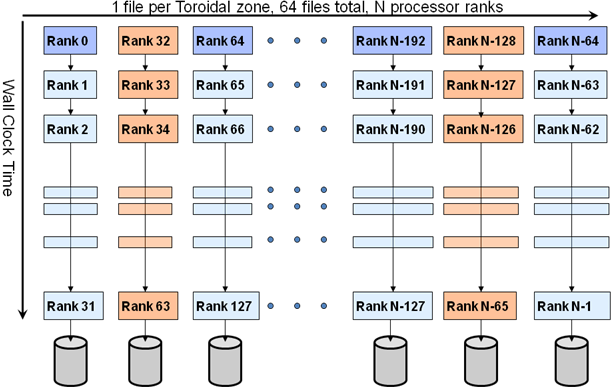
\includegraphics[width=290pt, height=185pt]{figures/mpi-method-serialized-opens.png}
\caption{Server-friendly metadata approach: offset the create/open in time}
\label{fig:serialized-open}
\end{center}
\end{figure}

We built the MPI transport method, mainly with Lustre in mind because it has been 
the primary parallel storage service we have available. However, other file-system-specific 
tunings are certainly possible and fully planned as part of this transport method 
system. For each new file system we encounter, a new transport method implementation 
tuned for that file system, and potentially that platform, can be developed without 
impacting any of the scientific code.

The MPI transport method is the most mature, fully featured, and well tested method 
in ADIOS. We recommend to anyone creating a new transport method that they study 
it as a model of full functionality and some of the advantages that can be made 
through careful management of the storage resources.

\subsection{MPI\_LUSTRE}

The MPI\_LUSTRE method is the MPI method with stripe alignment to achieve even 
greater write performance on the Lustre file system. Each writing process' data 
is aligned to Lustre stripes. This results in better parallelization of the storage 
elements. The drawback of using this method is that empty chunks are created between 
the data sets of the separate processes in the output file, and thus the file size 
is larger than with using the MPI method. The size of an empty space is the difference 
between the size of the output data of one writing process and the total size of 
Lustre stripes that can hold that amount of data, so that the next writing process' 
output starts aligned with another stripe. Choose the stripe size for the output 
file therefore carefully, to make the empty space as small as possible. 

The following XML snippet shows how to use the MPI\_LUSTRE method in ADIOS. 
\begin{lstlisting}[language=XML]
<method group="temperature" method="MPI_LUSTRE">
	stripe_count=16,stripe_size=4194304,block_size=4194304 
</method>
\end{lstlisting}

There are three key parameters used in this method.
\begin{itemize}
\item \textbf{stripe\_count} specifies how many storage targets to 
use for the whole output file. If not set, the default value is 4.

\item \textbf{stripe\_size}  specifies Lustre stripe size in bytes. 
If not set, the default value is 1048576 (i.e. 1 MB).

\item \textbf{block\_size}   specifies the size of each I/O write 
request. As an example, if total data size to be written from one process is 800 
MB at a time, and you want ADIOS to issue twenty I/O write requests issued from 
one process to Lustre during the writing, then the block\_size should be 40MB.
\end{itemize}

Note in 1.3 and later releases, with Lustreapi option enabled in configuration, 
MPI\_LUSTRE sets the parameters automatically and therefore parameters in XML are 
not required.  The method automatically calculates the data size from each processor 
and sets the proper striping parameters. 

\subsection{MPI\_AGGR}
\label{section-method-mpiamr}

The MPI\_AGGR method is designed to maximize write performance for large scale
applications (more than 10,000 cores) that write out data from a large subset of
processors. 
%such as adaptive mesh refinement (AMR) on the Lustre file system. 
%In AMR-like applications, 
%each processor outputs varying amount of data and some can output very small size 
%data. 
Based upon MPI\_LUSTRE method, MPI\_AGGR further improves the write speed by 

\begin{enumerate}
\item aggregating data from multiple MPI processors into large chunks. This effectively 
increases the size of each request and reduces the number of I/O requests.
\item threading the metadata operations such as file open. Users are encouraged to 
call adios\_open and adios\_group\_size API as early as possible. In case Lustre 
MDS has a performance hit, the overall metadata performance won't be affected. 
The following code snippet shows a typical way of using this method to improve 
metadata performance.
\begin{lstlisting}[language=XML]
adios_open(...); 
adios_group_size(...);
...... 
//do your computation
...... adios_write(..); 
adios_write(..); 
adios_close(..);
\end{lstlisting}

\item further removing communication and wide striping overhead by writing out subfiles. 
Please refer to POSIX method on how to read data from subfiles.
\end{enumerate}

The following XML snippet shows how to use MPI\_AGGR method in ADIOS.

There are two key parameters used in this method.

\begin{lstlisting}[language=XML]
<method group="tracers" method="MPI_AGGR"> 
	num_aggregators=24;num_ost=672
</method>
\end{lstlisting}

\begin{itemize}
\item \textbf{num\_aggregators} specifies the number of aggregators 
to use.
\item \textbf{num\_ost }specifies the number of Lustre storage targets 
 available in the file system. Note this parameter is mandatory if ``---with-lustre'' 
option is not given during ADIOS configuration.
\end{itemize}

For example, if you have an MPI job with 120,000 processors and the number of aggregator 
is set to 2400, then each aggregator will aggregate the data from 120,000/2400=50 
processors.

ADIOS MPI\_AGGR method allocates stand-alone internal buffers for aggregating data. 
As opposed to ADIOS buffer (the size of which is set from XML file), these buffers 
are allocated separately and the total size (on one processor) is twice the ADIOS 
group size. User needs to make sure each process has enough memory when using this 
method.  

Note that in 1.3 and later releases, with Lustreapi option enabled in configuration, 
MPI\_AGGR sets the parameters automatically and therefore parameters in XML are 
not required. The method automatically calculates the data size from each processor 
and sets the proper aggregation parameters. Also note that in previous versions
of ADIOS (before 1.4), the MPI\_AGGR method was refered to as the MPI\_AMR
method. 


\subsection{VAR\_MERGE}
\label{section-method-varmerge}
The VAR\_MREGE method is designed to extends the capability of current ADIOS
methods to address the I/O challenges for applications
that write out small variables at scale. During data output, 
VAR\_MERGE merges the small variable blocks from intensive chunking into
larger data chunks with their spatial localities are reserved. The benefits
are: 1) less contention at storage side during data
output; 2) frequent read and seek operations can be avoided during reading.
An example is given in Figure~\ref{fig:sar}. 


\begin{figure}[htbp]
\begin{center}
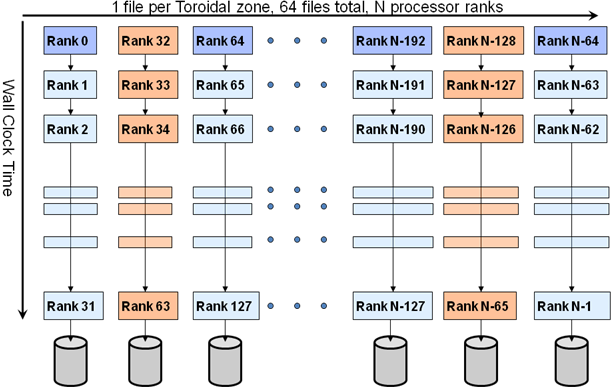
\includegraphics[width=290pt, height=185pt]{figures/mpi-method-serialized-opens.png}
\caption{Spatial Aggregation to merge small data blocks into large data
    chunks}
\label{fig:sar}
\end{center}
\end{figure}


The following XML snippet shows how to use VAR\_MERGE method in ADIOS.
There are two key parameters used in this method.

\begin{lstlisting}[language=XML]
<method group="test" method="VAR_MERGE"> chunk_size=2097152, io_method=MPI_AGGR, io_parameters=num_aggregators=24;num_ost=672
</method>
\end{lstlisting}

\begin{itemize}
\item \textbf{chunk\_size} specifies the chunk size after merging. If
merging current data chunk leads to a chunk size that is larger than this
value, merging will not be performed. The default value is 2MB without  
specification in XML.  

\item \textbf{io\_method} the underlying I/O method for data output.  
VAR\_MERGE can work with any existing ADIOS transport method. 

\item \textbf{io\_parameters} the parameters required for using the io\_method 
\end{itemize}

For example, if you want to merge data chunks into 4MB chunks and use
MPI\_LUSTRE method to write out data, your XML looks like:  

\begin{lstlisting}[language=XML]
<method group="test" method="VAR_MERGE"> chunk_size=4194304,
    io_method=MPI_LUSTRE, io_parameters=stripe_count=128,stripe_size=4194304
</method>
\end{lstlisting}

Here we specified the data to be placed on 128 storage targes, and the stripe
size is 4MB.
Note that current VAR\_MERGE method only supports 1D, 2D and 3D variables.
The maximum level of aggregation is 2 due to the consideration of
merging overhead.  

\subsection{Dataspaces}
\label{section-method-dataspaces}

Dataspaces is an asynchronous I/O transfer method within ADIOS that enables low-overhead, 
high-throughput data extraction from a running simulation. Dataspaces consists of two 
main components: (1) a client module using the ADIOS Dataspaces method, and (2)
a dataspaces\_server module. Internally, 
Dataspaces uses RDMA to implement the communication, coordination, and data transport 
between the clients and the dataspaces\_server modules.

The dataspaces clients use a light-weight library that provides the asynchronous
I/O API to be used by ADIOS. It is integrated with the ADIOS layer and the
functionality is exposed through the ADIOS write/read semantics. 
%It integrates with the ADIOS layer by extending the generic ADIOS data transport 
%hooks. 
The ADIOS layer is used to collect and encode the data written 
by the application into a local transport buffer. Once it has collected data from 
an application, the transport method notifies the dataspaces\_server through a coordination channel 
that it has data available to send out. At this point, the control is
transferred back to the application, while the data is asynchronously extracted 
by the dataspaces\_server.

The dataspaces\_server module is a stand-alone service that runs independently of a simulation 
on a set of dedicated nodes in the 
{\em staging area}. It transfers data from the application through RDMA,  
and can save it to local storage system, e.g., the Lustre file system, stream it to 
remote sites, e.g., auxilliary clusters, or serve it directly from the staging area to 
other applications. One instance of the dataspaces\_server can service multiple applications 
 in parallel. Further, the server can run in cooperative mode (i.e., multiple 
instances of the server cooperate to service the application in parallel and to balance 
load). The dataspaces\_server receives notification messages from the transport method, schedules 
the requests, and initiates the data transfers  in parallel. The 
server schedules and prioritizes the data transfers while the simulation is computing 
in order to overlap data transfers with computations, to maximize data throughput, 
and to minimize the overhead on the application.

Dataspaces is an asynchronous method available in ADIOS, that can be selected by specifying 
the transport method in the external ADIOS XML configuration file as ``Dataspaces''.

\begin{lstlisting}[language=XML, caption=Select Dataspaces as a transport method in the configuration file example.]
<method group="fluxdiag" method="Dataspaces"/>
\end{lstlisting}

To make use of the Dataspaces transport, an application job needs to also run the dataspaces\_server 
component together with the application. The server should be configured and started 
before the application as a separate job in the system. For example:

\begin{lstlisting}[language=bash, caption=Start the server component in a job file first.]
aprun -n $SPROC ./dataspaces_server -s $SPROC -c $PROC &> log.server &
\end{lstlisting}

The variable \$SPROC represents the number of server instances to run, and the 
variable \$PROC represents the number of application processes. For example if 
the job script runs a coupling scenario with two applications that run on 128 and 
432 processors respectively, then the value of \$PROC is 560. The `\&' character 
at the end of the line would place the `aprun' command in the background, and will 
allow the job script to continue and run the other applications. The server processes 
produce a configuration file, i.e., `conf' that is used by the application  
to connect to the servers. This file contains identifying information of the 
master server, which coordinates the client registration 
and discovery process. The job script should wait for the servers to start-up and 
produce the `conf' file before starting the client application processes. 
%, which it can then export to environment variables, e.g., 
%P2TNID, and P2TPID. 
Once ADIOS is initialized in the application, this configuration file is parsed
to provide the rendevouz information. 

\begin{lstlisting}[language=C, caption=Wait for server start-up completion and export the configuration to environment variables.]
while [ ! -f conf ]; do
	echo "Waiting for servers to start-up"
	sleep 2s
done


while read line; do
	export set "${line}"
done < conf
\end{lstlisting}

The server component will terminate automatically when the applications finish. 
The clients  will send an unregister message to the server before 
they finish execution, and the servers will exit after they receive \$PROC unregister 
messages.

%% The Dataspaces transport method is experimental and is not included with the public version 
%% of the ADIOS source code in this release; however it is available for use on the 
%% XT4 and XT5 machines at ORNL.

\subsection{DIMES}
\label{section-method-dimes}
% DIstributed MEmory Space (DIMES)
DIMES is another asynchronous I/O transfer method within ADIOS that enables low-
latency, scalable data extraction from a running simulation. It is designed to enable M$
\times$N parallel data redistribution between tightly coupled applications, which 
essentially performs RDMA-based memory-to-memory transfers of distributed data such 
as global arrays from M processes of one application to N processes of another application.

Both DIMES and Dataspaces methods are implemented based upon the open source 
software library DataSpaces. However, unlike Dataspaces method which implements 
memory-to-memory data sharing using dedicated server nodes in the \emph{staging 
area}, DIMES method implements the parallel data redistribution through point-to-point 
transfers directly between processes of data writing and reading applications, and thus 
bypass the \emph{staging area}. 

For applications using the ADIOS DIMES method, the new functionality is exposed 
through the ADIOS write/read semantics. ADIOS layer is used to collect data written by 
the application into a local RDMA memory buffer as data objects that can 
be remotely accessed through the underlying RDMA get operations. Once data is 
successfully copied from the application space, the control is transferred back to the 
application, then the simulation data can be asynchronously extracted and redistributed 
to the coupled reading applications. 

Though the DIMES methods does not need simulation data to be transferred to the 
\emph{staging area}, a stand-alone server module is still required for constructing a 
distributed directory service to keep track of the in-memory data objects. Internally, client 
applications would query the service to locate required data objects, and then perform 
the subsequent RDMA-based parallel data transfers. 

DIMES method can be selected by specifying the transport method in the external 
ADIOS XML configuration file (as below).

\begin{lstlisting}[language=XML, caption=Select DIMES as a transport method in the configuration file example.]
<method group="fluxdiag" method="DIMES"/>
\end{lstlisting}

The dataspaces\_server component is extended to support the data locating service 
mentioned above. To make use of the DIMES method, a job needs to also run the 
dataspaces\_server with the applications. Each dataspaces\_server instance 
needs to run on one dedicated processor core, and multiple sever instances can be 
started in parallel to support the data locating service for larger scale applications. 
Instructions on how to configure and run the dataspaces\_server can be found in 
section~\ref{section-method-dataspaces}.


\subsection{Flexpath}
\label{section-method-flexpath}
Flexpath is an asynchronous data transport method built to ensure scalable I/O through the use of staging areas. It is built on top of the EVPath event-driven messaging library \url{http://www.cc.gatech.edu/systems/projects/EVPath/}, which allows for the creation of arbitrary network overlays. Data sent through EVPath is serialized with the Fast, Flexible Serialization (FFS) library, and also allows for additional metadata to be appended to the datastream through the use of separately addressable attributes. To provide high-performance, Flexpath takes advantage of EVPath features such as {\em multiqueue stones} and {\em C-on-Demand (COD)} dynamic code generation.

Flexpath also works on top of several popular high-end network interfaces, such as Infiniband, Portals, and Gemini. See the intallation section for information on how to use this functionality. 


\subsection{PHDF5}

HDF5, as a hierarchical File structure, has been widely adopted for data storage 
in various scientific research fields.  Parallel HDF5 (PHDF5) provides a series 
of APIs to perform the I/O operations in parallel from multiple processors, which 
dramatically improves the I/O performance of the sequential approach to read/write 
an HDF5 file. In order to make the difference in transport methods and file formats 
transparent to the end users, we provide a mechanism that write/read an HDF5 file 
with the same schema by keeping the same common adios routines with only one entry 
change in the XML file. This method provides users with the capability to write 
out exactly the same HDF5 files as those generated by their original PHDF5 routines. 
Doing so allows for the same analysis tool chain to analyze the data. 

Currently, HDF5 supports two I/O modes: independent and Collective read or write, 
which can use either the MPI or the POSIX driver by specifying the dataset transfer 
property list in H5Dwrite function calls. In this release, only the MPI driver 
is supported in ADIOS.
This requires that every process participates in the writing of each variable. 

Note: Do not expect better performance with ADIOS/PHDF5 than with PHDF5 itself. ADIOS does not write differently to a HDF5 formatted file, it simply uses PHDF5 function calls to write out data. 

%later on, both I/O drivers will be supported by changing 
%the attribute information for PHDF5 method elements in XML. 

\subsection{NetCDF4}

Another widely accepted standard file format is NetCDF, which is the most frequently 
used file format in the climate and weather research communities.  Beginning with 
the NetCDF 4.0 release, NetCDF has added PHDF5 as a new option for data storage 
called the ``netcdf-4 format''.  When a NetCDF4 file is opened in this new format, 
NetCDF4 inherits PHDF5's parallel I/O capabilities.

The NetCDF4 method creates a single shared filed in the ``netcdf-4 format'' and 
uses the parallel I/O features.  The NetCDF4 method supports multiple open files. 
 To select the NetCDF4 method use ``NC4'' as the method name in the XML file.

\textbf{Restrictions:} Due to the collective nature of the NetCDF4 API, there are 
some legal XML files that will not work with the NetCDF4 method.  The most notable 
incompatibility is an XML fragment that creates an array variable without a surrounding 
global-bounds.  Within the application, a call to adios\_set\_path() is used to 
add a unique prefix to the variable name.  A rank-based prefix is an example. 

\begin{lstlisting}[language=XML, caption=Example XML]
<?xml version="1.0"?> 
<adios-config host-language="C">
	<adios-group name="atoms " coordination-communicator="comm"> 
		<var name="nparam" type="integer"/>
		<var name="ntracked" type="integer"/>
		<var name="atoms " type="real" dimensions="nparam,ntracked"/> 
	</adios-group>
	<method group="atoms" method="NC4"/> 
	<buffer size-MB="1" allocate-time="now"/> 
</adios-config>
\end{lstlisting}

\begin{lstlisting}[language=C, caption=Example C source]
char path[1024];
adios_init ("config.xml", comm);
adios_open (&adios_handle, "atoms", filename, "w", comm); 
sprintf(path, "node_%d_", myrank); 
adios_set_path(adios_handle, path);
#include "gwrite_atoms.ch" 
adios_close (adios_handle); 
adios_finalize (myrank);
\end{lstlisting}

This technique is an optimization that allows each rank to creates a variable of 
the exact dimensions of the data being written.  In this example, each rank may 
be tracking a different number of atoms.

The NetCDF4 collective API expects each rank to write the same variable with the 
same dimensions.  The example violates both of these expectations.

Note: NetCDF4 files created in the new ``netcdf-4 format'' cannot be opened with 
existing tools linked with NetCDF 3.x.  However, NetCDF4 provides a backward compatibility 
API, so that these tools can be relinked with NetCDF4.  After relink, these tools 
can open files in the ``netcdf-4 format''.


\section{Research Methods}

ADIOS provides an easy plug-in mechanism for users or developers to design their 
own transport method. A step-by-step instruction for inserting a new I/O method 
is given in the Developer's manual. Users are likely to choose the best method from among 
the supported or customized methods for the running their platforms, thus avoiding 
the need to verify their source codes due to the switching of I/O methods.

%% \section{Asynchronous methods}

\subsection{Network Scalable Service Interface (NSSI)}

The Network Scalable Service Interface (NSSI) is a client-server development framework 
for large-scale HPC systems.  NSSI was originally developed out of necessity for 
the Lightweight File Systems (LWFS) project, a joint effort between researchers 
at Sandia National Laboratories and the University of New Mexico.  The LWFS approach 
was to provide a core set of fundamental capabilities for security, data-movement, 
and storage, and allow extensibility through the development of additional services. 
 The NSSI framework was designed to be the vehicle to enable the rapid development 
of such services.

The NSSI method is composed of two components - a client method and a staging service. 
 The client method does not perform any file I/O.  Instead, all ADIOS operations 
become requests to the staging service.  The staging service is an ADIOS application, 
which allows the user to select any ADIOS method for output.  Client requests fall 
into two categories - pass-through and cached.  Pass-through requests are requests 
that are synchronous on the staging service and return an error immediately on 
failure.  adios\_open() is an example of a pass-through request.  Cached requests 
are requests that are asynchronous on the staging service and return an error at 
a later time on failure.  adios\_write() is an example of a cached request.  All 
data cached for a particular file is aggregated and flushed when the client calls 
adios\_close().

Each component requires its own XML config file.  The client method can be selected 
in the client XML config using ``NSSI'' as the method.  The service XML config 
must be the same as the client XML config except that the method is ``NSSI\_FILTER''. 
 When the NSSI\_FILTER method is selected, the ``submethod'' parameter is required. 
 The ``submethod'' parameter specifies the ADIOS method that the staging service 
will use for output.  Converting an existing XML config file for use with NSSI 
is illustrated in the following three Figures.

\begin{lstlisting}[language=XML, caption=Example Original Client XML]
<method method="MPI" group="atoms">max_storage_targets=160</method>
\end{lstlisting}

\begin{lstlisting}[language=XML, caption=Example NSSI Client XML]
<method method="NSSI" group="atoms"/>
\end{lstlisting}

\begin{lstlisting}[language=XML, caption=Example NSSI Staging Service XML]
<method method="NSSI_FILTER" group="atoms"> 
	submethod="MPI" ;subparameters="max_storage_targets=160"
</method>
\end{lstlisting}

After creating new config files, the application's PBS script (or other runtime 
script) must be modified to start the staging service prior to application launch 
and stop the staging service after application termination. The ADIOS distribution 
includes three scripts to help with these tasks.

The start.nssi.staging.sh script launches the staging service.  start.nssi.staging.sh 
takes two arguments - the number of staging services and an XML config file.

The create.nssi.config.sh script creates an XML file that the NSSI method uses 
to locate the staging services.  create.nssi.config.sh takes two arguments - the 
name of the output config file and the name of the file containing a list of service 
contact info.  The service contact file is created by the staging service at startup. 
 The staging service uses the ADIOS\_NSSI\_CONTACT\_INFO environment variable to 
determine the pathname of the contact file.

The kill.nssi.staging.sh script sends a kill request to the staging service.  kill.nssi.staging.sh 
 takes one argument - the name of the file containing a list of service contact 
info (ADIOS\_NSSI\_CONTACT\_INFO).  The staging service will gracefully terminate.

\begin{lstlisting}[language=bash, caption={Example PBS script with NSSI Staging Service}, label=list-nssi-pbs-script]
#!/bin/bash
#PBS -l walltime=01:00:00,size=128

export RUNTIME_PATH=/tmp/work/$USER/genarray3d.$PBS_JOBID
mkdir -p $RUNTIME_PATH
cd $RUNTIME_PATH


export ADIOS_NSSI_CONTACT_INFO=$RUNTIME_PATH/nssi_contact.xml
export ADIOS_NSSI_CONFIG_FILE=$RUNTIME_PATH/nssi_config.xml 
$ADIOS_DIR/scripts/start.nssi.staging.sh 4 \
	$RUNTIME_PATH/genarray3d.server.xml >server.log 2>&1 &
sleep 3
$ADIOS_DIR/scripts/create.nssi.config.sh \
	$ADIOS_NSSI_CONFIG_FILE $ADIOS_NSSI_CONTACT_INFO 

aprun -n 64 $ADIOS_SRC_PATH/tests/genarray/genarray \
	$RUNTIME_PATH/test.output 4 4 4 128 128 80 >runlog 

$ADIOS_DIR/scripts/kill.nssi.staging.sh $ADIOS_NSSI_CONTACT_INFO
\end{lstlisting}

Listing~\ref{list-nssi-pbs-script} is a example PBS script that highlights the changes required to launch 
the NSSI staging service.

\textbf{Required Environment Variables.}  The NSSI Staging Service requires that 
the ADIOS\_NSSI\_CONTACT\_INFO variable be set.  This variable specifies the full 
pathname of the file that the service uses to save its contact information.  Depending 
on the platform, the contact information is a NID/PID pair or a hostname/port pair. 
 Rank0 is responsible for gathering the contact information from all members of 
the job and writing the contact file.  The NSSI method requires that the ADIOS\_NSSI\_CONFIG\_FILE 
variable be set.  This variable specifies the full pathname of the file that contains 
the complete configuration information for the NSSI method.  A configuration file 
with contact information and reasonable defaults for everything else can be created 
with the create.nssi.config.sh script.

\textbf{Calculating the Number of Staging Services Required.}  Remember that all 
adios\_write() operations are cached requests.  This implies that the staging service 
must have enough RAM available to cache all data written by its clients between 
adios\_open() and adios\_close().  The current aggregation algorithm requires a 
buffer equal to the size of the data into which the data is aggregated.  The start.nssi.staging.sh 
script launches a single service per node, so the largest amount of data that can 
be cached per service is 50\% of the memory on a node minus system overhead.  System 
overhead can be estimated at 500MB.  If a node has 16GB of memory, the amount of 
data that can be cached is 7.75GB ((16GB-500MB)/2).  To balance the load on the 
staging services, the number of clients should be evenly divisible by the number 
of staging services.

\textbf{Calculating the Number of Additional Cores Required for Staging.}  The 
NSSI staging services run on compute nodes, so additional resources are required 
to run the job.  For each staging service required, add the number of cores per 
node to the size of the job.  If each node has 12 cores and the job requires 16 
staging services, add 192 cores to the job.

The NSSI transport method is experimental and is not included with the public version 
of the ADIOS source code in this release; however it is available for use on the 
XT4 and XT5 machines at ORNL.

\subsection{DataTap}

DataTap is an asynchronous data transport method built to ensure very high levels 
of scalability through server-directed I/O. It is implemented as a request-read 
service designed to bridge the order-of-magnitude difference between available 
memories on the I/O partition compared with the compute partition. We assume the 
existence of a large number of compute nodes producing data (we refer to them as 
``\textit{DataTap }clients'') and a smaller number of I/O nodes receiving the data 
(we refer to them as ``\textit{DataTap }servers'') (see Figure~\ref{fig:datatap-arch}). 

\begin{figure}[htbp]
\begin{center}
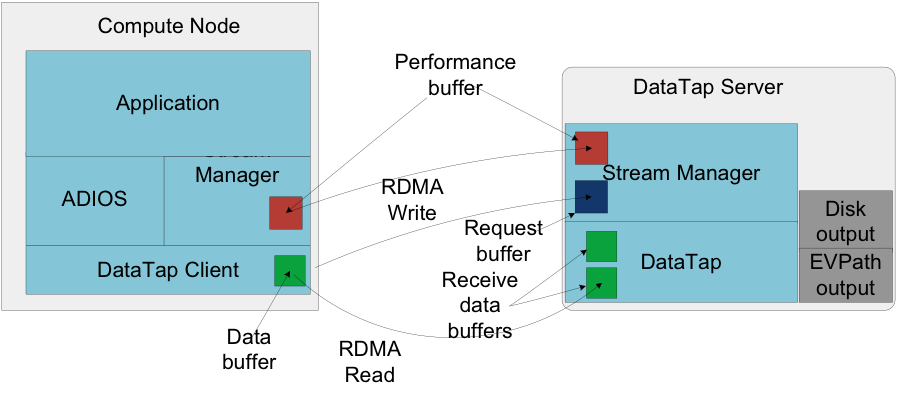
\includegraphics[width=222pt, height=97pt]{figures/datatap-architecture.png}
\caption{DataTap architecture}
\label{fig:datatap-arch}
\end{center}
\end{figure}


Upon application request, the compute node marks up the data in PBIO format and 
issues a request for a data transfer to the server. The server queues the request 
until sufficient receive buffer space is available. The major cost associated with 
setting up the transfer is the cost of allocating the data buffer and copying the 
data. However, this overhead is small enough to have little impact on the overall 
application runtime. When the server has sufficient buffer space, a remote direct 
memory access (RDMA) read request is issued to the client to read the remote data 
into a local buffer. The data are then written out to disk or transmitted over 
the network as input for further processing in the I/O Graph. 

We used the Gyrokinetic Turbulence Code (GTC) as an experimental tested for the 
DataTap transport. GTC is a particle-in-cell code for simulating fusion within 
tokamaks, and it is able to scale to multiple thousands of processors. In its default 
I/O pattern, the dominant I/O cost is from each processor writing out the local 
particle array into a file. Asynchronous I/O reduces this cost to just a local 
memory copy, thereby reducing the overhead of I/O in the application.

The DataTap transport method is experimental and is not included with the public 
version of the ADIOS source code in this release; however it is available for use 
on the XT4 and XT5 machines at ORNL.


%\section{Other research methods at ORNL}

\subsection{MPI-CIO}

MPI-IO defines a set of portable programming interfaces that enable multiple processes 
to have concurrent access to shared files [1]. It is often used to store and retrieve 
structured data in their canonical order. The interfaces are split into two types: 
collective I/O and independent I/O. Collective functions require all processes 
to participate. Independent I/O, in contrast, requires no process synchronization.

Collective I/O enables process collaboration to rearrange I/O requests for better 
performance [2,3]. The collective I/O method in ADIOS first defines MPI fileviews 
for all processes based on the data partitioning information provided in the XML 
configuration file. ADIOS also generates MPI-IO hints, such as data sieving and 
I/O aggregators, based on the access pattern and underlying file system configuration. 
The hints are supplied to the MPI-IO library for further performance enhancement. 
The syntax to describe the data-partitioning pattern in the XML file uses the \texttt{<}global-bounds 
dimensions offsets\texttt{>} tag, which defines the global array size and the offsets 
of local subarrays in the global space. 

The global-bounds element contains one or more nested var elements, each specifying 
a local array that exists within the described dimensions and offset.  Multiple 
global-bounds elements are permitted, and strictly local arrays can be specified 
outside the context of the global-bounds element.

As with other data elements, each of the attributes of the global-bounds element 
is provided by the adios\_write call. The dimensions attribute is specified by 
all participating processes and defines how big the total global space is.  This 
value must agree for all nodes. The offset attribute specifies the offset into 
this global space to which the local values are addressed. The actual size of the 
local element is specified in the nested var element(s).  For example, if the global 
bounds dimension were 50 and the offset were 10, then the var(s) nested within 
the global-bounds would all be declared in a global array of 50 elements with each 
local array starting at an offset of 10 from the start of the array.  If more than 
one var is nested within the global-bounds, they share the declaration of the bounds 
but are treated individually and independently for data storage purposes. 

This research method is installed on Jaguar at ORNL only but is not part of the 
public release.

\subsection{MPI-AIO}

The initial implementation of the asynchronous MPI-IO method (MPI-AIO) is patterned 
after the MPI-IO method. Scheduled metadata commands are performed with the same 
serialization of MPI\_Open calls as given in Figure~\ref{fig:serialized-open}.

The degree of I/O synchronicity depends on several factors. First, the ADIOS library 
must be built with versions of MPI that are built with asynchronous I/O support 
through the MPI\_File\_iwrite, MPI\_File\_iread, and MPI\_Wait calls. If asynchronous 
I/O is not available, the calls revert to synchronous (read blocking) behavior 
identical to the MPI-IO method described in the previous section. 

Another important factor is the amount of available ADIOS buffer space. In the 
MPI-IO method, data are transported and ADIOS buffer allocation is reclaimed for 
subsequent use with calls to adios\_close (). In the MPI-AIO method, the ``close'' 
process can be deferred until buffer allocation is needed for new data. However, 
if the buffer allocation is exceeded, the data must be synchronously transported 
before the application can proceed.

The deferral of data transport is key to effectively scheduling asynchronous I/O 
with a computation. In ADIOS version 1.4, the application explicitly signals that 
data transport must be complete with intelligent placement of the adios\_close 
() call to indicate when I/O must be complete. Later versions of ADIOS will perform 
I/O between adios\_begin\_calculation and adios\_end\_calculation calls, and complete 
I/O on adios\_end\_iteration calls.

This research module is not released in ADIOS 1.4.


\chapter{Data Transformations}
\label{sec:transform_plugins}
The ADIOS data transformations framework, new in version 1.6, enables on-the-fly, transparent ``data transformations'' during the ADIOS
write phase. Data transformations are a class of algorithms that change the format of a variable's data for some purpose
(for example, compression to reduce storage footprint).
Data transforms in ADIOS are fully configurable on a per-variable basis; for instance, one variable
may be compressed while another has no transform applied.

While ADIOS comes with lossless compression transform plugins, it is possible for plugin developers to implement new plugins.
Possibilities include: lossy compression, layout optimization for increased spatial locality,
on-the-fly value indexing, and precision-based and sampling-based level-of-detail encodings.

It is important to note that data transforms are \emph{runtime configurable}, meaning selecting a new configuration of data
transforms for variables in the ADIOS XML does \emph{not} require recompiling the application (analogously to I/O transport
selection via the XML). Furthermore, beyond editing the XML, no other changes are required to application code to use data
transforms during writing or reading. This makes it possible to easily experiment with the effects of a variety of compression
methods and parameters in an application.

\section{Writing with data transformations}
Data transforms are selected via the ADIOS XML file, as follows:

\begin{lstlisting}[language=XML]
<var name="/temperature"
     dimensions="..."
     type="adios_real"
     transform="zlib"    <!-- Add this attribute -->
  />
\end{lstlisting}

The above snippet of XML will cause the variable "/temperature" to be compressed using zlib, assuming ADIOS was configured with zlib support
(see Section~\ref{sec:installation-data-transforms} for configuration instructions). ADIOS 1.6 includes support for transform plugins
``zlib,'' ``bzip2,'' and ``szip'' (see Table~\ref{tbl:data-transforms-summary}).
Some transform plugins accept parameters, which are appended after a colon following the transform name.
For instance, zlib accepts an optional compression level between 1 and 9, with 1 being the fastest and
9 being the highest compression ratio. Setting the level to 5 would be accomplished as follows:

\begin{lstlisting}[language=XML]
<var name="/temperature"
     ...
     transform="zlib:5"/>
\end{lstlisting}

In fact, all three lossless compression plugins (zlib, bzip2, and szip) currently accept this same
1-to-9 compression level. The default compression for each library is used if this parameter is
omitted, which is typically the case.

\begin{table}%
\begin{tabular}{l|l|l}
\textbf{Transform name in XML} & \textbf{Description} & \textbf{Other info} \\
\hline
zlib & zlib lossless compression & requires the zlib external library \\
\hline
bzip2 & bzip2 lossless compression & requires the bzip2 external library \\
\hline
szip & szip lossless compression & requires the szip external library \\
\end{tabular}
\caption{Summary of data transform plugins included in ADIOS}
\label{tbl:data-transforms-summary}
\end{table}

Data transformations that have been selected for a variable are applied at write time, during the call to \verb+adios_write()+.
Data transforms are applied on a per-core basis, so no additional data movement or other communication is incurred.
The resultant re-formatted data is then written using whatever I/O transport method is active.

\section{Reading with data transformations}
On the read side, no changes to application code are necessary. If a variable being read was transformed when written
(e.g., zlib compressed), the transformation will be inverted automatically, returning the original data,
with no changes needed to reader application.

\section{Considerations when selecting data transforms}
When deciding whether to apply data transforms, and which transform methods to use, depends on a few factors.
Since the built-in data transforms in ADIOS are compression routines, we will focus on this case, but much of
this discussion applies generally to any data transform.

First, because the transform is applied at write time, the user must consider the tradeoff between the CPU cost of applying
the transform (e.g., compression time) with the expected benefits (reduced storage space, and potentially reduced I/O time).
The balance point for a particular application can only be determined through experimentation, but for compression,
the more compressible the user's data is, the beneficial a compression transform may be.

Second, note that some transforms, including compression, necessarily make some read operations more costly. This is because
chunks of variable data in the file (the piece of the variable in each process group, to be precise) will be compressed
in its entirety, and so during reads, any process group chunk that is touched must be read and decompressed fully, whereas
without compression, some of the chunk might have been omitted from the read.

As before, experimentation is the only way to definitively identify application- and read-pattern-specific read overhead.
However, as a rule, smaller PG sizes and read access
patterns that access large parts of PGs (e.g., full timestep reads and subvolume selections, as opposed to plane cuts and
point selections) experience less overhead. For example, very large PG sizes (>10MB per variable per writing process per timestep)
combined with read patterns that touch small pieces of many PGs (such as plane cuts) can experience substantial overhead.
In contrast, checkpoint-restart-like access patterns that are highly aligned to PG boundaries,
this overhead should be negligible, and overall performance improvement is possible via reduced I/O time given a high enough compression
ratio.

Finally, note the compatibility limitations described in the next section.

\section{Compatibility}
As mentioned above, data transforms work seamlessly with existing read and write APIs; only the addition of the "transform" attribute
in the XML is required to invoke a data transform.

As for I/O transports, in this release only file-based transports are supported while data transforms are active.
This includes the \verb+POSIX+, \verb+MPI+, \verb+MPI_LUSTRE+, and \verb+MPI_AGGREGATE+ write transports and
the \verb+READ_BP+ read transport. Additionally,
when reading transformed data, only the file access mode is currently supported (i.e., streaming mode is unsupported).
Of course, none of these limitations apply to use of ADIOS when no data transforms is active
(i.e., no "transform" attributes in the XML for writes and no transformed variables are accessed for reads).

As a final note, due to the way in which space allocation occurs under compression data transforms,
applying compression in combination with certain I/O transports (including
\verb+MPI+ and \verb+MPI_LUSTRE+) will produce ``sparse files'' with ``holes'' (unused space).
While this may avoided entirely by using other transports (including \verb+MPI_AGGREGATE+ and
\verb+POSIX+) sparse files are not necessarily bad. Sparse files do not consume extra disk space or
I/O time on most filesystems (including Lustre, GPFS, PVFS and modern ext Linux filesystems),
and standard Linux file manipulation tools (including cp and rsync) usually handle such files efficiently.
Only if moved/copied using a tool (besides cp or rsync) that ``materializes'' them into normal ``dense files''
will they begin consume more space. A file can be tested for sparsenesss by comparing the output of ``du -h <file>'' and
``ls -l <file>'' (the former reports actual disk space used, whereas the latter reports logical file size;
for sparse files, these quantities differ significantly).
Again, sparse files may be completely avoided by using \verb+MPI_AGGREGATE+ or \verb+POSIX+.

As this is the first release of the ADIOS data transformation framework, optimization and improvements are ongoing, and
in the future many of these restrictions are likely to be ameliorated.


\chapter{ADIOS Read API}
\label{chapter:read_api}

\section{Introduction}

The second version of the ADIOS Read API (introduced in ADIOS 1.4) is designed to handle both files on disk and data sets in memory staging areas. Non-blocking and chunking read is introduced to enable concurrent processing of some part of the requested data while other parts are being retrieved for methods that support it.  A Selection interface is introduced to define subsets of datasets other than a simple bounding box. 


\subsection{Changes from version 1}
The original version of ADIOS Read API (in ADIOS releases 1.0--1.3.1) provides a (1) grouped view of variables in an ADIOS-BP file with (2) time as an extra dimension. ADIOS applications can write multiple, separate groups of variables into one file. They can also write multiple steps of a group into one file. When opening a file for reading, each group is conceptually separated and thus has to be opened separately. Also, an N--dimensional variable with multiple steps is presented as an N+1--dimensional variable, with time represented as the slowest dimension (like in NetCDF). These two representations have been eliminated in the new API, both for the sake of supporting streams with the same API as files and thus enable the transition from file-based analytics and visualization to staging environments where data sets are passed around without touching permanent storage.

In the new API, all variables of all groups are presented at once when opening the file. Nevertheless, some extra functions are provided in the API to get the list of groups written into the file (\verb+adios_get_grouplist()+) and to restrict the view of variables and attributes to a certain group (\verb+adios_group_view()+) in case some application would need this artificial separation. 

Time is completely eliminated as a concept from the read API. Now one sees the output steps as they are; just steps. An N--dimensional variable written M times into the same file is represented as an N--dimensional variable with M steps available to read. From permanently stored datasets (files), the user can still read multiple steps at once and store in the user-provided contigous memory but with arguments separate from the spatial dimension specification.

\subsection{Concepts}

\begin{itemize}
    \item {\em Reader} is an application reading data using ADIOS
    \item {\em Writer} is an application writing output data using ADIOS
    \item {\em Reading methods} are different reading codes in ADIOS from which a Reader can choose one, e.g. for reading from a file, or from the memory of the Writer. 
\end{itemize}


\subsubsection{Staging}
Staging here means that data is in memory somewhere and an ADIOS method presents that data to a reader as a stream. That is, it has to be opened, its content can be discovered, it contains variables and attributes, and it has to be closed afterwards. Different staging scenarios exist and are under development by various teams:

\begin{itemize}
    \item A staging server with its own compute nodes and memory, stores the output of writing applications, allows connections from several applications and serves read requests. 
    \item A staging library embedded in the reading application, connects directly to a writing application and pulls the requested data out of the writer's memory. 
    \item A staging library like the above with the specialization that both writer and reader occupies the same (multi-core) compute node and shares memory.   
\end{itemize}

\noindent ADIOS 1.4 comes with the DataSpaces method that is an implementation of the first scenario. Methods for the other two scenarios are coming in the near future. 

\subsubsection{Streams and Steps}
Simulations usually write the same data set regularly over time, so a file or a series of files contains the same set of variables written many times. The dataset written between one adios\_open and adios\_close calls is called {\em STEP} and not "time" or "timesteps" to avoid confusing users about what time actually means. A {\em STREAM} differs from a file containing multiple steps only in the handling of steps. In a file on disk, all steps are available at all times to a reader. In a stream, only one step is available at a time to read, and as newer steps are becoming available from the writer, older steps may disappear. The ADIOS Read API provides two different open functions for streams and files. Nevertheless, a file can be handled in an application as a stream, i.e., by reading one step at a time, processing it, then advancing to the next step. Users are encouraged to write their code with streaming in mind, so that their file processing code can be used in a staging environment without code modification. 

\vspace{6pt}
\noindent {\bf Note:} A stream in ADIOS is {\bf not} a byte stream! The unit of the stream is one output Step of the Writer, so it still can be much larger than the available memory in the Reader.
\vspace{6pt}

In case of opening a file in file mode, each variable may have a different numberof steps, which is known at the time of opening the file. The number of steps value can be inquired for each variable separately (this value is always 1 for all variables in a stream). Then the application can read some steps of a variable at once, which may be different from the "global steps" written into the file. E.g., if a variable is written at every other output steps (1,3,5,...,n), then it will have half as many steps as the file itself has but its steps are addressed as 0,1,2...$\lceil n/2\rceil-1$.

In case of streams a step is the feature of the stream, not of the individual variables. There is no individual counting of the variables so the application has to count them itself if needed. 


\subsubsection{Locking strategies}
Locking is not used for files, but in a staging environment there are different strategies to deal with disappearing steps of datasets. A daredevil reader may tell the API to not block the writing application at all ({\em ADIOS\_LOCKMODE\_NONE}), i.e., to allow for loosing the opened data set any time if space is needed for storing newer steps of the writer's output. A safer way to handle complete steps is to lock the currently opened step ({\em ADIOS\_LOCKMODE\_CURRENT}). If the writer has more output in the meantime and there is not enough space for staging, an earlier or even a more recent step can be removed by the staging method. To ensure correct execution of  rigid readers, current and all more recent steps should be locked so that they can be read one-by-one without loosing them ({\em ADIOS\_LOCKMODE\_ALL}). This strategy, however, can certainly block the writing application if it has to wait for some available space to become free in the staging area.

Note, however, that specific staging methods may not support all locking mechanisms, or the actual locking mechanism would depend on their configuration and runtime set-up. E.g., the DataSpaces method in \adiosversion only supports the {\em ADIOS\_LOCKMODE\_CURRENT} locking strategy, although the DataSpaces server can also be started up with a custom locking that enforces synchronized steps of alternating writes and reads. The three locking options are kept in the read API with the hope that some staging methods would support all of them in the future. 

\subsubsection{Chunks}
Chunking allows for processing large data in small pieces concurrently while other pieces are being transferred.

\emph{Note: In \adiosversion, chunking is implemented only "functionally" in any method; all of them will just read the whole variable at once.}

A read request of a variable for one step can be served in multiple pieces. The reader should be able to receive parts of the whole requested dataset and process them one by one, instead of expecting the whole data set arriving in one piece, ordered in memory. We call these pieces or parts returned by the reading method to the reader as \emph{chunks}. In ADIOS, chunks are closely related to the individual outputs of writing processes. Therefore, readers should expect to receive one chunk per writer whose output partly matches the query.

\subsection{Selections}
Selection is some subset of a variable. ADIOS reading methods support 

\begin{itemize}
    \item Contiguous {\em Bounding Box}es (compact ranges in all dimensions of a variable), 
     \item A set of individual {\em Points}
    \item Individual selection of a block written by one writer process
         \item "Auto" selection for a special case of asking for locally available data in in-situ staging frameworks
\end{itemize}

\noindent Note that the bounding box was supported in the ADIOS Read API v1 implicitly, as extra arguments in the adios\_read\_var calls, and individual blocks were accessible with the special function adios\_read\_local\_var. 

All reading methods understand and can serve read requests over such selections.  

\section{How to use the read functions}
First, before opening a file/stream, we have to choose a reading method and initialize it with the \linebreak \verb+adios_read_init_method()+. Also, an \verb+adios_read_finalize_method()+ is necessary at the end of the application run. Note, that there is a separate initialization call for each read method the application intends to use.

A file has to be opened with \verb+adios_read_open_file(fname, method, comm)+ if the application wants to handle it as file (all steps accessible at once). A name, a read method and an MPI communicator should be provided. A stream (or a file handled as a stream) has to be opened with \linebreak
\verb+adios_read_open(fname, method, comm, lock_mode, timeout_sec)+.  A locking strategy has to be specified and some timeout can be specified for waiting for the stream to appear.  

In C, a transparent data struct is returned (\verb+ADIOS_FILE+), which enumerates the list of variables and attributes,  the current step and the available steps in the staging memory at the time of opening. The available steps are updated whenever seeking with \verb+adios_advance_step()+. Seeking is allowed to the next available step or to the last (newest) available step, with the possible errors of not finding any new step or finding that the stream has terminated. The current step can be released without advancing the step too, to free resources in the staging area. This optimization call is highly encouraged in every application to give free space to the writing application as early as possible. 

To read a subset of a variable, a selection object has to be created. The selection is independent from the variable (e.g. a bounding box) and from the opened file/stream, so it can be reused for reading many similar variables. 

When reading data, several read operations are first scheduled (\verb+adios_schedule_read_var()+), then \verb+adios_perform_reads()+ is called to start/do the actual reading. In blocking mode, this function returns when all reading has been finished and all result is stored in the user provided memory (provided separately for each variable in the schedule step). 

In non-blocking mode, this function returns as soon as possible and the application has to check for variables becoming available with \verb+adios_check_reads()+. This function returns zero or one "chunk".
If memory was provided to a variable in the schedule call, a single chunk will eventually be returned here that describes the whole variable. If memory was not provided, the chunking read mode should use an internal buffer in ADIOS to store and return a partial result. It depends on the size of the internal buffer and the number of writers of the requested piece that how many chunks will be needed for each scheduled read. Each chunk is a contiguous subset of the requested variable, but it is the application's own business how to reorganize the chunks into the complete request. This function returns one chunk at a time, which should be processed before calling this function again. It should be called repeatedly until the function tells the application that all reads have been completed.

Reading is concluded with closing the file/stream with \verb+adios_close()+ and deleting the ADIOS objects created to schedule the reading (selections with \verb+adios_selection_delete()+ and inquired structures with \verb+adios_free_varinfo()+).

\section{Notes}

\emph{Dimensions of arrays are reported differently for C and Fortran}.
When reading from a different language than writing (Fortran vs. C), 
the storage order of the dimensions 
is the opposite. Instead of transposing multidimensional arrays in memory to order 
the data correctly at read time, simply the dimensions are reported reversed. 

\emph{Metadata rich footer enables fast information retrieval}.
Since the BP file format is metadata rich, and the metadata is immediately accessible 
in the footer of the file, we can get a lot of information without accessing the file again
after the open call. 
The open function returns the list of variables and attributes. 
Type and dimensionality as well as the actual value of a scalar variable is returned by adios\_inq\_var.
Another inquiry extends the information with statistics (minimum, maximum, average and
standard deviation globally and for each writer process separately). Similarly, another inquiry
extends the information with dimensionality for each writer process 
(i.e. the detailed decomposition of a variable).


\emph{Steps start from 0}, even in Fortran applications (just because ADIOS is written in C, where everything starts from 0). 


\section{Read C API description}

Please consult the \verb+adios_read_v2.h+ for the data structures and functions discussed here. In the source code, do not include this header file directly, but \verb+adios_read.h+. The sequence of reading in a variable from the BP file is

\begin{itemize}
\renewcommand{\labelitemi}{$-$}
\item initialize the reading method (once per program run)

\item open file/stream

\item inquiry the variables to get type and dimensions

\item allocate memory for the variables

\item create a selection object for each variable (reusable for similar subsets)

\item schedule reads for all variables (whole or part of it)

\item perform the reads

\item free varinfo data structure

\item close file

\item finalize the read method (once per program run)
\end{itemize}

\noindent Example codes using the C API are 

\begin{itemize}
\renewcommand{\labelitemi}{$-$}
\item examples/C/global-array/adios\_read\_global
\item tests/suite/programs/write\_read.c
\end{itemize}


\subsection{adios\_errmsg / adios\_errno}

\begin{lstlisting}
int    adios_errno
char * adios_errmsg()
\end{lstlisting}

\noindent If an error occurrs during the call of a C api function, it either returns NULL 
(instead of a pointer to an allocated structure) or a negative number. It also 
sets the integer adios\_errno variable (the negative return value is actually 
is this adios\_errno value). Moreover, it prints the error message into an internal 
buffer, which can be retrieved by adios\_errmsg(). 

Note that adios\_errmsg() returns the pointer to the internal buffer instead of 
duplicating the string, so refrain from writing anything into it. Moreover, only the 
last error message is available at any time.


\subsection{adios\_read\_init\_method}

Initialize a reading method before opening a file/stream with using 
the method. 
Staging methods perform the connection/disconnection to the staging server once during init/finalize.

\begin{itemize}
\item{\bf method} Read method to use.
\item{\bf comm} MPI communicator of all processes participating in a file/stream operation
\item{\bf parameters} A series of name=value pairs separated by ";".  E.g. "max\_chunk\_size=200; app\_id = 1".
List of parameters is documented for each method separately. 
\end{itemize}

\noindent The function returns 0 on success, $<0$ on an error.

The methods supported in \adiosversion are

\begin{itemize}
\item{\bf ADIOS\_READ\_METHOD\_BP}   Read from ADIOS BP file. 
Every reading process will access the file(s) to serve its own reading needs.

\item{\bf ADIOS\_READ\_METHOD\_BP\_AGGREGATE}   Read from ADIOS BP file. 
Only the aggregators will access the file(s) to serve all reading requests. They gather the scheduled reads from all reader processes, optimize the read operations and then distribute the requested data to all readers. Specify the number of aggregators by adding \verb+"num_aggregators=<N>"+ to the parameters of this function call.

\item{\bf ADIOS\_READ\_METHOD\_DATASPACES} Read from staging memory using DataSpaces. The writer applications must use the DATASPACES transport method when writing. See Section~\ref{section-method-dataspaces} for details on this method.

\item{\bf ADIOS\_READ\_METHOD\_DIMES} Read from the staging memory of another application using DIMES. The writer applications must use the DIMES transport method when writing. See Section~\ref{section-method-dimes} for details on this method.

\item{\bf ADIOS\_READ\_METHOD\_FLEXPATH} Read from the staging memory of another application using FLEXPATH. The writer applications must use the FLEXPATH transport method when writing. See Section~\ref{section-method-flexpath} for details on this method.

\end{itemize}

Although each read method has a separate initialization, this function can be also used for some global 
settings:

\begin{itemize}
\item{\bf verbose=<integer>} Set the level of verbosity of ADIOS messages: 0=quiet, 1=errors only, 2= warnings, 3=info, 4=debug
\item{\bf quiet} Same as verbose=0
\item{\bf logfile=<path>} Redirect all ADIOS messages to a file. in \adiosversion, there is no process level separation. Note that third-party libraries used by ADIOS will still print their messages to stdout/stderr.
\item{\bf abort\_on\_error} ADIOS will abort the application whenever ADIOS prints an error message. In \adiosversion, there are error messages in some write transport methods that still go to stderr and will not abort the code. 
\end{itemize}

\begin{lstlisting}[alsolanguage=C]

int adios_read_init_method (enum ADIOS_READ_METHOD method, 
                            MPI_Comm comm, 
                            const char * parameters);

\end{lstlisting}

The \verb+adios_config+ tool lists the available read methods in the actual installation when using the -m option.

\begin{lstlisting}
$ adios_config -m
...
Available read methods (constants after #include "adios_read.h"):
    ADIOS_READ_METHOD_BP (=0)
    ADIOS_READ_METHOD_BP_AGGREGATE (=1)
    ADIOS_READ_METHOD_DATASPACES (=3)
    ADIOS_READ_METHOD_FLEXPATH (=5)
...
\end{lstlisting}


\subsection{adios\_read\_finalize\_method}

Finalize the selected method. Required for all methods that are initialized. 
\begin{itemize}
\item{\bf method} Read method to finalize. 
\end{itemize}

\begin{lstlisting}[alsolanguage=C]

int adios_read_finalize_method(enum ADIOS_READ_METHOD method);
\end{lstlisting}


\subsection{adios\_read\_open}
Open an adios file/stream as a stream. In the returned ADIOS\_FILE struct, current\_step is the 
currently opened step, which is the oldest step of the stream still available at the time of open.
Only data in this current step can be read.
The last\_step indicates the newest step, which is available in the staging area. It is only an indicator
to the reader about how far ahead the writer is in data production.  
The number and list of variables in the ADIOS\_FILE struct reflects the variables in the current step only.
The list will change when advancing the step if the writing 
application writes different variables at different times. 

\begin{itemize}
\item{\bf fname}  Pathname of file/stream to be opened.
\item{\bf method}  Read method to use for this particular stream.
\item{\bf comm}    The MPI communicator of all processes that want to read data from the stream.
If compiled with -D\_NOMPI, pass any integer here.
\item{\bf lock\_mode} In case of real streams, a step may need to be locked in memory to be able
to read all data of the step completely. Available options include ADIOS\_LOCKMODE\_NONE, ADIOS\_LOCKMODE\_CURRENT, and ADIOS\_LOCKMODE\_ALL.
\item{\bf timeout\_sec}  $>=0.0$: block until the stream becomes available but 
for max 'timeout\_sec' seconds.\\
$0.0$: return immediately if stream is not available\\
$<0.0$: block possibly forever.\\
Note: $<0.0$ does not ever return with err\_file\_not\_found error, 
which is dangerous if the stream name is simply mistyped in the code.
\end{itemize}

\noindent The function returns a pointer to an ADIOS\_FILE struct on success, NULL on error with setting adios\_errno. 
Possible errors (adios\_errno values)

\begin{itemize}
\item{\bf err\_file\_not\_found\_error}  File/stream does not exist / not yet available.
\item{\bf err\_end\_of\_stream}  Stream has ended, nothing is available and no more steps should be expected.
\end{itemize}


\begin{lstlisting}[alsolanguage=C]
ADIOS_FILE * adios_read_open (const char * fname, 
                              enum ADIOS_READ_METHOD method, 
                              MPI_Comm comm, 
                              enum ADIOS_LOCKMODE lock_mode,
                              float timeout_sec);
\end{lstlisting}

\noindent The returned ADIOS\_FILE structure includes the following information:

\begin{itemize}
\item{\bf int nvars}   Number of variables in the file (with full path)
\item{\bf char ** var\_namelist}   Variable names in a char* array
\item{\bf int nattrs}  Number of attributes in the file
\item{\bf char ** attr\_namelist}  Attribute names in a char* array
\item{\bf int current\_step}  The current step in a stream. For a file, it is always 0. 
\item{\bf int last\_step}     The currently available latest step in the stream/file.  
\end{itemize}


\subsection{adios\_read\_open\_file}

Open an adios file as a file. Each variable can have different number of steps. Arbitrary steps of a variable
can be read at any time.  In the returned ADIOS\_FILE struct, current\_step is always 0, while last\_step is the number of global steps - 1. The list of variables include all variables written in all steps. 

\begin{itemize}
\item{\bf fname}    Pathname of file to be opened.
\item{\bf method}   Read method to use for this particular file.
\item{\bf comm}     The MPI communicator of all processes that want to read data from the file. If compiled with -D\_NOMPI, pass any integer here or use 'mpidummy.h' provided by the ADIOS installation. 
\end{itemize}

The function returns a pointer to an ADIOS\_FILE struct, NULL on error (sets adios\_errno). 

Possible errors (adios\_errno values)
\begin{itemize}
\item{\bf err\_file\_not\_found\_error}  File does not exist. 
\end{itemize}

\begin{lstlisting}[alsolanguage=C]
ADIOS_FILE * adios_read_open_file (const char * fname, 
                                   enum ADIOS_READ_METHOD method,
                                   MPI_Comm comm);
\end{lstlisting}

\subsection{adios\_read\_close}
Close an adios file. It will free the content of the underlying data structures and the fp pointer itself.

\begin{itemize}
\item{\bf fp}    The pointer of the ADIOS\_FILE structure returned by the open function.
\end{itemize}

The function returns 0 on success, $!=0$ on error (also sets adios\_errno).

\begin{lstlisting}[alsolanguage=C]
int adios_read_close (ADIOS_FILE *fp);

\end{lstlisting}

\subsection{adios\_advance\_step}
Advance the current step of a stream. For files opened as file, stepping has no effect.
In case of streams, 

\begin{enumerate}
\item An error should be expected for any step, since a step might not yet be available 

\item One can advance to the next available or to the last (newest) available step only. 
No steps can be hopped over. Nevertheless, one can use the current step's counter to advance 
many times to get to a certain step. 

\item It depends on the locking method, if advancing to the next step advances to the next
immediate step (ADIOS\_LOCKMODE\_ALL) or to the next available step (ADIOS\_LOCKMODE\_CURRENT). 
Still, if the reading method in use does not support locking all steps, advancing to the 'next' step may fail 
if that step is not available anymore and return an error. 

\item Advancing to step N informs the read method that all steps 
before N can be removed if space is needed. There is no way to go back to previous steps.
\end{enumerate}

\noindent Arguments:
\begin{itemize}
\item{\bf fp}       Pointer to an ADIOS\_FILE struct.
\item{\bf last}     $0$: next available step, $!=0$: newest available step 
 \item{\bf timeout\_sec}  $>=0.0$: block until the next step becomes available but 
for max 'timeout\_sec' seconds.\\
$0.0$ means return immediately if step is not available.\\
$<0.0$: block forever if necessary.
\end{itemize}

\noindent The function returns 0 on success, $!=0$ on error (also sets adios\_errno).
Possible errors (adios\_errno values):

\begin{itemize}
\item{\bf err\_end\_of\_stream}    Stream has ended, no more steps should be expected

\item{\bf err\_step\_notready}    The requested step is not yet available.

\item{\bf err\_step\_disappeared} The requested step is not available anymore. This error is possible only if the read method does not support LOCKMODE\_ALL, you open the stream with LOCKMODE\_ALL, request to advance to next and the immediate step after the currently opened one is not available any more, and the method actually returns the error instead of advancing to the next available step. 
\end{itemize}


\begin{lstlisting}[alsolanguage=C]
int adios_advance_step (ADIOS_FILE *fp, int last, float timeout_sec); 
\end{lstlisting}

\subsection{adios\_release\_step}
Release a step in a stream without seeking to the next step.
This function is to inform the read method that the current step is
no longer needed, but the reader does not yet want to read another step.
This function releases the lock on the step only. The current step is not
changed in the ADIOS\_FILE struct, but resources are freed and thus ADIOS function calls other than advancing or closing the file will fail. 

Since \verb+adios_advance_step()+ also releases the step from which one advances 
forward, it is not causing memory leaks if this function is not called. However, it is good practice to release a step after reading all necessary data and before processing it, to let the writer code make progress in the meantime.

\begin{lstlisting}[alsolanguage=C]
void adios_release_step (ADIOS_FILE *fp);
\end{lstlisting}

\subsection{adios\_inq\_var}
\label{section:read_api_adios_inq_var}
Inquires about a variable.
This function does not read anything from the file but processes info
already in memory after fopen.
It allocates memory for the ADIOS\_VARINFO struct and content, so
you need to free resources later with adios\_free\_varinfo().

Note that you can get a scalar variable's value (including strings)
with this operation without touching the file/stream.
The 'stats' element will be NULL after this call. To get the statistics, 
another call must be made after this: adios\_inq\_var\_stat().
The 'blocks' element will be NULL after this call. To get the decomposition
of a variable in the file/stream, another call must be made after this: 
adios\_inq\_var\_blockinfo().

\begin{itemize}
 \item{\bf fp} Pointer to an (opened) ADIOS\_FILE struct.
\item{\bf varname}  Name of the variable.
\end{itemize}

\noindent The function returns a pointer to an ADIOS\_VARINFO struct, NULL on error (sets adios\_errno).

\begin{lstlisting}[alsolanguage=C]
ADIOS_VARINFO * adios_inq_var (ADIOS_FILE *fp, const char * varname);

\end{lstlisting}

\subsection{adios\_inq\_var\_byid}
This function is the same as adios\_inq\_var but uses a numerical index instead of a name to reference the variable. 

\begin{itemize}
\item{\bf varid}    index of variable (0..fp->nvars-1)
in fp->vars\_namelist of ADIOS\_FILE struct
\end{itemize}

\noindent The function returns a pointer to an  ADIOS\_VARINFO struct, NULL on error (sets adios\_errno).

\begin{lstlisting}[alsolanguage=C]
ADIOS_VARINFO * adios_inq_var_byid (ADIOS_FILE *fp, int varid);
\end{lstlisting}

\subsection{adios\_free\_varinfo}
Free memory used by an ADIOS\_VARINFO struct. 
\begin{itemize}
\item{\bf cp} The ADIOS\_VARINFO struct that needs to be free'd. 
\end{itemize}

\noindent The function does not return any value.

\begin{lstlisting}[alsolanguage=C]
void adios_free_varinfo (ADIOS_VARINFO *cp);
\end{lstlisting}

\subsection{adios\_inq\_var\_stat}
Get statistics recorded about a variable. The information to calculate the statistics are recorded in the metadata,
so no extra file access is necessary after adios\_fopen() for this operation.
The result is stored in the ADIOS\_VARSTAT struct under varinfo.stats. 
adios\_free\_varinfo() will free the extra memory allocated in this call. 
Note that the generation of statistics can be turned off at writing, and then this function will deliver 
nothing; it is not going to read the data and calculate the statistics. 

\begin{itemize}
\item{\bf fp}  Pointer to an (opened) ADIOS\_FILE struct.
\item{\bf  varinfo}        Result of adios\_inq\_var(). 
\item{\bf per\_step\_stat}  $!=0$: return statistics also per step
\item{\bf per\_block\_stat} $!=0$: return statistics also per writer block 
\end{itemize}

\noindent The function returns 0 on success, $!=0$ on error (also sets adios\_errno). 

\begin{lstlisting}[alsolanguage=C]
int adios_inq_var_stat (ADIOS_FILE *fp, ADIOS_VARINFO * varinfo,
                        int per_step_stat, int per_block_stat);
\end{lstlisting}

\subsection{adios\_inq\_var\_blockinfo}
Get the block-decomposition of the variable about how it is stored in 
the file or stream. The decomposition information are recorded in the
metadata, so no extra file access is necessary after adios\_fopen() for 
this operation. The result is stored in the array of 
ADIOS\_VARBLOCK structs under varinfo.blocks. 

adios\_free\_varinfo() will free the extra memory allocated in this call.
\begin{itemize} 
\item{\bf fp}       Pointer to an (opened) ADIOS\_FILE struct.
\item{\bf varinfo}  Result of adios\_inq\_var(). 
\end{itemize}
Function returns 0 on success, $!=0$ on error (also sets adios\_errno).

\begin{lstlisting}[alsolanguage=C]
int adios_inq_var_blockinfo (ADIOS_FILE *fp, ADIOS_VARINFO * varinfo);
\end{lstlisting}


%
% Selections
%
\subsection{Selections}
Before reading some data, one needs to create a selection object, unless a variable is to be read in 
as a whole by one process. ADIOS supports 4 types of selections: contigous bounding box, list of 
individual points, the block written separately (by one process), and automatic selection to let the 
method decide what is optimal to deliver to the specific reader. Note that dimensions and number 
of points are all 64bit integers as ADIOS supports large datasets. 

The functions below return a pointer to the ADIOS\_SELECTION struct which can be used to read variables.
 

\subsubsection{adios\_selection\_boundingbox}
A boundingbox selection to read a contiguous subset of a multi-dimensional array.

\begin{itemize} 
\item{\bf ndim}      Number of dimensions
\item{\bf start}     Array of offsets to start reading in each dimension
\item{\bf count}     Number of data elements to read in each dimension
\end{itemize}

\begin{lstlisting}[alsolanguage=C]
ADIOS_SELECTION * adios_selection_boundingbox (uint64_t ndim, 
                                               const uint64_t *start, 
                                               const uint64_t *count);
\end{lstlisting}


\subsubsection{adios\_selection\_points}
Selection of an enumeration of positions.
Each point is described in the N--dimensional (array index) space is 
described by N offsets. The positions should be enumerated in a 1D array,
with the N offsets of each point together.

\begin{itemize} 
\item{\bf ndim}      Number of dimensions
\item{\bf npoints}   Number of points of the selection
\item{\bf points}    1D array of indices, compacted for all dimension
(e.g.  [i1,j1,k1,i2,j2,k2,...,in,jn,kn] for n points in a 3D space.
\end{itemize}

\begin{lstlisting}[alsolanguage=C]
ADIOS_SELECTION* adios_selection_points (uint64_t ndim, 
                                         uint64_t npoints, 
                                         const uint64_t *points);
\end{lstlisting}


\subsubsection{adios\_selection\_writeblock}
Selection for a block of data coming from a certain producer.
A global array consist of many individual, contiguous blocks written out by
many writers. One writer may output multiple subsets of a variable. 
Due to the ADIOS BP format's log-file structure, these blocks are accessible 
separately, and this selection lets users exploit this fact. 

The number of blocks is returned by adios\_inq\_var(). 
Indexing of the blocks starts from 0 for the first block
written by producer rank 0. Blocks from one writer will have consecutive indices. 
If each writer outputs one block then the index equals to the rank of the write process. 
With multi-var writing and multiple steps in a file, the index should be
calculated by the reading application using external information beyond
what is provided by the ADIOS Read API 
(e.g. writing this information out into the file as variables).

This selection replaces the adios\_read\_local\_var() function of the old read API. 
Its main use has been to read files where a variable is not a global array, because 
the application cannot organize the blocks into an N-dimensional contiguous array. 
This is the only way to access all writers' blocks of such 'local' variables.

\begin{itemize} 
\item{\bf index}    Index of the written block
\end{itemize}

\begin{lstlisting}[alsolanguage=C]
ADIOS_SELECTION* adios_selection_writeblock (int index);
\end{lstlisting}


\subsubsection{adios\_selection\_auto}
Let the method decide what data gets to what reader process.
This selection enables each reading method to provide an 'optimal'
data transfer from writers to readers. It depends on the method and the 
circumstances, what this selection actually means.
E.g. intra-node in situ processing: readers on a compute node will receive all data 
from the writers on the same compute node.

\begin{itemize} 
\item{\bf hints}    Method dependent parameters to influence what and how to 
 return (e.g. decomposition; ordering of returned chunks)
\end{itemize} 

\begin{lstlisting}[alsolanguage=C]
ADIOS_SELECTION* adios_selection_auto (char * hints);
\end{lstlisting}


\subsubsection{adios\_selection\_delete}
Delete a selection and free up memory used by the selection.

\begin{lstlisting}[alsolanguage=C]
void adios_selection_delete (ADIOS_SELECTION *selection);
\end{lstlisting}




\subsection{adios\_schedule\_read}
Schedule reading a (subset of a) variable from the file.
In most cases, you need to allocate the memory for the data and 
Call adios\_perform\_reads() to 
complete the reading of the variables. Multiple reads can/should be scheduled before performing 
all of them at once. This strategy can improve the use of available I/O bandwidth and possible avoid
some seeking on disks. Nevertheless, multiple schedule/perform cycles can be executed on an 
open file/steam.

In blocking read mode, the memory should be pre-allocated. 
In non-blocking mode, memory can be allocated or not, and that changes the behavior of the chunked read. 
If memory is allocated, adios\_check\_read() returns the whole requested subset of a variable when it is completed.
If memory is not allocated, the check returns any chunk already available of a variable (in ADIOS own buffer)
and the application has to rearrange the data. The user has to process/copy the data before getting new chunks.

\begin{itemize}
\item{\bf  fp}         Pointer to an (opened) ADIOS\_FILE struct.
\item{\bf  sel}        Selection created beforehand with adios\_selection...().
                 sel=NULL means global selection (whole variable)
\item{\bf  varname}    Name of the variable.
\item{\bf  from\_step}  File mode only: Read the 'nsteps' consecutive steps from this 
step of a file variable, instead of from the current (global) step of the file. It is not used in case of a stream.
\item{\bf nsteps}     Read 'nsteps' consecutive steps from current step. Must be 1 for a stream. 
\item{\bf data} Pointer to the memory to hold data of the variable. NULL in case of non-blocking, chunked reading.
\end{itemize}

The function returns 0 on success, $!=0$ on error (also sets adios\_errno).

\begin{lstlisting}[alsolanguage=C]
int adios_schedule_read (const ADIOS_FILE * fp,
                         const ADIOS_SELECTION * sel,
                         const char            * varname,
                         int                     from_steps,
                         int                     nsteps,
                         void                  * data);
\end{lstlisting}



\subsection{adios\_schedule\_read\_byid}
This function is the same as adios\_schedule\_read but uses a numerical index instead of a name to reference the variable. 

\begin{itemize}
\item{\bf varid} Index of variable (0..fp->nvars-1) in fp->var\_namelist of ADIOS\_FILE struct. 
\end{itemize}

\begin{lstlisting}[alsolanguage=C]
int adios_schedule_read_byid (const ADIOS_FILE * fp, 
                              const ADIOS_SELECTION * sel,
                              int                     varid,
                              int                     from_steps,
                              int                     nsteps,
                              void                  * data);
\end{lstlisting}



\subsection{adios\_perform\_reads}
Once adios\_schedule\_read command has been issued for all the variables needed by the reading application, the adios\_perform\_reads 
is called to start performing the reads. 
\begin{itemize}
\item{\bf blocking} If non-zero, return only when all reads are completed.
If zero, return immediately and report partial completions
through adios\_check\_reads(). 
\end{itemize}

\begin{lstlisting}[alsolanguage=C]
int adios_perform_reads (const ADIOS_FILE *fp, int blocking);
\end{lstlisting}



\subsection{adios\_check\_reads}
Get a chunk of completed read(s) in a non-blocking or in a non-blocking+chunking read scenario.
This function should be called in a loop until all chunks are processed. 
That is indicated by a 0 return value. A NULL result for chunk only
indicates that no chunk is available at the time of call. 

One chunk is returned at a time. If memory for a variable is provided in adios\_schedule\_read 
(non-blocking scenario), one chunk will be returned for the variable, and the memory will be 
fully organized (contiguous block). If memory is not provided by the user,  a selection of an array 
specified in a read may be completed in multiple chunks (usually when they come from 
multiple sources, like different disks or different application processes). 

\begin{itemize}
\item{\bf fp} Handler to file or stream.
\item{\bf chunk} A chunk completed by the time of calling this function.
It is NULL if no chunk is returned.
\end{itemize}
This function returns 
\begin{itemize}
\item $0$: All chunks have been returned previously, 
                no need to call again (chunk is NULL, too).
\item $1$: Some chunks are/will be available, call again. 
\item $<0$: On error (also sets adios\_errno).
\end{itemize}

\begin{lstlisting}[alsolanguage=C]
int adios_check_reads (const ADIOS_FILE  * fp, 
                       ADIOS_VARCHUNK   ** chunk);
\end{lstlisting}

\subsection{adios\_free\_chunk}
Free the memory of a chunk allocated inside adios\_check\_reads().
It only frees the ADIOS\_VARCHUNK struct and the ADIOS\_SELECTION struct
pointed by the chunk. The data pointer should never be freed since
that memory belongs to the reading method.

\begin{lstlisting}[alsolanguage=C]
void adios_free_chunk (ADIOS_VARCHUNK *chunk);
\end{lstlisting}



\subsection{adios\_get\_attr}
Get an attribute in a file.
This function does not read anything from the file but processes info
already in memory after fopen.
The memory for the data is allocated within the library.
You can use free() to free the memory after use.

\begin{itemize}
\item{\bf fp}       Pointer to an (opened) ADIOS\_FILE struct.
\item{\bf attrname} Name of the attribute.
\item{\bf type}    ADIOS type of attribute (see enum ADIOS\_DATATYPES in adios\_types.h) filled in by the call. 
\item{\bf size}     Memory size of value (n+1 for a string of n characters) filled in by the call. 
\item{\bf data}    Pointer to the value filled in by the call. You need to cast it afterward according to the type.
\end{itemize}

Function returns 0 on success, $!=0$ on error (also sets adios\_errno).

\begin{lstlisting}[alsolanguage=C]
int adios_get_attr (ADIOS_FILE            * fp,
                    const char            * attrname,
                    enum ADIOS_DATATYPES  * type,
                    int                   * size,
                    void                 ** data);

\end{lstlisting}



\subsection{adios\_get\_attr\_byid}
This function is the same as adios\_get\_attr but uses a numerical index instead of a name to reference the variable. 
\begin{itemize}
\item{\bf attrid} Index of attribute (0..fp->nattrs-1) in fp->attr\_namelist of ADIOS\_FILE struct. 
\end{itemize}
\begin{lstlisting}[alsolanguage=C]
int adios_get_attr_byid (ADIOS_FILE            * fp, 
                         int                    attrid,  
                         enum ADIOS_DATATYPES  * type,
                         int                   * size, 
                         void                 ** data);
\end{lstlisting}



\subsection{adios\_type\_to\_string}
 Return the name of an adios type. 

\begin{lstlisting}[alsolanguage=C]
const char * adios_type_to_string (enum ADIOS_DATATYPES type);
\end{lstlisting}


\subsection{adios\_type\_size}
Return the memory size of one data element of an adios type.
If the type is adios\_string, and the second argument is
the string itself, it returns strlen(data)+1. 
For other types, it does not care about data and returns
the size occupied by one element.

\begin{lstlisting}[alsolanguage=C]
int adios_type_size(enum ADIOS_DATATYPES type, 
                    void *data);
\end{lstlisting}


\subsection{adios\_get\_grouplist}
Return the list of groups (names) that are written into
the file. There is always at least one group there.

\begin{itemize}
\item{\bf fp} Pointer to an (opened) ADIOS\_FILE struct
\item{\bf group\_namelist} List of strings. This list is created and filled in by the function call. It should be freed by the user when it is not needed anymore.
\end{itemize}

Function returns the number of groups, $<0$ on error (also sets adios\_errno).

\begin{lstlisting}[alsolanguage=C]
int adios_get_grouplist (ADIOS_FILE  *fp, 
                         char ***group_namelist);
\end{lstlisting}


\subsection{adios\_group\_view}
Restrict the view of variables/attributes to a certain group.
The provided ADIOS\_FILE structure is directly modified but
another calls can change to a different group view, or reset
back to full view.

\begin{itemize}
\item{\bf groupid} Id of the selected group (0..\# of groups-1) use -1 to reset to the complete list.
\item{\bf fp} Pointer to an (opened) ADIOS\_FILE struct nvars, var\_namelist, nattrs, and attr\_namelist will be modified.
\end{itemize}

Function returns 0 on success, $!=0$ on error (also sets adios\_errno).

Note: A stream does not have groups, only a file can have multiple groups 
(from separate adios\_open/adios\_close operations). 

\begin{lstlisting}[alsolanguage=C]
int adios_group_view (ADIOS_FILE  *fp, 
                      int groupid);
\end{lstlisting}


\section{Time series analysis API Description}

ADIOS provides APIs to perform time-series analysis like correlation and covariance 
on statistics collected in the BP file. As described in 
Section \ref{section:read_api_adios_inq_var}, the \verb+adios_inq_var+ and 
\verb+adios_inq_var_stat+ functions
populate characteristics, such as minimum, maximum, average, standard deviation 
values for an array for each timestep. The following analysis function can be used 
with \verb+ADIOS_VARINFO+ objects previously defined. This can be performed only for 
a variable that has a time index.

\subsection{adios\_stat\_cor / adios\_stat\_cov}

This function calculates Pearson correlation/covariance of the characteristic data 
of \textit{vix} and characteristic data of \textit{viy}.

\begin{lstlisting}[]
double adios_stat_cor (ADIOS_VARINFO * vix, 
    ADIOS_VARINFO                    * viy, 
    char                  * characteristic, 
    uint32_t                    time_start, 
    uint32_t                      time_end, 
    uint32_t                           lag)

double adios_stat_cov (ADIOS_VARINFO * vix, 
    ADIOS_VARINFO                    * viy, 
    char                  * characteristic, 
    uint32_t                   time_start, 
    uint32_t                     time_end, 
    uint32_t                          lag)
\end{lstlisting}

Required:

\begin{itemize}
\item vix - an ADIOS\_VARINFO object
\end{itemize}

Optional:

\begin{itemize}
\item viy - either an ADIOS\_VARINFO object or NULL 

\item characteristics - can be any of the following pre-computed 
statistics: \texttt{"}minimum\texttt{"} or \texttt{"}maximum\texttt{"} or \texttt{"}average\texttt{"} 
or \texttt{"}standard deviation\texttt{"} (alternatively, \texttt{"}min\texttt{"} 
or \texttt{"}max\texttt{"} or \texttt{"}avg\texttt{"} or \texttt{"}std\_dev\texttt{"} 
can be given)

\item time\_start - specifies the start time from which correlation/covariance 
should be performed

\item time\_end - specifies the end time up to which correlation/covariance 
should be performed

time\_start and time\_end should be within the time bounds of vix and viy with 
time\_start \texttt{<} time\_end

If time\_start and time\_end = 0, the entire range of timesteps is considered. 
In this case, vix and viy should have the same number of timesteps.

\item lag - if viy is NULL, and if lag is given, correlation is performed 
between the data specified by vix, and vix shifted by 'lag' timesteps.  If viy 
is not NULL, lag is ignored.
\end{itemize}


\section{Read Fortran API description}
\label{section:read_fortran_api}

The Fortran API does not deal with the structures of the C api rather it requires 
several arguments in the function calls.  They are all implemented as subroutines 
like the write Fortran API and the last argument is an integer variable to store 
the error code output of each function (0 meaning successful operation). 

A Fortran90 module, \verb+adios_read_mod.mod+ provides the available ADIOS subroutines. 
An example code can be found in the source distribution as 
\verb+tests/bp_read/bp_read_f.F90+.

The most important thing to note is that some functions need integer*8 (scalar 
or array) arguments. Passing an integer*4 array from your code leads to fatal errors. 
Please, double check the arguments of the function calls. 

In contrast to the C API, where the open function returns a structure filled with 
a lot of information, the Fortran API only returns a handle. Therefore, 
you have to inquiry the file after opening it.
You also have to inquiry an attribute to determine the memory 
size needed to store its value and allocate space for it before retrieving it. 

Where the API function returns a list of names (inquiry file or inquiry group), 
you have to provide enough space for them using the counts returned by the preceding 
open call. 

From functionality point of view, the difference in C and Fortran is that the 
Fortran API does not allow non-blocking reads in \verb+adios_perform_reads+, and thus
chunking is not working either. Memory for all variables should be allocated in advance 
to store the data.

Here is the list of the Fortran90 subroutines from \verb+adios_read_mod.mod+. 
In the list below \verb+GENERIC+ word indicates that you 
can use that function with any data type at the indicated argument; it is not
a Fortran90 keyword. The actual module source defines all possible combinations 
of type and dimensionality for such subroutines. 

\begin{lstlisting}[language=ADIOS,alsolanguage=Fortran]
subroutine adios_errmsg (msg)
    character(*),   intent(out) :: msg
end subroutine

subroutine adios_read_init_method (method, comm, parameters, err)
    integer,        intent(in)  :: method
    integer,        intent(in)  :: comm
    character(*),   intent(in)  :: parameters
    integer,        intent(out) :: err
end subroutine

subroutine adios_read_finalize_method (method, err)
    integer,        intent(in)  :: method
    integer,        intent(out) :: err
end subroutine

subroutine adios_read_open (fp, fname, method, comm, lockmode, 
                            timeout_sec, err)
    integer*8,      intent(out) :: fp
    character(*),   intent(in)  :: fname
    integer,        intent(in)  :: method
    integer,        intent(in)  :: comm
    integer,        intent(in)  :: lockmode
    real,           intent(in)  :: timeout_sec
    integer,        intent(out) :: err
end subroutine

subroutine adios_read_open_file (fp, fname, method, comm, err)
    integer*8,      intent(out) :: fp
    character(*),   intent(in)  :: fname
    integer,        intent(in)  :: method
    integer,        intent(in)  :: comm
    integer,        intent(out) :: err
end subroutine

subroutine adios_advance_step (fp, last, timeout_sec, err)
    implicit none
    integer*8,      intent(in)  :: fp
    integer,        intent(in)  :: last
    real,           intent(in)  :: timeout_sec
    integer,        intent(out) :: err
end subroutine

subroutine adios_release_step (fp, err)
    implicit none
    integer*8,      intent(in)  :: fp
    integer,        intent(out) :: err
end subroutine

subroutine adios_read_close (fp, err)
    integer*8,      intent(in)  :: fp
    integer,        intent(out) :: err
end subroutine

subroutine adios_inq_file (fp, vars_count, attrs_count, 
                           current_step, last_step, err)
    integer*8,      intent(in)  :: fp
    integer,        intent(out) :: vars_count
    integer,        intent(out) :: attrs_count
    integer,        intent(out) :: current_step
    integer,        intent(out) :: last_step
    integer,        intent(out) :: err
end subroutine

subroutine adios_inq_varnames (fp, vnamelist, err)
    integer*8,      intent(in)  :: fp
    character(*), dimension(*), intent(inout) :: vnamelist
    integer,        intent(out) :: err
end subroutine

subroutine adios_inq_attrnames (fp, anamelist, err)
    integer*8,      intent(in)  :: fp
    character(*), dimension(*), intent(inout) :: anamelist
    integer,        intent(out) :: err
end subroutine

subroutine adios_inq_var (fp, varname, vartype, nsteps, ndim, dims, err)
    integer*8,      intent(in)  :: fp
    character(*),   intent(in)  :: varname
    integer,        intent(out) :: vartype
    integer,        intent(out) :: nsteps
    integer,        intent(out) :: ndim
    integer*8, dimension(*), intent(out) :: dims
    integer,        intent(out) :: err
end subroutine

subroutine adios_inq_attr (fp, attrname, attrtype, attrsize, err)
    integer*8,      intent(in) :: fp
    character(*),   intent(in)  :: attrname
    integer,        intent(out) :: attrtype
    integer,        intent(out) :: attrsize
    integer,        intent(out) :: err
end subroutine

subroutine adios_get_scalar (fp, varname, data, err)
    integer*8,      intent(in)  :: fp
    character(*),   intent(in)  :: varname
    GENERIC,        intent(out) :: data
    integer,        intent(out) :: err
end subroutine

subroutine adios_selection_boundingbox (sel, ndim, start, count)
    integer*8,      intent(out)          :: sel
    integer,        intent(in)           :: ndim
    integer*8, dimension(*), intent(in)  :: start
    integer*8, dimension(*), intent(in)  :: count
end subroutine

subroutine adios_selection_points (sel, ndim, npoints, points)
    integer*8,      intent(out)          :: sel
    integer,        intent(in)           :: ndim
    integer*8,      intent(in)           :: npoints
    integer*8, dimension(*), intent(in)  :: points
end subroutine

subroutine adios_selection_writeblock (sel, index)
    integer*8,      intent(out)          :: sel
    integer,        intent(in)           :: index
end subroutine

subroutine adios_selection_auto (sel, hints)
    integer*8,      intent(out)          :: sel
    character(*),   intent(in)           :: hints
end subroutine

subroutine adios_selection_delete (sel)
    integer*8,      intent(in)           :: sel
end subroutine

subroutine adios_schedule_read (fp, sel, varname, from_step, nsteps, data, err)
    integer*8,      intent(in)  :: fp
    integer*8,      intent(in)  :: sel
    character(*),   intent(in)  :: varname
    integer,        intent(in)  :: from_step
    integer,        intent(in)  :: nsteps
    GENERIC, GENERIC_DIMENSIONS, intent(inout) :: data
    integer,        intent(in)  :: err
end subroutine

subroutine adios_perform_reads (fp, err)
    integer*8,      intent(in)  :: fp
    integer,        intent(out) :: err
end subroutine

subroutine adios_get_attr (gp, attrname, attr, err)
    integer*8,      intent(in)  :: gp
    character(*),   intent(in)  :: attrname
    GENERIC,        intent(inout) :: attr
    integer,        intent(out) :: err
end subroutine

subroutine adios_get_statistics (gp, varname, value, gmin, gmax, gavg, 
                                 gstd_dev, mins, maxs, avgs, std_devs, err)
    integer*8,      intent(in)  :: gp
    character(*),   intent(in)  :: varname
    GENERIC,        intent(out) :: value
    GENERIC,        intent(out) :: gmin
    GENERIC,        intent(out) :: gmax
    real*8,         intent(out) :: gavg
    real*8,         intent(out) :: gstd_dev
    GENERIC, dimension(*), intent(inout) :: mins
    GENERIC, dimension(*), intent(inout) :: maxs
    real*8, dimension(*), intent(inout) :: avgs
    real*8, dimension(*), intent(out) :: std_devs
    integer,dimension(*), intent(out) :: err
end subroutine

!
! Group operations for the case when a file has multiple groups and 
! one really wants to see only one of them at a time
!
subroutine adios_inq_ngroups (fp, groups_count, err)
    integer*8,      intent(in)  :: fp
    integer,        intent(out) :: groups_count
    integer,        intent(out) :: err
end subroutine

subroutine adios_inq_groupnames (fp, gnamelist, err)
    integer*8,      intent(in)  :: fp
    character(*), dimension(*), intent(inout) :: gnamelist
    integer,        intent(out) :: err
end subroutine

subroutine adios_group_view (fp, groupid, err)
    integer*8,      intent(in)  :: fp
    integer,        intent(in)  :: groupid
    integer,        intent(out) :: err
end subroutine

\end{lstlisting}

%
%  Schema reading
%
\section{Read Schema API description}
Please consult the \verb+adios_schema.h+ and \verb+adios_read_v2.h+ for the data structures and functions discussed here. In the source code, do not include these header files directly, but include \verb+adios_read.h+. The sequence of reading in a mesh from the BP file is

\begin{itemize}
\renewcommand{\labelitemi}{$-$}
\item initialize the reading method (once per program run)

\item open file/stream  -- this also provides the name of meshes defined in the file

\item inquiry a mesh by meshid to get related mesh structure information

\item free meshinfo data structure

\item close file

\item finalize the read method (once per program run)
\end{itemize}

\subsection{adios\_inq\_mesh\_byid}

\noindent Inquires about a mesh. This function does not read anything from the file but processes info already in memory after fopen. It allocates memory for the ADIOS\_MESH struct and content, so you need to free resources later with adios\_free\_meshinfo().

\begin{itemize}
\item{\bf fp} Pointer to an (opened) ADIOS\_FILE struct.
\item{\bf meshid}    index of mesh (0..fp->nmeshes-1)
in fp->mesh\_namelist of ADIOS\_FILE struct
\end{itemize}

\noindent The function returns a pointer to an ADIOS\_MESHINFO struct or NULL on error. 

\begin{lstlisting}
ADIOS_MESH * adios_inq_mesh_byid (ADIOS_FILE *fp, int meshid)
\end{lstlisting}

\subsection{adios\_free\_meshinfo}

\noindent Free memory used by an ADIOS\_MESH struct.

\begin{itemize}
\item{\bf meshinfo} The ADIOS\_MESH struct that needs to be free'd.
\end{itemize}

\noindent The function does not return any value.

\begin{lstlisting}
void adios_free_meshinfo (ADIOS_MESH *meshinfo)
\end{lstlisting}

\subsection{adios\_inq\_var\_meshinfo}

\noindent Get the mesh for a given variable. One must call \verb+adios_inq_var()+ first to have the \verb+ADIOS_VARINFO+ struct. This call will fill out the \verb+struct ADIOS_VARMESH *meshinfo+ struct in that struct.
This simple struct contains the mesh id, and a flag indicating if the centering of the data on the mesh (node centered or cell centered).

\noindent The function returns 0 on success, and and non-zero on error.

\begin{lstlisting}
int adios_inq_var_meshinfo (ADIOS_FILE *fp, ADIOS_VARINFO * varinfo);
\end{lstlisting}
%
%
%
\section{Compiling and linking applications}

You are encouraged to use the utility \verb+adios_config+ to get the compile and link options for your 
need, using -f option to get the Fortran options, -c for compile, -l for linking, 
-s for non-MPI applications (see Section \ref{section:installation_compiling_apps}). 


\subsection{C/C++ applications}

In a C code, include the \verb+adios_read.h+ header file.  

\begin{itemize}
\item If you want to use the MPI version of the library, then link your application with \verb+-ladiosread+.

\item If you want to use the non-MPI version of the library, you need to compile your 
code with the \verb+-D_NOMPI+ option and link your application with \verb+-ladiosread_nompi+.

\item If you have a code using the old (before ADIOS 1.4) read API, compile your code with the

\verb+-DADIOS_USE_READ_API_1+ and link your application with one of the two libraries above.

\end{itemize}

\subsection{Fortran applications}

In a Fortran 90 code,  use the module 
\verb+adios_read_mod+. It is strongly recommended to use it to double check the integer 
parameters because the read API expects \verb+integer*8+ arguments 
at several places and providing an integer will break your code and then debugging 
it proves to be very difficult.

\begin{itemize}
\item If you want to use the MPI version of the library, then link your  application with \verb+-ladiosreadf+.

\item If you want to use the non-MPI version of the library, you need to compile your 
code with the \verb+-D_NOMPI+ option and link your application with \verb+-ladiosreadf_nompi+.

\item If you have a code using the old (before ADIOS 1.4) read API,  
do not use the adios\_read\_mod module and link your application 
with one of the two libraries 

\verb+-ladiosreadf_v1+ or \verb+-ladiosreadf_nompi_v1+.

\end{itemize}




\section{Supported scenarios and samples}

For all C examples below the following variables are assumed to be defined:
\begin{lstlisting}[frame=none]
MPI_Comm comm;     // group communicator
ADIOS_FILE *fp;    // file handler
ADIOS_VARINFO *vi; // information about one variable
double *P;         // array to store variable "P"
\end{lstlisting}


\section{Reading a file as file}
If a file is opened as a "file" (and not as a stream) than the followings are true:

  \begin{itemize}
  \item All steps in the file are available for reading; there is no "current step" from which to read and therefore, there is no need to advance the step.
  \item Variables have their own counter for steps. Different variables can have different steps available.
  \item Multiple consecutive steps of a variable can be read at once, starting from an arbitrary step.
  \item Multiple groups are allowed to exist in the file. The variables of those groups are presented in one list. This leads to the different number of steps of variables.
  \end{itemize}


\subsection{Discover and read in a complete variable}
Assume we have a file called \verb+mydata.bp+ and a 3D array variable \verb+P+ of double type in it. We open the file, determine the size of the array, allocate memory for it and then read it in a blocking way. After \verb+adios_perform_reads()+,  the data is going to be stored in the allocated memory:

\begin{lstlisting}[numbers=left, numberstyle=\color{gray}, stepnumber=2,
                             caption={Read a complete array from a file}, label=code:file_read_var]
fp = adios_read_open_file ("myfile.bp", ADIOS_READ_METHOD_BP, comm);
vi = adios_inq_var (fp, "P");
// vi->ndim tells the number of dimensions
P = (double*) malloc (sizeof(double) * 
                           vi->dims[0] * vi->dims[1] * vi->dims[2]);
adios_schedule_read (fp, NULL, "P", 0, 1, P);
adios_perform_reads (fp, 1);   
// P contains the data at this point
...
// free ADIOS resources
adios_free_varinfo (vi); 
adios_read_close (fp);
\end{lstlisting}


\subsection{Multiple steps of a variable}
 If the file contains more than one step, the array P can have multiple steps too. In case of files, each variable has its own number of steps, provided by \verb+adios_inq_var()+, in the \verb+nsteps+ field of the \verb+ADIOS_VARINFO+ struct. The example in \lstlistingname~\ref{code:file_read_var} still works but only reads in the first step of P. To read all steps at once, we have to allocate a big enough array for it, and request a read for all steps:

\begin{lstlisting}[frame=no, emph={nsteps}, emphstyle={\color{red}\large\bf},
                             numbers=left, numberstyle=\color{gray}, stepnumber=2,firstnumber=3]
...
// vi->nsteps tells the number of steps
P = (double*) malloc (sizeof(double) * 
               vi->nsteps * vi->dims[0] * vi->dims[1] * vi->dims[2]);
adios_schedule_read (fp, NULL, "P", 0, vi->nsteps, P);
...
\end{lstlisting}


\subsection{Read a bounding box subset of a variable}
In parallel codes, a process usually wants to read only a subset of the whole array. If we want to read a rectangular subset from the array, we have to create a boundingbox selection first with \verb+adios_query_boundingbox()+, then pass it as an argument at reading. Let's read a 10x10x10 box from the offset (5,5,5). 


\begin{lstlisting}[numbers=none,
                             caption={Read a bounding box of a variable},  label=code:boundingbox]
fp = adios_read_open_file ("myfile.bp", ADIOS_READ_METHOD_BP, comm);
vi = adios_inq_var (fp, "P");
uint64_t count[] = {10,10,10};
uint64_t offs[] = {5,5,5};
P = (double*) malloc (sizeof(double) * count[0] * count[1] * count[2]);
ADIOS_SELECTION *s = adios_selection_boundingbox (3, offs, count);
adios_schedule_read (fp, s, "P", 0, 1, P);
adios_perform_reads (fp, 1);   
// P contains the data at this point
...
// free ADIOS resources
adios_free_varinfo (vi); 
adios_selection_delete (s); 
adios_read_close (fp);
\end{lstlisting}


\subsection{Reading non-global variables written by multiple processes}
\label {section:non_global_vars}
ADIOS allows for writing an array from several processes with different sizes, that does not constitute a global array view for reading. A reader still has access to each array in the file although they are named the same. \verb+adios_inq_var()+ returns the number of blocks and a flag whether the variable has a global view in the \verb+ADIOS_VARINFO+ struct. If each process writes only one block of the variable, the MPI rank of the writing process identifies each block.  If multiple steps are stored in a file, the second step's indexing starts from 0 again. For stream reading, of course, in each step the block numbering starts from 0. In the most complicated scenario, writers may output multiple blocks per process. In this case, the numbering is continuous for each process, i.e., writer with rank 0 produces block 0, 1, ..., and rank 1 produces the next blocks. 

 A special query is supported for this kind of reading, which selects one of the writing processes:

\begin{lstlisting}[frame=none]
ADIOS_SELECTION *s = adios_selection_writeblock(5);  // read block 5 
\end{lstlisting}
 
This special query still allows the Reader for providing an allocated memory to use blocking read. Usually, applications that read checkpoint files, know the size of each piece in advance from their own configuration file. If not, one can get the size of each block by calling \verb+adios_inq_var()+ and then \verb+adios_inq_var_blockinfo()+. Another way is to read the scalar variables that defined the array size in the writer, using this writeblock selection and use those values. Note that \verb+adios_inq_var()+ provides a scalar variable's value written by one of the writer processes only, so it cannot be used here. To get the scalar value written by a specific process, this rank selection and \verb+adios_schedule_read()+ should be used.

\begin{lstlisting}[numbers=none, 
                   caption={Read an array written by one specific process, with first reading the scalars that define the size of the array},  
                   label=code:localread]
/* first read the scalars that define the size of the array written
    by a given process */
int lx, ly, lz;
adios_schedule_read (fp, s, "lx", 0, 1, &lx);
adios_schedule_read (fp, s, "ly", 0, 1, &ly);
adios_schedule_read (fp, s, "lz", 0, 1, &lz);
adios_perform_reads (fp, 1); 
// allocate memory to read in the array
P = (double*) malloc (sizeof(double) * lx * ly * lz);
adios_schedule_read (fp, s, "P", 0, 1, P);
adios_perform_reads (fp, 1);  
\end{lstlisting}


\begin{lstlisting}[numbers=none, 
                   frame=T,
                   caption={Read an array written by one specific process, with first checking the size},  
                   label=code:localread2]
/* first inquire the variable to check the size of the array written
    by a given process */
int lx, ly, lz;
ADIOS_VARINFO * vi = adios_inq_var (fp, "P");
// vi->nblocks[0] tells us how many write blocks are there
// now get per-block size information
adios_inq_var_blockinfo (fp, vi);
lx = vi->blockinfo[5].count[0]; // 5 is block index here
ly = vi->blockinfo[5].count[1];
lz = vi->blockinfo[5].count[2];
// allocate memory to read in the array
P = (double*) malloc (sizeof(double) * lx * ly * lz);
adios_schedule_read (fp, s, "P", 0, 1, P);
adios_perform_reads (fp, 1);  
\end{lstlisting}

\begin{lstlisting}[numbers=none, 
                   frame=T,
                   caption={Read an array written by one specific process, when multiple steps are in a file},  
                   label=code:localread3]
int step = 3; // read step 3 (steps start from 0)
int block = 5; // read block 5 from step 3 (blocks start from 0)
ADIOS_SELECTION *s = adios_selection_writeblock(`\color{red}{\bf block}`); 
/* first inquire the variable to check the size of the array written
    by a given process */
int lx, ly, lz;
ADIOS_VARINFO * vi = adios_inq_var (fp, "P");
// vi->nblocks[] tells us how many write blocks are there per step
// vi->sum_nblocks is the total number of blocks for all steps
// now get per-block size information
adios_inq_var_blockinfo (fp, vi);
int i, gblock =  block; // gblock to hold global block index
for (i=0; i<step; i++)
    gblock += vi->nblocks[i];
lx = vi->blockinfo[gblock].count[0];
ly = vi->blockinfo[gblock].count[1];
lz = vi->blockinfo[gblock].count[2];
// allocate memory to read in the array
P = (double*) malloc (sizeof(double) * lx * ly * lz);
adios_schedule_read (fp, s, "P", `\color{red}{\bf step}`, 1, P);
adios_perform_reads (fp, 1);  
\end{lstlisting}


\noindent Of course, a global variable can be read this way, too. A global variable in ADIOS is nothing else than the collection of these individual pieces where metadata is available to tell ADIOS the global dimensions and the offsets of these pieces.




%   Stream examples

\section{Reading streams}
A file on disk (containing multiple steps) or a stream provided by a staging method can be opened as a stream. In contrast to files opened as files, the following rules apply here:

  \begin{itemize}
  \item Only one step is accessible.
  \item To read another step, one has to "advance" the step in the stream.
  \item There is no moving back in the stream, only forward.
  \item The file open or the advance operations can fail if data is not available any more.
  \item The end of a stream (last step consumed) is signaled by a different error return value.
  \end{itemize}

The basic read structure is to open a stream, read the first step then advance the step until an error (\verb+err_end_of_stream+) says there is not going to be any more steps. Also, at each advancement, an error may occur if the next step is not available yet (\verb+err_step_notready+) or anymore (\verb+err_step_disappeared+).


\subsection{Opening a stream}
The opening of a stream has to be repeated in case the stream is not yet available. Note, that there is no distinction of the situations where a stream is not yet available vs. the named stream will never exist.

\begin{lstlisting}[numbers=left, numberstyle=\color{gray}, stepnumber=2,
                   caption={While loop to open a stream},  label=code:open_stream]
fp = adios_read_open ("myfile.bp", ADIOS_READ_METHOD_BP, comm, 
                      ADIOS_LOCKMODE_CURRENT, timeout_sec);
while (adios_errno == err_file_not_found) {
    fprintf (stderr, "rank %d: Wait on stream: %s\n", rank, adios_errmsg());
    sleep(1);
    fp = adios_read_open ("myfile.bp", comm, 
                          ADIOS_LOCKMODE_CURRENT, timeout_sec);
}
if (adios_errno == err_end_of_stream) {
    // stream has been gone before we tried to open
    fprintf (stderr, "rank %d: Stream terminated before open. %s\n",
           rank, adios_errmsg());
} else if (fp == NULL) {
    // some other error happened
    fprintf (stderr, "rank %d: Error at opening: %s\n",
           rank, adios_errmsg());

} else {
    // process steps here... see `\color{javagreen}{\lstlistingname~\ref{code:stream_stepbystep}}`
    ...
}
adios_read_close (fp);
\end{lstlisting}


\subsection{Reading one step at a time, blocking if a new step is late}
In the conditional branch of \lstlistingname~\ref{code:open_stream} from line 17 is where we can read steps in a loop. Let's assume we read variable P, of which we already know the size and we have allocated the memory before.

\begin{lstlisting}[numbers=left, numberstyle=\color{gray}, stepnumber=2,firstnumber=18,
                             caption={Read a bounding box of a variable},  label=code:stream_stepbystep]
while (adios_errno != err_end_of_stream) {
    // fp->current_step  contains the step we are at
    adios_schedule_read (fp, NULL, "P", 0, 1, P);
    adios_perform_reads (fp, 1);   
    // this step is no longer needed 
    adios_release_step (fp); 
    // ... process P, then advance the step
    // 1) to the next available step (arg 0 as false) 
    // 2) with blocking wait (-1 as timeout)
    adios_advance_step (fp, 0, -1);
}
\end{lstlisting}

\noindent In the above code snippet we advance to the next available step (second argument in \verb+adios_advance_step()+), possibly skipping other steps if they have appeared and disappeared while we were processing (we asked for locking of only the current step when opening the file). Also we let ADIOS block until a new step becomes available or the stream ends (third parameter in \verb+adios_advance_step()+ equals 1). The \verb+fp->current_step+ informs us of the step we advanced to.


\subsection{Locking and step advancing scenarios}
  \begin{enumerate}  
  \item ADIOS\_LOCKMODE\_ALL + next step: Read all steps one by one, ensure they are not lost. 
  \item ADIOS\_LOCKMODE\_CURRENT + next step: Read each step which is available. 
  \item last step: Read always the last (newest) step available.
  \item ADIOS\_LOCKMODE\_NONE: reader assumes nothing, even current step can disappear between reads.
  \end{enumerate}

If the reader needs to ensure it can process all steps without skipping any, it has to use the strictest locking mode: \verb+ADIOS_LOCKMODE_ALL+, which gives priority to the reader over the performance of the writer. No step will be removed to make space for incoming steps until the reader advances from that step. This may block the writer, so use it only if really needed. Also, when advancing we should ask for the next, and not for the last, step. 

If we ask for the last available step, there is no point of locking all steps and thus potentially slowing down the writer. 

If we lock nothing at read, the current step can be removed by a staging method if the writer has new data. It is the reader's responsibility to handle errors and ensure its consistent state. 

\subsection{Handling errors due to missing steps}
The \verb+adios_advance_step()+ gets the next or last available step. In all cases, the \verb+fp->current_step+ informs us about the new step. One has to save the previous value and compare with the new one to check if some steps were skipped. This function returns two possible errors. If the writer has terminated the stream and the reader is already at the very last step, an \verb+err_end_of_stream+ error will be the result of advancing. This condition should be used to determine when to stop processing the stream. The reader still needs to call \verb+adios_read_close()+ to free up resources. On the other hand, if the reader is at the currently latest step and the staging method has not yet received a newer step from the writer, and we try to advance without blocking, an \verb+err_step_notready+ error will be returned.  



% Non-blocking reads

\section{Non-blocking reads}

\subsection{Chunk reads: read without pre-allocating buffers}
\emph{Note that this chunked read is partially implemented in \adiosversion: memory limits are not considered and each scheduled read is returned in one chunk.}

An ADIOS read method can deliver the data in chunks, in its own working memory. 
The application has to process that data before checking for new chunks. 
Reader methods are (usually) not using extra threads to perform I/O while 
the application is doing something else, therefore, the application has to 
regularly check for chunks until there is one. In this call will the reader 
method actually perform its work, except for data transfers initiated with 
RDMA (Remote Direct Memory Access) networking operations, that are executed 
by the network subsystem independently from the application execution. 

First, we need to tell the reading method how much maximum memory it can use for storing data. If we don't provide this, the method will use as much as needed and it might run out of memory. The allowed amount should be enough to store the largest piece of any variable written by any individual process. Reading methods usually do not work with a finer granulation than this size, unless explicitly documented for a given method. 

\begin{lstlisting}[numbers=left, numberstyle=\color{gray}, stepnumber=2,
                             caption={Read variable with auto selection in chunks from a stream}, label=code:auto_read_chunks]
adios_read_init_method (ADIOS_READ_METHOD_DATASPACES, comm, 
                        "max_chunk_size=100"); // 100 MB 
fp = adios_read_open ("myfile.bp", ADIOS_READ_METHOD_BP, comm,
                      ADIOS_LOCKMODE_CURRENT, 0); // 0: wait forever
vi = adios_inq_var (fp, "P");
adios_schedule_read (fp, s, "P", 0, 1, `\color{red}{\bf NULL}`);
adios_perform_reads (fp, `\color{red}{\bf 0}`);   
// Loop to get chunks
int ck;
ADIOS_VARCHUNK * chunk;
while ( (ck = adios_check_reads (fp, &chunk)) > 0) {
    if (chunk) {
        // process the chunk first, see `\color{javagreen}{\lstlistingname~\ref{code:process_chunk}}`
        ... 
        // free memory of chunk (not the data!)
        adios_free_chunk (chunk);
    } else {
        // no chunk was returned, slow down a little
        sleep(1);
    }
}  
if (ck < 0) {
    // some error happened
    fprintf (stderr, "rank %d: Error during chunk reads: %s\n",
             rank, adios_errmsg());
}
adios_free_varinfo (vi); 
adios_read_close (fp);
adios_read_finalize_method (ADIOS_READ_METHOD_BP);
\end{lstlisting}

A returned chunk contains the integer \emph{id} of the variable (variable name is \verb+fp->varnamelist[chunk->varid]+), its type, a pointer to the data and a pointer to an \verb+ADIOS_SUBSET+ struct, which describes what subset of a variable is returned. ADIOS supports two basic selection types, which can be returned: a single bounding box or a list of points. If the original selection is a bounding box then each chunk will be also a boundingbox representing a subset of the original bounding box. A chunk is usually is the intersection of one writer process' output of the given variable and the original selection. In case of list of points, each chunk will be a list of points too. 

\begin{lstlisting}[numbers=left, numberstyle=\color{gray}, stepnumber=2,firstnumber=13,
                             caption={Processing chunks from a file}, label=code:process_chunk]
      ADIOS_SUBSET * s = chunk->chunk_subset;
      printf ("Variable %s:\n", fp->varnamelist[chunk->varid]);
      switch(s->type) {
      case ADIOS_SUBSET_BOUNDINGBOX:
          printf ("%d-D Bounding Box offset=(%d %d %d) size=(%d %d %d)\n",
              s->u.bb.ndim;
              s->u.bb.start[0], s->u.bb.start[1], s->u.bb.start[2],
              s->u.bb.count[0], s->u.bb.count[1], s->u.bb.count[2]);
          break;
     case ADIOS_SUBSET_POINTS:
          int n;
          for (n=0; n<s->npoints; n++) {
               // One point in 3D is three consecutive values
               //   s->u.points.points[3*n]
               //   s->u.points.points[3*n+1]
               //   s->u.points.points[3*n+2]
          }
          break;
     default:
         fprintf (stderr, "rank %d: Error: unexpected chunk type: %d\n",
                 rank, s->type);
     }  
 \end{lstlisting}



\subsection{Read into user-allocated buffers}
If the application provides the memory for each scheduled read, the only difference 
to the chunked read is that each chunk describes one completed read as it was scheduled.
That is, the returned chunk contains the whole subset of a variable. The code structure 
is thus the same as above, just processing each chunk means processing each variable.


\section {More esoteric scenarios}


\subsection{In situ read: read data locally available on the node}
A special scenario for reading is when the reader application processes data in situ with the writer application, using some of the computing cores of each compute node. Naturally, to avoid cross-node communication, readers want to get data from the writers located on the same node. In Section \ref {section:non_global_vars}, we used a rank-based selection to specify from which writer processes we do want to get data. ADIOS does not support providing location based rank information of the writers to the readers, but the writer itself can write such data into the stream and then rank based reading can be applied. 

A similar scenario is a file stored on a parallel file system. The best transfer bandwidth can be achieved by the file reading method, if it can decide which piece on what disk goes to which reader. In this case, the writer does not know then what information should be shared with the reader. 

Therefore, a special query is defined that lets every staging method to deliver what is considered optimal for that particular method. \lstinline+adios_query_auto()+ lets the reading method to choose which writers' data it will return (in chunks). A staging method will deliver data from those writers that belong to that particular staging process. An in situ method will deliver data from writers that are located on the same compute node that the reader is. Each method has to document how this special case is handled. 

%{\color{red}Question: How does this work if more than one reader process per node is reading???}


\label {label_section_variable_stepping}
\subsection {Variable stepping of variables in a stream}
Usually the number of steps in a file is a global value for all variables and attributes. However, someone may write different variables with different frequencies into a stream. This means that each variable has a different logical step, while in ADIOS the step is the feature of the stream, not of the individual variables. In case of files opened as files, this is straightforward since all read operations use the individual variable's stepping for reading. 

In case of streams, however, those individual counters always equal 1. At each advance, the list of variables is updated, which can be used by the application itself to count how many times a given variable has occurred in the steps before that the reader has advanced to. 

Let's assume \verb+P+ and \verb+Q+ are variables written with different frequencies, and \verb+t+ is a single real value at each step depicting the simulation time. Here is how we can keep track P and Q, with the extension of  \lstlistingname~\ref{code:stream_stepbystep}.

\begin{lstlisting}[numbers=left, numberstyle=\color{gray}, stepnumber=2,firstnumber=18,
                             caption={Processing varying set of variables in a stream},  label=code:stream_variable_stepping]
int varid;
int varid_P, varid_Q;
int count_P = 0, count_Q = 0;
while (adios_errno != err_end_of_stream) {
    // fp->current_step  contains the step we are at
    vi = adios_inq_var (fp, "t");  // get simulation time at this step
    varid_P = varid_Q = -1; 
    for (varid=0; varid < fp->nvars) {
        if (!strcmp("P", fp->var_namelist[varid])) {
            adios_schedule_read_byid (fp, NULL, varid, 0, 1, P);
            count_P++;
            varid_P = varid;
        } else if (!strcmp("Q", fp->var_namelist[varid])) {
            adios_schedule_read_byid (fp, NULL, varid, 0, 1, Q);
            count_Q++;
            varid_Q = varid;
        }
        adios_perform_reads (fp, 1);   
        adios_release_step (fp); // this step is no longer needed
    // process P, Q, then advance the step
    ...
    // 1) to the next available step (arg 0 as false) 
    // 2) with blocking wait (-1 as timeout)
    adios_advance_step (fp, 0, -1);
}
\end{lstlisting}



\chapter{ADIOS Query API}
\label{chapter:query_api}

\section{Introduction}

The ADIOS Query API extends the Read API with a query evaluation. Using the Read API only when reading a subset of a variable, one creates a selection first to select the subset of interest, then one performs the read operation. The query API gives a new way of creating that selection. A relational expression (of variables and values) can be created and then either list of points or list of writeblocks that satisfy the expression will be the result of a query evaluation. The list of points (adios\_point\_selection) can then be directly used in the read functions. 


\section{How to use the query functions}
\label{sec:query-howto}
A query is an AND/OR tree of simple \verb+variable-relation-value+ expressions, like 
\verb+V <= 50.0+. Let's consider the example, where we have three variables (N-dimensional) arrays, T, P, and V with the same dimension. We want to read the values of variable T, where  \verb+80.0 < P < 90.0 or  V <= 50.0+. The query is a tree of three expressions: \linebreak
(\verb+P > 80.0+ AND \verb+P < 90.0+)  OR (\verb+V <= 50.0+).

First, a selection has to be created to select a subset of the data on which a query is going to be evaluated (on a specific processor). Let's assume we have a bounding box selection 
\verb+sel+ from a decomposition of the N-dimensional space of the variables. We need to create each expression separately and combine them together into an expression tree.

\begin{lstlisting}[alsolanguage=C]
ADIOS_SELECTION* box = adios_selection_boundingbox(...);
ADIOS_QUERY *q1, *q2, *q3, *q4, *q;
q1 = adios_query_create(f, box, "P", ADIOS_GT, "80.0");
q2 = adios_query_create(f, box, "P", ADIOS_LT, "90.0");
q3 = adios_query_combine(q1, ADIOS_QUERY_OP_AND, q2);
q4 = adios_query_create(f, box, "V", ADIOS_LTEQ, "50.0");
q  = adios_query_combine(q3, ADIOS_QUERY_OP_AND, q4);
\end{lstlisting}


\noindent The next step is to evaluate a query. The evaluation is a separate step from reading the data. The result varies by query method. FastBit returns a set of point-list selections, each point-list containing points in single writeblock. Alacrity returns a single point-list. Minmax returns a set of writeblock selections.  A query method can be manually selected, otherwise, the query evaluation first tries to identify which query method is available for the query (Minmax is selected if the variables have statistics in the BP file, FastBit otherwise). 

\begin{lstlisting}[alsolanguage=C]
enum ADIOS_QUERY_METHOD query_method = ADIOS_QUERY_METHOD_FASTBIT;
adios_query_set_method (q, query_method); // optional call
ADIOS_QUERY_RESULT *query_result;
uint64_t batchSize = 1 000 000 000;
query_result =  adios_query_evaluate(q, box, timestep, batchSize);

if (query_result->status == ADIOS_QUERY_RESULT_ERROR) {
    ... // Error status in adios_errno, 
        // error message string given by adios_errmsg()
}
else if (query_result->status == ADIOS_QUERY_HAS_MORE_RESULTS)
{
    ... // here we have more results to retrieve in consecutive 
        // adios_query_evaluate() calls
}
...  // allocate memory for data for box selection

// read the points or writeblocks and fill data with those points/blocks
adios_query_read_boundingbox (f, q, "xy", timestep,
      query_result->nselections, query_result->selections, box, data);

\end{lstlisting}

The return value has the \verb+ADIOS_QUERY_RESULT+ type, which includes a status flag, the number of selections returned by the evaluation and a single pointer to an array of those selections. In case of methods that return exact points (FastBit, Alacrity), the number of the hits and the coordinates of the individual points are accessible directly via 
 \verb+query_result[n]->u.points.npoints+ and 
 \verb+hits->u.points.points+, where 
 \verb+0 <= n < adios_query->nselections+.

See the \verb+ADIOS_SELECTION_POINTS_STRUCT+ struct in \verb+adios_selection.h+ for the content of the struct. 
\linebreak \verb+query_result->npoints+ shows the total number of exact hits in all selections. This can be used to allocate memory at once for all data. 
One can use any of the selections individually in an \verb+adios_schedule_read()+ call to retrieve the data to those points, or use the convenience function above \verb+adios_query_read_boundingbox()+ to retrieve the data points and fill an array covering the original bounding box. The other points in the bounding box are not modified by the function, so one can pre-fill it with any default value. 

Each sub-query needs to be deleted separately to free all memory at the end (freeing the top query does not free the sub-queries. The selection should also be deleted. We cannot use the \linebreak \verb+adios_selection_delete()+. Therefore, the point-lists must be manually freed separately. 

\begin{lstlisting}[alsolanguage=C]
adios_query_free(q);             // free all the query structs
adios_query_free(q1);
adios_query_free(q2);
adios_query_free(q3);
adios_query_free(q4);
for (i=0; i < result->nselections; i++) {
     free (result->selections[i].u.points.points); // free the points manually
}
free (result->selections);
free (result);
adios_selection_delete (boxsel); // don't forget the original selection
\end{lstlisting}

%
% SECTION: Query methods
%
\section{Query methods}

Just as with the write/read and transformation methods, ADIOS is designed to allow for adding new indexing and querying methods later. 

\subsection{Minmax}
The simplest and fastest query evaluation uses the min and max statistics in the BP file for each array and for each writer separately. A query evaluation returns a list of writeblocks (one writer process' output) including all writeblocks that may or may not have points that satisfy the query (i.e. excluding all writeblocks that surely has no points in it satisfying the query). This may not sound much advantage but with large scale applications and/or with large data blocks per writer, reducing the number of data blocks can speed up the read (by as much as the reduction is). The writeblock is the contiguous unit of data blocks in an ADIOS BP file, so it's the most efficient to read the data by writeblocks (that's what ADIOS does in general for any bounding box). This method does not depend on any external library. 

\subsection{FastBit}
The FastBit indexing library (\url{https://sdm.lbl.gov/fastbit}) is developed by the Lawrence Berkeley Laboratory. The FastBit index file is separate from the ADIOS data file and it should be created using the \verb+adios_index_fastbit+ utility. FastBit should be installed separately and ADIOS should be configured with it, see section~\ref{sec:installation-query-api}. FastBit query evaluation returns a set of point-list, each point-list contained by a single writeblock, which is used by ADIOS to speed up reading the data from disk. 

\subsection{Alacity}
The Alacrity indexing library (\url{https://github.com/ornladios/ALACRITY-ADIOS}) is developed by the North Carolina State University. The indexing is performed in an ADIOS transformation during write. One need to turn on \verb+alacrity+ transformation for each variable in the output, which one wants to query later. Alacrity query evaluation returns a single large point-list with the points that satisfy the query in the user-provided bounding box. 


%
% SECTION: Notes
%
\section{Notes}

\subsection{Query evaluation in a parallel program}
The query evaluation is an independent local operation in every process. The parallelization of a query evaluation is to be done by the application by performing the evaluation on a subset of the data. Therefore, a query is created on a selection, which can be a bounding box, writeblock or point-list selection. Then, the result of a query evaluation is a subset of the original selection.  

\subsection{Results too large to handle}
The evaluate function is designed to return a subset of all possible solutions if there are too many to handle at once. The caller can tell in the \verb+batchSize+ parameter how much points should be returned at maximum. The evaluate function can be called repetitively to get all points in a loop. It's return value indicates if there still are more results to be returned. The memory to hold the point list is allocated in the ADIOS library during evaluation. It must be freed by the application when it's not needed anymore. The memory footprint of a point selection is high: one N dimensional point needs \verb+N*sizeof(uint64_t)+ bytes, so plan accordingly. 

\subsection{Selections everywhere in the query API? Why???}
It may look like an overcomplicated design that each sub query has it's own input selection and then, the evaluate function takes yet another selection as input. The reason for this is that one may want to evaluate multiple sub-queries on different columns of a table (2D array) and read the data of yet another column from the rows that match the query. See an example at the end of this chapter in section~\ref{sec:query-example-columns}. The requirement about the selections is therefore that their shape matches (dimensionality and size) but not necessarily their locations (offsets).

\subsection{Default query method}
Unless the user picks a query method, the Minmax method will be used by default if the statistics are present in the BP file. Otherwise, FastBit will be used, if ADIOS is built with FastBit support. Fastbit works on BP files that have not been indexed, but it will evaluate the query by reading all the data and therefore will be very slow. Alacrity will not be picked by ADIOS automatically in this version.



%
% SECTION: Examples
%
\section{Supported scenarios and samples}


\subsection{Querying over multiple variables}
Well, this is the primary example presented in the beginning of this chapter, in section ~\ref{sec:query-howto}. The example used here can be found in the source in \verb+examples/C/query/query_vars.c+.

\subsection{Querying over columns of a table}
\label{sec:query-example-columns}
Let's assume we have one 2D variable in the ADIOS file, \emph{A}, a table for particle data. Data for one atom is stored in a row, where each column contains a different property of the atom (e.g. energy, velocity and position in each spatial dimension, etc.).
Let's assume we want to get the values from column 3 of A where column 1 = 0 and  column 2 <= 96.
In this case, we need a different bounding box selection in each sub-query, and apply the results to a third bounding box. The dimensions of each box are the same (\emph{number of rows} $x$ 1), but the offset is different to select a different column. The example used here can be found in the source in \verb+examples/C/query/query_table.c+.

%\begin{lstlisting}[numbers=left, numberstyle=\color{gray}, stepnumber=2,
\begin{lstlisting}[alsolanguage=C,
                             caption={Query over the columns of a table}, label=code:query_columns]
uint64_t offs1[] = {0, 1}, offs2[] = {0,2}, offs3[] = {0,3};
uint64_t cnt[] = {number_of_rows, 1};  
ADIOS_SELECTION* col1 = adios_selection_boundingbox(2, offs1, cnt);
ADIOS_SELECTION* col2 = adios_selection_boundingbox(2, offs2, cnt);
ADIOS_SELECTION* col3 = adios_selection_boundingbox(2, offs3, cnt);
ADIOS_QUERY *q1, *q2, *q;
q1 = adios_query_create(f, col1, "A", ADIOS_EQ, "0");
q2 = adios_query_create(f, col2, "A", ADIOS_LTEQ, "96");
q  = adios_query_combine(q1, ADIOS_QUERY_OP_AND, q2);
ADIOS_QUERY_RESULT *result = 
    adios_query_evaluate(q, col3, timestep, batchSize);

\end{lstlisting}



%
% SECTION: C API
%
\section{Query C API description}

Please consult the \verb+adios_query.h+ for the data structures and functions discussed here.  The sequence of evaluating a query on a variable  is

\begin{itemize}
\renewcommand{\labelitemi}{$-$}
\item create sub-queries (single expression)

\item combine sub-queries into a query

\item (optionally) select the query method to be used

\item (optionally) estimate the number of points that satisfy the query (a rough upper bound only)

\item evaluate the query

\item schedule and perform reading the data on the selections returned by the evaluation

\item free data structures
\end{itemize}

%\noindent Example codes using the C API are 
%
%\begin{itemize}
%\renewcommand{\labelitemi}{$-$}
%\item Well, this is embarrassing, no example code
%\item tests/suite/programs/write\_read.c
%\end{itemize}

\subsection{Types and data structures}
\begin{lstlisting}
enum ADIOS_QUERY_METHOD
{
    ADIOS_QUERY_METHOD_FASTBIT = 0,
    ADIOS_QUERY_METHOD_ALACRITY = 1,
    ADIOS_QUERY_METHOD_UNKNOWN = 2,
    ADIOS_QUERY_METHOD_COUNT = ADIOS_QUERY_METHOD_UNKNOWN
};

enum ADIOS_PREDICATE_MODE
{
    ADIOS_LT = 0,
    ADIOS_LTEQ = 1,
    ADIOS_GT = 2,
    ADIOS_GTEQ = 3,
    ADIOS_EQ = 4,
    ADIOS_NE = 5
};

enum ADIOS_CLAUSE_OP_MODE
{
    ADIOS_QUERY_OP_AND = 0,
    ADIOS_QUERY_OP_OR  = 1
};

\end{lstlisting}


\subsection{adios\_query\_is\_method\_available}
This function can check if the intended query method is actually available in the actual ADIOS library linked into the running application. 

\noindent The function returns 1 if the method is available, 0 otherwise.

\begin{lstlisting}[alsolanguage=C]
int adios_query_is_method_available(enum ADIOS_QUERY_METHOD method);
\end{lstlisting}

\subsection{adios\_query\_create}
Create a simple query, a relational expression of a variable and a value, like \verb+V <= 50.0+. 

\begin{lstlisting}[alsolanguage=C]
ADIOS_QUERY* adios_query_create (ADIOS_FILE* f,
                                 ADIOS_SELECTION* queryBoundary,
                                 const char* varName,
                                 enum ADIOS_PREDICATE_MODE op,
                                 const char* value);
\end{lstlisting}

\subsection{adios\_query\_combine}
Combine simple queries into an AND/OR tree. 

\begin{lstlisting}[alsolanguage=C]
ADIOS_QUERY* adios_query_combine (ADIOS_QUERY* q1,
                                  enum ADIOS_CLAUSE_OP_MODE operator,
                                  ADIOS_QUERY* q2);
\end{lstlisting}

\subsection{adios\_query\_set\_method}
Select a query method manually for a query evaluation. If not set by the user, a suitable query method is chosen at evaluation automatically. An application usually should not worry about this function but it is available for any case. 

\begin{lstlisting}[alsolanguage=C]
void adios_query_set_method (ADIOS_QUERY* q, enum ADIOS_QUERY_METHOD method);
\end{lstlisting}

\subsection{adios\_query\_estimate}
Estimate the number of hits of the query at a given \verb+timestep+. The estimation is a rough upper bound. Note that it is not needed to call this function to pre-allocate memory before evaluation. The evaluate function is designed to be called repetitively and to return a user-limited number of hits at a time.

\begin{lstlisting}[alsolanguage=C]
int64_t adios_query_estimate (ADIOS_QUERY* q, int timeStep);
\end{lstlisting}

\subsection{adios\_query\_evaluate}
Evaluate a query at a given \verb+timestep+. The number of points in the result \verb+queryResult+ will be limited to \verb+batchSize+. The coordinates of the result points are applied (are relative) to the \verb+outputBoundary+ selection. The memory to hold the result is allocated inside this function, but must be freed by the application later. 

The return status \verb+ADIOS_QUERY_NO_MORE_RESULTS+  indicates a successful evaluation, which has returned all possible hits. A return value \verb+ADIOS_QUERY_HAS_MORE_RESULTS+ indicates also success but with a result size limited by \verb+batchSize+. In this case, the application may call this function again  to get all the result. \verb+ADIOS_QUERY_RESULT_ERROR+ status indicates an error, in which case the usual \verb+adios_errno+ error code and the error text returned by \verb+adios_errmsg()+ can be used to determine the problem.
 
\begin{lstlisting}[alsolanguage=C]

ADIOS_QUERY_RESULT * adios_query_evaluate (
                         ADIOS_QUERY* q,
                         ADIOS_SELECTION* outputBoundary,
                         int timestep,
                         uint64_t batchSize);
\end{lstlisting}

\subsection{adios\_query\_free}
Free the \verb+ADIOS_QUERY+ structure allocated in the \verb+adios_query_create()+ function. It does not free any selections, those should be freed separately.

\begin{lstlisting}[alsolanguage=C]
adios_query_free(ADIOS_QUERY* q);
\end{lstlisting}

%
% SECTION: Fortran API
%
\section{Query Fortran API description}
\label{section:query_fortran_api}

The Fortran API does not deal with the structures of the C api rather it requires 
several arguments in the function calls.  They are all implemented as subroutines 
like the write/read Fortran APsI and the last argument is an integer variable to store 
the error code output of each function (0 meaning successful operation,  except 
for the evaluate subroutine where 0 and 1 mean both OK, and -1 indicates a problem).

{\color{red}An example code can be found in the source distribution as 
\verb+tests/bp_read/bp_read_f.F90+.}

A Fortran90 module, \verb+adios_query_mod.mod+ provides the available ADIOS subroutines. 
Here is the list of the Fortran90 subroutines from \verb+adios_query_mod.mod+. 

\begin{lstlisting}[language=ADIOS,alsolanguage=Fortran]
subroutine adios_query_create (f, sel, varname, pred, value, q)
  integer*8,         intent(in)  :: f       ! ADIOS file (from adios_read_open())
  integer*8,         intent(in)  :: sel     ! ADIOS_SELECTION from read API
  character(*),      intent(in)  :: varname
  integer,           intent(in)  :: pred    ! PREDICATE like ADIOS_GT
  character(*),      intent(in)  :: value   ! comparison value (integer or real)
  type(ADIOS_QUERY), intent(out) :: q       ! output variable, 0 on error
end subroutine

subroutine adios_query_combine (q1, op, q2, q)
  type(ADIOS_QUERY), intent(in)  :: q1   ! Query 1
  integer,           intent(in)  :: op   ! Clause like ADIOS_QUERY_OP_AND
  type(ADIOS_QUERY), intent(in)  :: q2   ! Query 2
  type(ADIOS_QUERY), intent(out) :: q    ! Result Query 
end subroutine

subroutine adios_query_set_method (q, method)
  type(ADIOS_QUERY), intent(in)  :: q        ! Query 
  integer,           intent(in)  :: method   ! e.g. ADIOS_QUERY_METHOD_FASTBIT
end subroutine

integer*8 function adios_query_estimate (q, timestep)
  ! return the (estimated) number of points (an upper bound)
  type(ADIOS_QUERY), intent(in)  :: q        ! Query 
  integer,           intent(in)  :: timestep ! must be 0 in case of streaming
end function

subroutine adios_query_evaluate (q, sel_outboundary, timestep, batchsize, 
                                 sel_result, err)
  type(ADIOS_QUERY), intent(in)  :: q           ! Query 
  integer*8,         intent(in)  :: sel_outboundary  ! apply hits on this selection
  integer,           intent(in)  :: timestep    ! must be 0 when streaming
  integer*8,         intent(in)  :: batchsize   ! limit result size 
  integer*8,         intent(out) :: sel_result  ! result selection 
                                                ! (an ADIOS point selection)
  integer,           intent(out) :: err         ! 0: OK, no more result
                                                ! 1: OK, there will be more
                                                ! -1: error, see adios_errno
end subroutine

subroutine adios_query_free (q)
  type(ADIOS_QUERY), intent(in)  :: q
end subroutine

logical function adios_query_is_method_available (method)
  integer,           intent(in)  :: method   ! e.g. ADIOS_QUERY_METHOD_FASTBIT
end function
\end{lstlisting}






%\chapter*{{\Large \textbf{9 Utilities\label{HToc82067528}}}}
\chapter{Utilities}

\section{adios\_lint}

We provide a verification tool, called adios\_lint, which comes with ADIOS. It 
can help users to eliminate unnecessary semantic errors and to verify the integrity 
of the XML file. Use of adios\_lint is very straightforward; enter the adios\_lint 
command followed by the config file name.\label{HToc82067529}\label{HToc84890280}\label{HToc212016656}\label{HToc212016898}\label{HToc182553427}

\section{adios\_config}

This script provides the necessary compile and linking flags to use ADIOS in your 
application and the version information of the ADIOS installation.  See Section 
2.5 for how to use it or run \texttt{"}adios\_config -h\texttt{"} to see the options. 
\label{HToc182553428}

\section{bpls}

The bpls utility is used to list the content of a BP file or to dump arbitrary 
subarrays of a variable. By default, it lists the variables in the file including 
the type, name, and dimensionality. Here is the description of additional options 
(use bpls \-{}h to print help on all options for this utility).

\begin{itemize}
\item[-l]  Displays the global statistics associated with each array (minimum, maximum, 
average and standard deviation) and the value of each scalar. Note that the detailed 
listing does not have extra overhead of processing since this information is available 
in the footer of the BP file. 

\item[-t]  When added to the -l option, displays the statistics associated with the variables 
for every timestep. 

\item[-p] Dumps the histogram binning intervals and their corresponding frequencies, if 
histograms were enabled while writing the bp file. This option generates a ``\texttt{<}variable-name\texttt{>}.gpl'' 
file that can be given to the `gnuplot' program as input. 

\item[-a] Lists attributes besides the variables

\item[-A] Lists only the attributes

\item[-r] Sorts the full listing by names. Name masks to list only a subset of the variables/attributes 
can be given like with the -ls command or as regular expressions (with -e option).

\item[-v] Verbose. It prints some information about the file in the beginning before listing 
the variables. 

\item[-S] Dump byte arrays as strings instead of with the default numerical listing. 2D 
byte arrays are printed as a series of strings. 
\end{itemize}

Since bpls is written in C, the order of dimensions is reported with row-major 
ordering, i.e., if Fortran application wrote an NxM 2D variable, bpls reports it 
as an MxN variable. 

\begin{itemize}
\item[-d] Dumps the values of the variables. A subset of a variable can be dumped by using 
start and count values for each dimension with -s and -c option, e.g., -s ``10,20,30'' 
-c ``10,10,10'' reads in a 10x10x10 sub-array of a variable starting from the (10,20,30) 
element. Indices start from 0. As in Python, \-{}1 denotes the last element of 
an array and negative values are handled as counts from backward. Thus, -s ``-1,-1'' 
-c ``1,1'' reads in the very last element of a 2D array, or -s ``0,0'' -c ``1,-1'' 
reads in one row of a 2D array. Or -s ``1,1'' -c ``-2,-2'' reads in the variable 
without the edge elements (row 0, colum 0, last row and last column).
\end{itemize}

Time is handled as an additional dimension, i.e., if a 2D variable is written several 
times into the same BP file, bpls lists it as a 3D array with the time dimension 
being the first (slowest changing) dimension. 

In the example below, a 4 process application wrote a 4x4 array (each process wrote 
a 2x2 subset) with values from 0 to 15 once under the name /var/int\_xy and 3 times 
under the name /var/int\_xyt. 

\begin{lstlisting}[language=bash,caption={bpls utility},label={}]
$ bpls -latv g_2x2_2x2_t3.bp 
File info:
  of groups: 1
  of variables: 11
  of attributes: 7
  time steps: 3 starting from 1 file size: 779 KB
  bp version: 1
  endianness: Little Endian
Group genarray:
  integer /dimensions/X scalar = 4
  integer /dimensions/Y scalar = 4
  integer /info/nproc scalar = 4
  string /info/nproc/description attr = "Number of writers"
  integer /info/npx scalar = 2
  string /info/npx/description attr = "Number of processors in x dimension"
  integer /info/npy scalar = 2
  string /info/npy/description attr = "Number of processors in y dimension"
  integer /var/int_xy {4, 4} = 0 / 15
  string /var/int_xy/description attr = "2D array with 2D decomposition"
  integer /var/int_xyt {3, 4, 4} = 0 / 15
  string /var/int_xyt/description attr = "3D array with 2D decomposition with time in 3rd dimension"
\end{lstlisting}

The content of /var/int\_xy can be dumped with
\begin{lstlisting}[language=bash,caption={},label={}]
$ bpls g_2x2_2x2_t3.bp -d -n 4 var/int_xy
  integer /var/int_xy {4, 4} 
    (0,0) 0 1 2 3
    (1,0) 4 5 6 7
    (2,0) 8 9 10 11
    (3,0) 12 13 14 15
\end{lstlisting}

The ``central'' 2x2 subset of /var/int\_xy can be dumped with
\begin{lstlisting}[language=bash,caption={},label={}]
$ bpls g_2x2_2x2_t3.bp -d -s "1,1" -c "2,2" -n 2 var/int_xy
  integer /var/int_xy {4, 4} 
    slice (1:2, 1:2)
    (1,1) 5 6
    (2,1) 9 10
\end{lstlisting}

The last element of /var/int\_xyt for each timestep can be dumped with
\begin{lstlisting}[language=C,caption={},label={}]
$ bpls g_2x2_2x2_t3.bp -d -s "0,-1,-1" -c "-1,1,1" -n 1 var/int_xyt
  integer /var/int_xyt {3, 4, 4} 
    slice (0:2, 3:3, 3:3)
    (0,3,3) 15
    (1,3,3) 15
    (2,3,3) 15
\end{lstlisting}

\section{bpdump}

The bpdump utility enables users to examine the contents of a bp file more closely 
to the actual BP format than with bpls and to display all the contents or selected 
variables in the format on the standard output. Each writing process' output is 
printed separately. 

It dumps the bp file content, including the indexes for all the process groups, 
variables, and attributes, followed by the variables and attributes list of individual 
process groups (see Listing~\ref{list-bpdump}).

\begin{lstlisting}[language=bash,caption={bpdump utility},label={list-bpdump}]
bpdump [-d var | -dump var ] <filename>
======================================================== 
Process Groups Index:
Group: temperature
	Process ID: 0 
	Time Name:
	Time: 1 
	Offset in File: 0
========================================================
Vars Index:
Var (Group) [ID]: /NX (temperature) [1]
	Datatype: integer
	Vars Characteristics: 20
	Offset(46) Value(10)
Var (Group) [ID]: /size (temperature) [2] 
	Datatype: integer
	Vars Characteristics: 20 
	Offset(77) Value(20)
...
Var (Group) [ID]: /rank (temperature) [3] 
	Datatype: integer
	Vars Characteristics: 20 
	Offset(110) Value(0)
...
Var (Group) [ID]: /temperature (temperature) [4] 
	Datatype: double
	Vars Characteristics: 20
	Offset(143) Min(1.000000e-01) Max(9.100000e+00) Dims (l:g:o): (1:20:0,10:10:0)
...
========================================================
\end{lstlisting}



\chapter{Converters}

To make BP files compatible with the popular file formats, we provide a series 
of converters to convert BP files to HDF5, NETCDF, or ASCII. As long as users give 
the required schema via the configuration file, the different converter tools currently 
in ADIOS have the features to translate intermediate BP files to the expected HDF5, 
NetCDF, or ASCII formats.

\section{bp2h5}

This converter, as indicated by its name, can convert BP files into HDF5 files. 
Therefore, the same postprocessing tools can be used to analyze or visualize the 
converted HDF5 files, which have the same data schema as the original ones. The 
converter can match the row-based or column-based memory layout for datasets inside 
the file based on which language the source codes are written in.  If the XML file 
specifies global-bounds information, the individual sub-blocks of the dataset from 
different process groups will be merged into one global the dataset in HDF file.

%\section{bp2ncd}
%
%The bp2ncd converter is used to translate bp files into NetCDF files. In Chap. 
%5, we describe the time-index as an attribute for adios-group. If the variable 
%is time-based, one of its dimensions needs to be specified by this time-index variable, 
%which is defined as an unlimited dimension in the file into which it is to be converted. 
%a NetCDF dimension has a name and a length. If the constant value is declared as 
%a dimension value, the dimension in NetCDF will be named varname\_n, in which varname 
%is the name of the variable and n is the nth dimension for that variable. To make 
%the name for the dimension value more meaningful, the users can also declare the 
%dimension value as an attribute whose name can be picked up by the converter and 
%used as the dimension name.
%
%Based on the given global bounds information in a BP file, the converter can also 
%reconstruct the individual pieces from each process group and create the global 
%space array in NetCDF. A final word about editing the XML file: the name string 
%can contain only letters, numbers or underscores (``\_''). Therefore, the attribute 
%or variable name should conform to this rule. 


%\section{bp2ascii}
%
%Sometimes, scientists want to extract one variable with all the time steps or want 
%to extract several variables at the same time steps and store the resulting data 
%in ASCII format. The Bp2ascii converter tool allows users to accomplish those tasks. 
%
%\begin{lstlisting}[language=C,caption={},label={}]
%bp2ascii bp_filename -v x1 ... xn [-c/-r] -t m,n
%\end{lstlisting}
%
%\begin{itemize}
%\item[-v] - specify the variables need to be printed out in ASCII file
%
%\item[-c] - print variable values for all the time steps in column
%
%\item[-r] - print variable values for all the time steps in row
%
%\item[-t] - print variable values for time step m to n,  if not defined, all the time 
%steps will be printed out.
%\end{itemize}
%


\section{Parallel Converter Tools}

Currently, all of the converters mentioned above can only sequentially parse bp 
files. We will work on developing parallel versions of all of the converters for 
improved performance. As a result, the extra conversion cost to translate bp into 
the expected file format can be unnoticeable compared with the file transfer time. 



\chapter{Group Read/Write Process}
\label{chapter-gpp}

In ADIOS, we provide a python script, which takes a configuration file name as 
an input argument and produces a series of preprocessing files corresponding to 
the individual adios-group in the XML file. Depending on which language (C or FORTRAN) 
is specified in XML, the python script either generates files gwrite\_groupname.ch 
and gread\_groupname.ch for C or files with extension .fh for Fortran. These files 
contain the size calculation for the group and automatically print adios\_write 
calls for all the variables defined inside adios-group. One need to use only the 
``\#include filename.ch'' statement in the source code between the pair of adios\_open 
and adios\_close.

Users either type the following command line or incorporate it into a Makefile:
\\
\\
\verb+python gpp.py+

\section{Gwrite/gread/read}

Below are a few example of the mapping from var element to adios\_write/read:

In adios-group ``weather'', we have a variable declared in the following forms:

\begin{enumerate}
\item \verb+<var name="temperature" gwrite="t" gread="t_read" type="adios_double" dimensions="NX"/>}+
\\
When the python command is executed, two files are produced, gwrite\_weather.ch 
and gread\_weather.ch. The gwrite\_weather.ch command contains 
\\
\verb+adios_write (adios_handle, "temperature", t);+
\\
while gread\_weather.ch contains
\\
\verb+adios_read (adios_handle, "temperature", t_read);+

\item \verb+<var name="temperature" gwrite="t" gread="t_read" type="adios_double" dimensions="NX" read="no"/>+
\\
In this case, only the adios\_write statement is generated in gwrite\_weather.ch. 
The adios\_read statement is not generated because the value of attribute read 
is set to ``no''. 

\item \verb+<var name="temperature" gread="t_read" type="adios_double" dimensions="NX" />+
\\
\verb+adios_write (adios_handle, "temperature", temperature);+
\\
\verb+adios_read (adios_handle, "temperature", t_read)};+

\item \verb+<var name="temperature" gwrite="t" type="adios_double" dimensions="NX" />+
\\
\verb+adios_write (adios_handle, "temperature", t);+
\\
\verb+adios_read (adios_handle, "temperature", temperature);+

\end{enumerate}



\section{Add conditional expression}

Sometimes, the adios\_write routines are not perfectly written out one after another. 
There might be some conditional expressions or loop statements. The following example 
will show you how to address this type of issue via XML editing.

\begin{lstlisting}[language=XML]
<gwrite src="if (rank == 0) {"/>

<var name="temperature" gwrite="t" gread="t_read" type="adios_double" dimensions="NX" read="no"/>

<gwrite src="}"/>
\end{lstlisting}

Rerun the python command; the following statements will be generated in
gwrite\_weather.ch,

\begin{lstlisting}
if (mype==0) {
adios_write (adios_handle, "temperature", t)
}
\end{lstlisting}

gread\_weather.ch has same condition expression added.

\section*{Dependency in Makefile}

Since we include the header files in the source, the users need to include the 
header files as a part of dependency rules in the Makefile.


\chapter{Language bindings}

ADIOS provides the following wrappers to support various programming environments; 
\begin{itemize}
\item{\bf Java} -- Write and Read ADIOS-BP files, with old read API
\item{\bf Python/Numpy} -- Write and Read ADIOS-BP files, with old read API
%\item{\bf Matlab} Read ADIOS-BP files, with own matlab/ADIOS commands
\end{itemize}

In this chapter, we will describe how one can use ADIOS wrappers and provide a few example codes.

\section{Java support}
\label{section-bindings-java}
The Java wrapper program consists of a set of Java classes defined with a single namespace, \verb+gov.ornl.ccs+. A list of classes is as follows:
\begin{itemize}
\item{\bf Adios} -- Provides functions to call init/free, write, and no-XML related APIs. All functions are static.
\item{\bf AdiosFile} -- Related with Read APIs. Represents ADIOS file structure.
\item{\bf AdiosGroup} -- Related with Read APIs. Represents ADIOS group structure. 
\item{\bf AdiosVarinfo} -- Related with Read APIs. Represents ADIOS varinfo structure.
\item{\bf AdiosDatatype} -- Enumeration class for ADIOS data types.
\item{\bf AdiosFlag} -- Enumeration class for ADIOS flags.
\item{\bf AdiosBufferAllocWhen} -- Enumeration class for ADIOS buffer allocation flags.
\end{itemize}

\subsection{Adios class}
This class provides static functions for initialization, finalization, writing, and no-XML related APIs. The list of functions and signatures are as follows:
\begin{lstlisting}[language=Java,caption={Member functions in the Adios class},label={}]
    /* Call adios_init */
    public static int Init(String xml_fname)

    /* Call adios_open. Return a group handler */
    public static long Open(String group_name, String file_name, 
                            String mode, long comm)

    /* Call adios_group_size and return the total size */
    public static long SetGroupSize(long fh, long group_size)

    /* Call adios_write and return the total size */
    public static long Write (long fh, String var_name, byte value)
    public static long Write (long fh, String var_name, int value)
    public static long Write (long fh, String var_name, long value)
    public static long Write (long fh, String var_name, float value)
    public static long Write (long fh, String var_name, double value)
    public static long Write (long fh, String var_name, byte[] value)
    public static long Write (long fh, String var_name, int[] value)
    public static long Write (long fh, String var_name, long[] value)
    public static long Write (long fh, String var_name, float[] value)
    public static long Write (long fh, String var_name, double[] value)

    /* Call adios_close */
    public static int Close (long fh)

    /* Call adios_finalize */
    public static int Finalize (int id)

    /* Call MPI_Init */
    public static int MPI_Init(String[] args)

    /* Call MPI_Comm_rank */
    public static int MPI_Comm_rank(long comm)

    /* Call MPI_Comm_size */
    public static int MPI_Comm_size(long comm)

    /* Call MPI_Finalize */
    public static int MPI_Finalize()

    /* Get MPI_COMM_WORLD */
    public static long MPI_COMM_WORLD()

    /* Call adios_init_noxml */
    public static int Init_Noxml()

    /* Call adios_allocate_buffer */
    public static int AllocateBuffer(AdiosBufferAllocWhen when, long size)

    /* Call adios_declare_group */
    public static long DeclareGroup(String name, String time_index, 
                                    AdiosFlag stats)

    /* Call adios_define_var */
    public static int DefineVar(long group_id, String name, String path, 
                                AdiosDatatype type, String dimensions, 
                                String global_dimensions, 
                                String local_offsets)

    /* Call adios_define_attribute */
    public static int DefineAttribute(long group_id, String name, 
                                String path, AdiosDatatype type, 
                                String value, String var)

    /* Call adios_select_method */
    public static int SelectMethod(long group_id, String method, 
                                String parameters, String base_path)
\end{lstlisting}

\subsection{AdiosFile, AdiosGroup, and AdiosVarinfo classes}
AdiosFile, AdiosGroup, and AdiosVarinfo classes represent \verb+ADIOS_FILE+, \verb+ADIOS_GROUP+, \verb+ADIOS_VARINFO+ structure, respectively, defined in \verb+adios_read_v1.h+. The following is a skeletal descriptions of those classes and member functions.

\begin{lstlisting}[language=Java,caption={Class definitions of AdiosFile, AdiosGroup, and AdiosVarinfo},label={}]
public class AdiosFile
{
    /* Call adios_fopen */
    public int open(String path, long comm)
    
    /* Call adios_fclose */
    public int close()
    
    /* Print contents for debugging purpose */
    public String toString()
}

public class AdiosGroup
{
    /* Constructor. Need AdiosFile instance */
    public AdiosGroup(AdiosFile file)
    
    /* Call adios_gopen */
    public int open(String grpname)
    
    /* Call adios_gclose */
    public int close()
    
    /* Print contents for debugging purpose */
    public String toString()
}

public class AdiosVarinfo
{
    /* Constructor. Need AdiosGroup instance */
    public AdiosVarinfo(AdiosGroup group)
    
    /* Call adios_inq_var */
    public int inq(String varname)
    
    /* Call adios_free_varinfo */
    public int close()
    
    /* Call adios_read_var */
    public double[] read(long[] start, long[] count)
    
    /* Print contents for debugging purpose */
    public String toString()
}
\end{lstlisting}

\subsection{AdiosDatatype, AdiosFlag, and AdiosBufferAllocWhen classes}
AdiosDatatype, AdiosFlag, and AdiosBufferAllocWhen are enumeration classes representing \verb+ADIOS_DATATYPES+, \verb+ADIOS_FLAG+, \verb+ADIOS_BUFFER_ALLOC_WHEN+ enum type, respectively, defined in \verb+adios_types.h+. The following is a skeletal descriptions of those classes and member functions.
\begin{lstlisting}[language=Java,caption={Enum classes},label={}]
public enum AdiosDatatype {
    UNKNOWN(-1),             /* (SIZE) */
    BYTE(0),                 /* (1) */
    SHORT(1),                /* (2) */
    INTEGER(2),              /* (4) */
    LONG(4),                 /* (8) */
    
    UNSIGNED_BYTE(50),       /* (1) */
    UNSIGNED_SHORT(51),      /* (2) */
    UNSIGNED_INTEGER(52),    /* (4) */
    UNSIGNED_LONG(54),       /* (8) */
    
    REAL(5),                 /* (4) */
    DOUBLE(6),               /* (8) */
    LONG_DOUBLE(7),          /* (16) */
    
    STRING(9),               /* (?) */
    COMPLEX(10),             /* (8) */
    DOUBLE_COMPLEX(11);      /* (16) */
}

public enum AdiosFlag {
    UNKNOWN(0),
    YES(1), 
    NO(2);
}

public enum AdiosBufferAllocWhen {
    UNKNOWN(0),
    NOW(1), 
    LATER(2);

}
\end{lstlisting}


\subsection{Example}
An example of Java program to call ADIOS functions is as follows:
\begin{lstlisting}[language=Java,caption={Example Java wrapper code},label={}]
import gov.ornl.ccs.*;
import java.nio.ByteBuffer;

public class AdiosNoxmlExample
{
    // The main program
    public static void main(String[] args)
    {
        Adios.MPI_Init(new String[0]);
        long comm = Adios.MPI_COMM_WORLD();
        int rank = Adios.MPI_Comm_rank(comm);
        int size = Adios.MPI_Comm_size(comm);

        Adios.Init_Noxml();
        Adios.AllocateBuffer(AdiosBufferAllocWhen.NOW, 10);

        long group_id = Adios.DeclareGroup("restart", "iter", 
                                           AdiosFlag.YES);
        Adios.SelectMethod(group_id, "MPI", "", "");
        Adios.DefineVar(group_id, "NX", "", 
                        AdiosDatatype.INTEGER, "", "", "");
        Adios.DefineVar(group_id, "G", "", 
                        AdiosDatatype.INTEGER, "", "", "");
        Adios.DefineVar(group_id, "O", "", 
                        AdiosDatatype.INTEGER, "", "", "");
        Adios.DefineVar(group_id, "temperature", "", 
                        AdiosDatatype.DOUBLE, "NX", "G", "O");

        long adios_handle = Adios.Open("restart", "adios_noxml.bp", 
                                       "w", comm);

        int NX = 10; 
        int G = NX * size;
        int O = NX * rank;

        double[] t = new double[NX];
        for (int i = 0; i < NX; i++) {
            t[i] = rank * NX + (double) i;
        }

        long groupsize = 4 + 4 + 4 + 8 * (1) * (NX);
        
        long adios_totalsize = Adios.SetGroupSize(adios_handle, groupsize);
        
        Adios.Write (adios_handle, "NX", NX);
        Adios.Write (adios_handle, "G", G);
        Adios.Write (adios_handle, "O", O);
        Adios.Write (adios_handle, "temperature", t);
        Adios.Close (adios_handle);
        
        Adios.Finalize (rank);        
        Adios.MPI_Finalize();
    }
}
\end{lstlisting}

\section{Python/Numpy support}
\label{section-bindings-numpy}
We developed a ADIOS python wrapper by using Cython. Numpy, a scientific module for Python, is a mandatory requirement. 

\subsection{APIs for Writing and No-XML}
The ADIOS python/numpy wrapper provides functions to call ADIOS write and no-XML related APIs as follows (defined in Cython syntax):
\begin{lstlisting}[language=cython,caption={Functions for writing and No-XML},label={},]
""" Call adios_init """
cpdef init(char * config)

""" Call adios_open """
cpdef int64_t open(char * group_name,
                   char * name,
                   char * mode,
                   MPI.Comm comm = MPI.COMM_WORLD)

""" Call adios_group_size """
cpdef int64_t set_group_size(int64_t fd_p, uint64_t data_size)

""" Call adios_write """
cpdef int write (int64_t fd_p, char * name, np.ndarray val)
cpdef int write_int (int64_t fd_p, char * name, int val)
cpdef int write_long (int64_t fd_p, char * name, long val)
cpdef int write_float (int64_t fd_p, char * name, float val)

""" Call adios_read """
cpdef int read(int64_t fd_p, char * name, np.ndarray val)

""" Call adios_close """
cpdef int close(int64_t fd_p)

""" Call adios_finalize """
cpdef finalize(int mype = 0)

""" Call adios_init """
cpdef init(char * config)

""" Call adios_open """
cpdef int64_t open(char * group_name,
                   char * name,
                   char * mode,
                   MPI.Comm comm = MPI.COMM_WORLD)

""" Call adios_group_size """
cpdef int64_t set_group_size(int64_t fd_p, uint64_t data_size)

""" Call adios_write """
cpdef int write (int64_t fd_p, char * name, np.ndarray val)
cpdef int write_int (int64_t fd_p, char * name, int val)
cpdef int write_long (int64_t fd_p, char * name, long val)
cpdef int write_float (int64_t fd_p, char * name, float val)

""" Call adios_read """
cpdef int read(int64_t fd_p, char * name, np.ndarray val)

""" Call adios_close """
cpdef int close(int64_t fd_p)

""" Call adios_finalize """
cpdef finalize(int mype = 0)

""" Call adios_init_noxml """
cpdef int init_noxml():

""" Call adios_allocate_buffer """
cpdef int allocate_buffer(int when,
                          uint64_t buffer_size)

""" Call adios_declare_group """
cpdef int64_t declare_group(char * name,
                            char * time_index,
                            int stats)

""" Call adios_define_var """
cpdef int define_var(int64_t group_id,
                     char * name,
                     char * path,
                     int type,
                     char * dimensions,
                     char * global_dimensions,
                     char * local_offsets)

""" Call adios_define_attribute """
cpdef int define_attribute (int64_t group,
                            char * name,
                            char * path,
                            int type,
                            char * value,
                            char * var)

""" Call adios_select_method """
cpdef int select_method (int64_t group,
                         char * method,
                         char * parameters,
                         char * base_path)
\end{lstlisting}

\subsection{APIs for Reading}
The ADIOS python/numpy wrapper provides ADIOS read related classes as follows (defined in Cython syntax):
\begin{lstlisting}[language=cython,caption={Write functions},label={},]
""" Python class for ADIOS_FILE structure """
cdef class AdiosFile:
    """ Private Memeber """
    cpdef ADIOS_FILE * fp

    """ Public Memeber """
    cpdef public bytes name
    cpdef public int groups_count
    cpdef public int vars_count
    cpdef public int attrs_count
    cpdef public int tidx_start
    cpdef public int ntimesteps
    cpdef public int version
    cpdef public int file_size
    cpdef public int endianness
    
    cpdef public dict group
    
    """ Initialization. Call adios_fopen and populate public members """
    def __init__(self, char * fname, MPI.Comm comm = MPI.COMM_WORLD):
        ...
    
    """ Call adios_fclose """
    cpdef close(self):
        ...
        
    """ Print self """
    cpdef printself(self):
        ...

""" Python class for ADIOS_GROUP structure """
cdef class AdiosGroup:
    """ Private Memeber """
    cdef AdiosFile file
    cdef ADIOS_GROUP * gp

    """ Public Memeber """
    cpdef public bytes name
    cpdef public int grpid
    cpdef public int vars_count
    cpdef public int attrs_count
    cpdef public int timestep
    cpdef public int lasttimestep
    
    cpdef public dict var
    
    """ Initialization. Call adios_gopen and populate public members """
    def __init__(self, AdiosFile file, char * name):

    """ Call adios_gclose """
    cpdef close(self):
        ...
        
    """ Print self """
    cpdef printself(self):
        ...

""" Python class for ADIOS_VARINFO structure """
cdef class AdiosVariable:
    """ Private Memeber """
    cdef AdiosGroup group
    cdef ADIOS_VARINFO * vp

    """ Public Memeber """
    cpdef public bytes name
    cpdef public int varid
    cpdef public type type
    cpdef public int ndim
    cpdef public tuple dims
    cpdef public int timedim
    cpdef public int characteristics_count
    
    """ Initialization. Call adios_inq_var and populate public members """
    def __init__(self, AdiosGroup group, char * name):
        ...
        
    """ Call adios_free_varinfo """
    cpdef close(self):
        ...
        
    """ Call adios_read_var """
    cpdef read(self, tuple offset = (), tuple count = ()):
        ...

    """ Print self """
    cpdef printself(self):
        ...

\end{lstlisting}

\subsection{Example}
An example of Python program to call ADIOS functions is shown below. The example is a Python program for converting a NetCDF file to a ADIOS BP file. You can find the code in the source distribution: \verb+/wrapper/numpy/example/ncdf2bp.py+.

\begin{lstlisting}[language=ADIOS-python,caption={ncdf2bp.py. An example Python/Numpy wrapper code for converting a NetCDF file to a ADIOS BP file},label={},]
#!/usr/bin/env python
from adios import *
from scipy.io import netcdf
import numpy as np
import sys
import os
import operator

def usage():
    print os.path.basename(sys.argv[0]),"netcdf_file","[time dimension name]"

if len(sys.argv) < 2:
    usage()
    sys.exit(0)

fname = sys.argv[1]
fout = '.'.join(fname.split('.')[:-1]) + ".bp"

tname = "time"
if len(sys.argv) > 2:
    tname = sys.argv[2]

## Open NetCDF file
f = netcdf.netcdf_file(fname, 'r')

## Check dimension
assert (all(map(lambda x: x is not None,
                [ val for k, val in f.dimensions.items()
                  if k != tname])))

## Two types of variables : time-dependent or time-independent
dimvar = {n:v for n,v in f.variables.items() if n in f.dimensions.keys()}
var = {n:v for n,v in f.variables.items() if n not in f.dimensions.keys()}
tdepvar = {n:v for n,v in var.items() if tname in v.dimensions}
tindvar = {n:v for n,v in var.items() if tname not in v.dimensions}

## Time dimension
assert (len(set([v.dimensions.index(tname) for v in tdepvar.values()]))==1)
tdx = tdepvar.values()[0].dimensions.index(tname)

assert (all([v.data.shape[tdx] for v in tdepvar.values()]))
tdim = tdepvar.values()[0].shape[tdx]

## Init ADIOS without xml
init_noxml()
allocate_buffer(BUFFER_ALLOC_WHEN.NOW, 10)
gid = declare_group ("group", tname, FLAG.YES)
select_method (gid, "MPI", "", "")

d1size = 0
for name, val in f.dimensions.items():
    if name == tname:
        continue
    print "Dimension : %s (%d)" % (name, val)
    define_var (gid, name, "", DATATYPE.integer, "", "", "")
    d1size += 4
    
v2size = 0
for name, var in tdepvar.items():
    print "Variable : %s (%s)" % (name, ','.join(var.dimensions))
    define_var (gid, name, "", DATATYPE.double,
                ','.join(var.dimensions),
                ','.join([dname for dname in var.dimensions
                          if dname != tname]),
                "0,0,0")
    v2size += reduce(operator.mul, var.shape) / tdim * 8

print "Count (dim, var) : ", (d1size, v2size)

## Clean old file
if os.access(fout, os.F_OK):
    os.remove(fout)

for it in range(tdim):
    print 
    print "Time step : %d" % (it)
    
    fd = open("group", fout, "a")
    groupsize = d1size + v2size
    set_group_size(fd, groupsize)

    for name, val in f.dimensions.items():
        if name == tname:
            continue
        print "Dimension writing : %s (%d)" % (name, val)
        write_int(fd, name, val)
        
    for name, var in tdepvar.items():
        arr = np.array(var.data.take([it], axis=tdx),
                       dtype=np.float64)
        print "Variable writing : %s %s" % (name, arr.shape)
        write(fd, name, arr)

    close(fd)
    
f.close()
finalize()

print
print "Done. Saved:", fout
    
\end{lstlisting}


%\section{Matlab support}
%\label{section-bindings-matlab}



%\chapter*{{\Large \textbf{12 C Programming with ADIOS}}}
\chapter{C Programming with ADIOS}

This chapter focuses on how to integrate ADIOS into the users' source code in C 
and how to write into separate files or a shared file from multiple processes in 
the same communication domain. These examples can be found in the source distribution 
under the examples/C/manual directory.

In the following steps we will create programs that use ADIOS to write

- a metadata-rich BP file per process

- one large BP file with the arrays from all processes

- N files from P processes, where $N<P$

- the data of all processes as one global array into one file

- a global-array over several timesteps into one file

The strength of the componentization of I/O in ADIOS allows us to switch between 
the first two modes by selecting a different transport method in a configuration 
file and run the program without recompiling it. 

\section{Non-ADIOS Program}

The starting programming example, shown in Listing~\ref{c_programming:non-adios.c}, writes a double-precision 
array t with size of NX into a separate file per process (the array is uninitialized 
in the examples). 

\begin{lstlisting}[language=C,caption=Original program
  (examples/C/manual/1\_nonadios\_example.c]

#include <stdio.h>
#include "mpi.h"
#include "adios.h"

int main (int argc, char ** argv) 
{
  char             filename [256];
  int              rank;
  int              NX=10;
  double           t[NX];
  FILE             * fp;

  MPI_Init (&argc, &argv);

  MPI_Comm_rank (MPI_COMM_WORLD, &rank);

  sprintf (filename, "restart_%5.5d.dat", rank);
  fp = open (filename, "w");

  fwrite (&NX, sizeof(int), 1, fp);
  fwrite (t,  sizeof(double), NX, fp);
  fclose (fp);

  MPI_Finalize ();
  return 0;
}
\end{lstlisting}\label{c_programming:non-adios.c}

\begin{lstlisting}[]
$ mpirun -np 4 1_nonadios_example
$ ls restart_*
restart_00000.dat  restart_00001.dat  restart_00002.dat  restart_00003.dat
\end{lstlisting}

\section{Construct an XML File}

In the example above, the program is designed to write a file for each process. 
There is a double-precision one-dimensional array called ``t''. We also need to 
declare and write all variables that are used for dimensions (i.e. NX in our example). 
Therefore, our configuration file is constructed as shown in Listing~\ref{c_programming:config.xml}.

\begin{lstlisting}[language=XML,caption=Example config.xml]
/* config.xml*/

<?xml version="1.0"?>

<adios-config host-language="C">
    <adios-group name="temperature" coordination-communicator="comm">
      <var name="NX" type="integer"/>
      <var name="temperature" gwrite="t" type="double" dimensions="NX"/>
      <attribute name="description" path="/temperature" type="string" value="Temperature array" />
    </adios-group>

<method group="temperature" method="POSIX"/>

<buffer size-MB="1" allocate-time="now"/>

</adios-config>
\end{lstlisting}\label{c_programming:config.xml}

\section{Generate .ch file (s)}

The adios\_group\_size function and a set of adios\_write functions can be automatically 
generated in gwrite\_temperature.ch file by using the following python command: 
\\
\texttt{gpp.py config.xml}
\\

The generated gwrite\_temperature.ch file is shown in Listing~\ref{c_programming:g_write_temperature.h}.

\begin{lstlisting}[language=C,caption=Example gwrite\_temperature.ch]
/* gwrite\_temperature.ch */
adios_groupsize = 4 \
                + 8 * (NX);
adios_group_size (adios_handle, adios_groupsize, &adios_totalsize);
adios_write (adios_handle, "NX", &NX);
adios_write (adios_handle, "temperature", t);
\end{lstlisting}\label{c_programming:g_write_temperature.h}

\section{POSIX transport method (P writers, P subfiles + 1 metadata file)}

For our first program, we simply translate the program of
Listing~\ref{c_programming:non-adios.c}, so that all of the I/O operations
are done with ADIOS routines. The POSIX method can be used to write out
separate files for each processor in
Listing~\ref{c_programming:adios-write.c}. 
The changes to the original
example are highlighted. We need to use an MPI communicator in adios\_open()
because the subprocesses need to know the rank to create unique subfile
names.

\begin{lstlisting}[language=C,caption=Example adios program to write P files from 
P processors (examples/C/manual/2\_adios\_write.c]
/*write Separate file for each process by using POSIX*/

#include <stdio.h>
#include "mpi.h"
#include "adios.h"
int main (int argc, char ** argv) 
{
  char           filename [256];
  int              rank;
  int              NX = 10;
  double      t[NX];

  /* ADIOS variables declarations for matching gwrite_temperature.ch */
  int                  adios_err;
  uint64_t       adios_groupsize, adios_totalsize;
  int64_t          adios_handle;
  MPI_Comm  * comm =  MPI_COMM_WORLD;

  MPI_Init (&argc, &argv);
  MPI_Comm_rank (MPI_COMM_WORLD, &rank);
  sprintf (filename, "restart.bp");
  adios_init ("config.xml");
  adios_open (&adios_handle, "temperature", filename, "w", &comm);

  #include "gwrite_temperature.ch"

  adios_close (adios_handle);
  adios_finalize (rank);
  MPI_Finalize ();
  return 0;
}
\end{lstlisting}\label{c_programming:adios-write.c}

The POSIX method makes a directory to store all subfiles. As for the naming of 
the directory, it appends ``.dir'' to the name the file, e.g., restart.bp.dir. 
For each subfile, it appends the rank of the process (according to the supplied 
communicators) to the name of the file (here restart.bp), so for example process 
2 will write a file restart.bp.dir/restart.bp.2. To facilitate reading of subfiles, 
the method also generates a global metadata file (restart.bp) which tracks all 
the variables in each subfile. 

\begin{lstlisting}[]
\$ mpirun -np 4 2\_adios\_write
\$ ls restart.bp

restart.bp
restart.bp.dir:
restart.bp.0  restart.bp.1  restart.bp.2  restart.bp.3

$ bpls -lad restart.bp.dir/restart.bp.2 -n 10
 
  integer    /NX                       scalar = 10 
  double     /temperature              {10} = 20 / 29 
    (0)    20 21 22 23 24 25 26 27 28 29 
  string     /temperature/description  attr   = "Temperature"
\end{lstlisting}

\section{MPI-IO transport method (P writers, 1 file)}

Based on the same group description in the configure file and the header file (.ch) 
generated by python script, we can switch among different transport methods without 
changing or recompiling the source code.

One entry change in the config.xml file can switch from POSIX to MPI:

\begin{lstlisting}[language=XML]
<method group="temperature" method="MPI">
\end{lstlisting}

The MPI communicator is passed as an argument of adios\_open(). Because it is defined 
as MPI\_COMM\_WORLD in the posix example already, the program does not need to 
be modified or recompiled.

\begin{lstlisting}
$ mpirun -np 4 2_adios_write
$ ls restart.bp

restart.bp
$ bpls -l restart.bp

Group temperature:
    integer    /NX           scalar = 10 
    double     /temperature  {10} = 0 / 39
\end{lstlisting}

There are several ways to verify the binary results. We can either choose bpdump 
to display the content of the file or use one of the converters (bp2ncd, bp2h5, 
or bp2ascii), to produce the user's preferred file format (NetCDF, HDF5 or ASCII, 
respectively) and use its dump utility to output the content in the standard output. 
Bpls cannot list the individual arrays written by the processes because the generic 
read API it uses does not support this (it can see only one of them as the size 
of /temperature suggest in the listing above). It is suggested to use global arrays 
(see example below) to present the data written by many processes as one global 
array, which then can be listed and any slice of it can be read/dumped. 

This example, however, can be used for checkpoint/restart files where the application 
would only read in data from the same number of processes as it was written (see 
next example). The transparent switch between the POSIX and MPI methods allows 
the user choose the better performing method for a particular system without changing 
the source code. 

\section{Reading data from the same number of processors}

Now let's move to examples of how to read the data from BP or other files.  Assuming 
that we still use the same configure file shown in Figure 24, the following steps 
illustrate how to easily change the code and xml file to read a variable. 

1. add another variable adios\_buf\_size specifying the size for read.

2. call adios\_open with ``r'' (read only) mode.

3. Insert \#include ``gread\_temperature.ch''

\begin{lstlisting}[language=C,caption=Example of a generated gread\_temperature.ch 
file examples/C/manual/3\_adios\_read.c]
/*Read in data on same number of processors */
#include <stdio.h>
#include "mpi.h"
#include "adios.h"

int main (int argc, char ** argv) 
{
    char           filename [256];
    int              rank;
    int              NX = 10;
    double      t[NX];

    /* ADIOS variables declarations for matching gread_temperature.ch */
    int                  adios_err;
    uint64_t       adios_groupsize, adios_totalsize, adios_buf_size;
    int64_t          adios_handle;
    MPI_Comm  comm =  MPI_COMM_WORLD;

    MPI_Init (&argc, &argv);
    MPI_Comm_rank (MPI_COMM_WORLD, &rank);
    sprintf (filename, "restart.bp");
    adios_init ("config.xml");
    adios_open (&adios_handle, "temperature", filename, "r", &comm);
#include "gread_temperature.ch"
    adios_close (adios_handle);
    adios_finalize (rank);
    MPI_Finalize ();
    return 0;
}
\end{lstlisting}

The gread\_temperature.ch file generated by gpp.py is the following:

\begin{lstlisting}[caption=Example of a generated gread\_temperature.ch 
file]

/* gread_temperature.ch */
adios_group_size (adios_handle, adios_groupsize, &adios_totalsize);
adios_buf_size = 4;
adios_read (adios_handle, "NX", &NX, adios_buf_size);
adios_buf_size = NX;
adios_read (adios_handle, "temperature", t, adios_buf_size);
\end{lstlisting}


\section{Writing to Shared Files (P writers, N files)}

As the number of processes increases to tens or hundreds of thousands, the amount 
of files will increase by the same magnitude if we use the POSIX method or a single 
shared file may be too large if we use the MPI method. In this example we address 
a scenario in which multiple processes write to N files. In the following example 
(Figure 29), we write out N files from P processes. This is achieved by creating 
a separate communicator for N subsets of the processes using
MPI\_Comm\_split(). 

\begin{lstlisting}[language=C,caption=Example ADIOS program writing N files
  from P processors (N)]

#include <stdio.h>
#include "mpi.h"
#include "adios.h"
int main (int argc, char ** argv) 
{
  char           filename [256];
  int              rank, size;
  int              NX = 10; 
  int              N = 3;
  double      t[NX];
  
  /* ADIOS variables declarations for matching gwrite_temperature.ch */
  int                 adios_err;
  uint64_t      adios_groupsize, adios_totalsize;
  int64_t     adios_handle;
  MPI_Comm comm;

  int              color, key;
  MPI_Init (&argc, &argv);
  MPI_Comm_rank (MPI_COMM_WORLD, &rank);
  MPI_Comm_size (MPI_COMM_WORLD, &size);
  
  /* MPI_Comm_split partitions the world group into N disjointed  subgroups, 
  * the processes are ranked in terms of the argument key  
  *  a new communicator comm is returned for this specific grid configuration
  */
  color = rank % N;
  key = rank / N;
  MPI_Comm_split (MPI_COMM_WORLD, color, key, &comm);
  
  /* every P/N processes write into the same file 
  * there are N files generated. 
  */
  sprintf (filename, "restart_%5.5d.bp", color);
  adios_init ("config.xml");
  adios_open (&adios_handle, "temperature", filename, "w", &comm);
  #include "gwrite_temperature.ch"
  adios_close (adios_handle);
  adios_finalize (rank);
  MPI_Finalize ();
  return 0;
}
\end{lstlisting}


The reconstructed MPI communicator comm is passed as an argument of the adios\_open() 
call. Therefore, in this example, each file is written by the processes in the 
same communication domain.

There is no need to change the XML file in this case because we are still using 
the MPI method. 
\section{Global Arrays}
\label{section-globalarrays}

If each process writes out a sub-array that belongs to the same global space, ADIOS 
provides the way to write out global information so the generic read API can see 
a single global array (and also the HDF5 or NetCDF file when using our converters). 
This example demonstrates how to write global arrays, where the number of processes 
becomes a separate dimension. Each process is writing the one dimensional temperature 
array of size NX and the result is a two dimensional array of size PxNX. Figure 
30 shows how to define a global array in the XML file. 

\begin{lstlisting}[language=XML,caption=Config.xml for a global array 
(examples/C/global-array/adios\_global.xml]

<?xml version="1.0"?>
<adios-config host-language="C">
    <adios-group name="temperature" coordination-communicator="comm">
        <var name="NX" type="integer"/>
        <var name="size" type="integer"/>
        <var name="rank" type="integer"/>
        <global-bounds dimensions="size,NX" offsets="rank,0">
             <var name="temperature" gwrite="t" type="double" dimensions="1,NX"/>
        </global-bounds>
        <attribute name="description" path="/temperature"
                    value="Global array written from 'size' processes" type="string"/>
    </adios-group>

<method group="temperature" method="MPI"/>
<buffer size-MB="2" allocate-time="now"/>

</adios-config>
\end{lstlisting}

The variable is inserted into a \texttt{<}global-bounds\texttt{>}...\texttt{<}/global-bounds\texttt{>} 
section. The global array's global dimension is defined by the variables size and 
NX, available in all processes and all with the same value. The offset of a local 
array written by a process is defined using the rank variable, which is different 
on every process.

The variable itself is defined as an 1xNX two dimensional array, although in the 
C code it is still a one dimensional array. 

The gwrite header file generated by gpp.py is the following:

\begin{lstlisting}[language=C,caption=gwrite header file generated from
  config.xml]

/* gwrite_temperature.ch */
adios_groupsize = 4 \
                                + 4 \
                                + 4 \
                                + 8 * (1) * (NX);
adios_group_size (adios_handle, adios_groupsize, &adios_totalsize);
adios_write (adios_handle, "NX", &NX);
adios_write (adios_handle, "size", &size);
adios_write (adios_handle, "rank", &rank);
adios_write (adios_handle, "temperature", t);

\end{lstlisting}

The program code is not very different from the one used in the above example. 
It needs to have the size and rank variables in the code defined (see examples/C/global-array/adios\_global.c) 

\subsection{MPI-IO transport method (P writers, 1 file)}

\begin{lstlisting}

$ mpirun -np 4 ./adios_global
$ ls adios_global.bp 
adios_global.bp

$  bpls -latd adios_global.bp -n 10
  
 integer    /NX                       scalar = 10
 integer    /rank                     scalar = 0
 integer    /size                     scalar = 4
 double     /temperature              {4, 10} = 0 / 39 / 19.5 / 11.5434  {MIN / MAX / AVG / STD_DEV}
    (0,0)    0 1 2 3 4 5 6 7 8 9
    (1,0)    10 11 12 13 14 15 16 17 18 19
    (2,0)    20 21 22 23 24 25 26 27 28 29
    (3,0)    30 31 32 33 34 35 36 37 38 39

  string     /temperature/description  attr   = "Global array written from 'size' processes"
The bp2ncd utility can be used to convert the bp file to an NetCDF file:

$ bp2ncd adios_global.bp
$ ncdump adios_global.nc 
netcdf adios_global {
dimensions:
        NX = 10 ;
        size = 4 ;
        rank = 1 ;
variables:
        double temperature(size, NX) ;
                temperature:description = "Global array written from \'size\' processes" ;
data:

 temperature =
  0, 1, 2, 3, 4, 5, 6, 7, 8, 9,
  10, 11, 12, 13, 14, 15, 16, 17, 18, 19,
  20, 21, 22, 23, 24, 25, 26, 27, 28, 29,
  30, 31, 32, 33, 34, 35, 36, 37, 38, 39 ;
}
\end{lstlisting}

\subsection{POSIX transport method (P writers, P Subfiles + 1 Metadata file)}

To list variables output from POSIX transport, user only needs to specify the global 
metadata file (e.g., adios\_global.bp) as a parameter to bpls, not each individual 
files (e.g., adios\_global.bp.dir/adios\_global.bp.0). The output of the POSIX 
and the MPI methods are equivalent from reading point of view. 

\begin{lstlisting}
$ mpirun -np 4 ./adios_global
$ ls adios_global.bp 
adios_global.bp

$  bpls -latd adios_global.bp -n 10
  
 integer    /NX                       scalar = 10
 integer    /rank                     scalar = 0
 integer    /size                     scalar = 4
 double     /temperature              {4, 10} = 
           0 / 39 / 19.5 / 11.5434  {MIN / MAX / AVG / STD_DEV}
    (0,0)    0 1 2 3 4 5 6 7 8 9
    (1,0)    10 11 12 13 14 15 16 17 18 19
    (2,0)    20 21 22 23 24 25 26 27 28 29
    (3,0)    30 31 32 33 34 35 36 37 38 39

  string     /temperature/description  attr   = 
           "Global array written from 'size' processes"

\end{lstlisting}

The examples/C/global-array/adios\_read\_global.c program shows how to use the 
generic read API to read in the global array from arbitrary number of processes. 


\section{Writing Time-Index into a Variable}

The time-index allows the user to define a variable with an unlimited dimension, 
along which the variable can grow in time. Let's suppose the user wants to write 
out temperature after a certain number of iterations. First, we add the ``time-index'' 
attribute to the adios-group with an arbitrary name, e.g. ``iter''. Next, we find 
the (global) variable temperature in the adios-group and add ``iter'' as an extra 
dimension for it; the record number for that variable will be stored every time 
it gets written out. Note that we do not need to change the dimensions and offsets 
in the global bounds, only the individual variable. Also note, that the time dimension 
must be the slowest changing dimension, i.e. in C, the first one and in Fortran, 
it must be the last one.

\begin{lstlisting}[language=XML,caption=Config.xml for a global array with time
(examples/C/global-array-time/adios\_globaltime.xml]

/* config.xml*/
<adios-config host-language="C">
    <adios-group name="temperature" coordination-communicator="comm" time-index="iter">
        <var name="NX" type="integer"/>
        <var name="size" type="integer"/>
        <var name="key" type="integer"/>
        <global-bounds dimensions="size,NX" offsets="key,0">
            <var name="temperature" gwrite="t" type="double" 
                      dimensions="iter,1,NX"/>    (Note, for Fortran, "iter"
                      needs to be put in the end, i.e., dimension="NX,1,iter") 
        </global-bounds>
        <attribute name="description" path="/temperature" 
            value="Global array written from 'size' processes over several timesteps" 
            type="string"/>
    </adios-group>
<method group="temperature" method="MPI"/>
<buffer size-MB="1" allocate-time="now"/>
</adios-config>
\end{lstlisting}

The examples/C/global-array-time/adios\_globaltime.c is similar to the previous 
example adios\_global.c code. The only difference is that it has an iteration loop 
where each process writes out the data in each of its 13 iterations.

\begin{lstlisting}
$ mpirun -np 4 ./adios_read_globaltime
$ bpls -la adios_globaltime.bp 
Group temperature:
  integer    /NX                       scalar = 10
  integer    /size                     scalar = 4
  integer    /rank                     scalar = 0
  double     /temperature              {13, 4, 10} = 100 / 1339 / 719.5 / 374.344  {MIN / MAX / AVG / STD_DEV}
  string     /temperature/description  attr   = "Global array written from 'size' processes over several timesteps"

A slice of two timesteps (6th and 7th), dumped with bpls:
$ bpls adios_globaltime.bp -s "5,0,0" -c "2,-1,-1" -n 10 -d temperature
  double     /temperature  {13, 4, 10}
    slice (5:6, 0:3, 0:9)
    
    (5,0,0)    600 601 602 603 604 605 606 607 608 609
    (5,1,0)    610 611 612 613 614 615 616 617 618 619
    (5,2,0)    620 621 622 623 624 625 626 627 628 629
    (5,3,0)    630 631 632 633 634 635 636 637 638 639
    (6,0,0)    700 701 702 703 704 705 706 707 708 709
    (6,1,0)    710 711 712 713 714 715 716 717 718 719
    (6,2,0)    720 721 722 723 724 725 726 727 728 729
    (6,3,0)    730 731 732 733 734 735 736 737 738 739 

\end{lstlisting}

\section{Reading statistics}

\parindent=0pt
In ADIOS, statistics like minimum, maximum, average and standard deviation can 
be aggregated inexpensively. This section shows how these statistics can be accessed 
from the BP file. The examples/C/stat/stat\_write.c is similar to the previous 
example adios\_globaltime.c. It writes an additional variable ``complex'' of type 
adios\_double\_complex along with ``temperature.''  It also has histogram enabled 
for the variable ``temperature.''  Comparing it with the XML in the previous example, 
stat.xml has the following additions:

\begin{lstlisting}[language=XML,caption=Config.xml for creating histogram for an array variable
(examples/C/stat/stat.xml)]

Config.xml for creating histogram for an array variable
(examples/C/stat/stat.xml)
/* stat.xml*/

<?xml version="1.0"?>
<adios-config host-language="C">
 	<adios-group name="temperature" coordination-communicator="comm" 
time-index="iter">
 		<var name="NX" type="integer"/>
 		<var name="rank" type="integer"/>
 		<var name="size" type="integer"/>
 		<global-bounds dimensions="size,NX" offsets="rank,0">
 			<var name="temperature" gwrite="t" type="double"
 				dimensions="iter,1,NX"/>
 	<var name="complex" gwrite="c" type="double complex"
 				dimensions="iter,1,NX"/>
 		</global-bounds>
</adios-group>

 	<method group="temperature" method="MPI"/>
 	<buffer size-MB="5" allocate-time="now"/>
 	<analysis adios-group="temperature" var="temperature"
 		break-points="0, 100, 1000, 10000" />
</adios-config>
\end{lstlisting}

To include histogram calculation, only the XML file needs to be updated, and no 
change is required in the C code. The examples/C/stat/gwrite\_stat.ch requires 
an additional {\color{color02} 8 * (2) * NX} to be added to adios\_groupsize and 
an adios\_write (adios\_handle, \texttt{"}complex\texttt{"}, \&c) to handle the 
complex numbers.

\begin{lstlisting}
$ mpirun -np 2 ./stat_write
[1]: adios_stat.bp written successfully
[0]: adios_stat.bp written successfully
\end{lstlisting}


The examples/C/stat/stat\_read.c shows how to read back the statistics from the 
bp file. First, the statistics need to be populated into an ADIOS\_VARINFO object. 
This is done with the following set of commands.

\begin{lstlisting}[language=C]
ADIOS_FILE * f = adios_fopen ("adios_stat.bp", comm);
ADIOS_GROUP * g = adios_gopen (f, "temperature");
ADIOS_VARINFO * v = adios_inq_var (g, "temperature");
\end{lstlisting}

The object `v' now contains all the statistical information for the variable ``temperature.'' 
To access the histogram for temperature, we need to access the ADIOS\_HIST data 
structure inside the ADIOS\_VARINFO object. The code below prints the break points 
and the interval frequencies for the global histogram. For `n' break points there 
are `n + 1' intervals.

\begin{lstlisting}
/* Break points */
for (j = 0; j < v->hist->num_breaks; j++)
        printf ("%lf ", v->hist->breaks[j]);
/* Frequencies */
for (j = 0; j <= v->hist->num_breaks; j++)
        printf ("%d\t", v->hist->gfrequencies[j]);
adios_free_varinfo(v);
\end{lstlisting}

To access the statistics related to the variable ``complex,'' we need:
\\
\\
\texttt{
v = adios\_inq\_var (g, \texttt{"}complex\texttt{"});
}
\\
\\
The code below describes how to print the minimum values of the magnitude, real 
and imaginary part of complex data at each timestep. For complex variables alone, 
all statistics need to be typecasted into a double format.

\begin{lstlisting}[language=C]
double ** Cmin = (double **) v->mins;
printf ("\nMagnitude  Real  Imaginary\n");
for (j = 0; v->ndim >= 0 &&  (j < v->dims[0]); j ++) 
     printf ("%lf %lf %lf\n", 
             Cmin[j][0], Cmin[j][1], Cmin[j][2]);
adios_free_varinfo(v);
\end{lstlisting}

%todo: fix the references

\chapter{Appendix}
\label{section-appendix}

\section{Datatypes used in the ADIOS XML file}

\section*{\begin{longtable}{llllll}
\hline
% ROW 1
\multicolumn{1}{|p{0.287in}|}{\begin{minipage}[t]{0.287in}\centering
{\small \textbf{size}}\end{minipage}} & \multicolumn{1}{p{2.534in}|}{\begin{minipage}[t]{2.534in}\centering
{\small \textbf{Signed type}}\end{minipage}} & \multicolumn{1}{p{1.526in}|}{\begin{minipage}[t]{1.526in}\raggedright
{\small \textbf{Unsigned type}}\end{minipage}}\\
\hline
% ROW 2
\multicolumn{1}{p{0.051in}|}{\begin{minipage}[t]{0.051in}\centering
{\small 1}\end{minipage}} & \multicolumn{1}{p{0.051in}|}{\begin{minipage}[t]{0.051in}\centering
{\small byte, interger*1}\end{minipage}} & \multicolumn{1}{p{0.051in}|}{\begin{minipage}[t]{0.051in}\centering
{\small unsigned byte, unsigned integer*1}\end{minipage}}\\
\hline
% ROW 3
\multicolumn{1}{|p{0.287in}|}{\begin{minipage}[t]{0.287in}\centering
{\small 2}\end{minipage}} & \multicolumn{1}{p{2.534in}|}{\begin{minipage}[t]{2.534in}\centering
{\small short, integer*2}\end{minipage}} & \multicolumn{1}{p{1.526in}|}{\begin{minipage}[t]{1.526in}\raggedright
{\small unsigned short, unsigned integer*2}\end{minipage}}\\
\hline
% ROW 4
\multicolumn{1}{p{0.051in}|}{\begin{minipage}[t]{0.051in}\centering
{\small 4}\end{minipage}} & \multicolumn{1}{p{0.051in}|}{\begin{minipage}[t]{0.051in}\centering
{\small integer, integer*4, real, real*4, float}\end{minipage}} & \multicolumn{1}{p{0.051in}|}{\begin{minipage}[t]{0.051in}\raggedright
{\small unsigned integer, unsigned integer*4}\end{minipage}}\\
\hline
% ROW 5
\multicolumn{1}{|p{0.287in}|}{\begin{minipage}[t]{0.287in}\centering
{\small 8}\end{minipage}} & \multicolumn{1}{p{2.534in}|}{\begin{minipage}[t]{2.534in}\centering
{\small long, integer*8, real*8, double, long float, complex, complex*8}\end{minipage}} & \multicolumn{4}{p{1.680in}|}{\begin{minipage}[t]{1.680in}\raggedright
\end{minipage}}\\
\hline
% ROW 6
\multicolumn{1}{p{0.051in}|}{\begin{minipage}[t]{0.051in}\centering
{\small 16}\end{minipage}} & \multicolumn{1}{p{0.051in}|}{\begin{minipage}[t]{0.051in}\centering
{\small real*16, long double, double complex, complex*16}\end{minipage}} & \multicolumn{1}{p{0.051in}|}{\begin{minipage}[t]{0.051in}\centering
\end{minipage}}\\
\hline
% ROW 7
\multicolumn{1}{|p{0.287in}|}{\begin{minipage}[t]{0.287in}\centering
\end{minipage}} & \multicolumn{1}{p{2.534in}|}{\begin{minipage}[t]{2.534in}\centering
{\small string}\end{minipage}} & \multicolumn{4}{p{1.680in}|}{\begin{minipage}[t]{1.680in}\raggedright
\end{minipage}}\\
\hline
\end{longtable}
\label{HToc182553462}}

\section{ADIOS APIs List}



\section{An Example on Writing Sub-blocks using No-XML APIs}
\label{section-appendix-writing-subblocks}

This example illustrates both the use of sub blocks in writing, and the usage of 
the ADIOS non-xml API's. This example will write out two sub blocks of the variable 
temperature and place these in the global array. \textbf{Note:} if local dimension/global 
dimension/offset of a variable is defined with passing a number, instead of using 
names of variable as shown in the following code snippet, for example,

adios\_define\_var (m\_adios\_group, \texttt{"}temperature\texttt{"}

\parindent=86pt
,\texttt{"}\texttt{"}, adios\_double

,\texttt{"}100\texttt{"}, \texttt{"}400\texttt{"}, \texttt{"}0\texttt{"});

\parindent=0pt
the sequence of calling adios\_write needs to be exactly the same as that of calling 
adios\_define\_var.

\begin{lstlisting}[alsolanguage=C]
#include <stdio.h>
#include <string.h>
#include "mpi.h"
#include "adios.h"
#include "adios_types.h"

#ifdef DMALLOC
#include "dmalloc.h"
#endif

int main (int argc, char ** argv)
{
    char        filename [256];
    int         rank, size, i, block;
    int         NX = 100, Global_bounds, Offsets;
    double      t[NX];
    int         sub_blocks = 3;
    MPI_Comm    comm = MPI_COMM_WORLD;

    /* ADIOS variables declarations for matching gwrite_temperature.ch */
    int         adios_err;
    uint64_t    adios_groupsize, adios_totalsize;
    int64_t     adios_handle;

    MPI_Init (&argc, &argv);
    MPI_Comm_rank (comm, &rank);
    MPI_Comm_size (comm, &size);

    Global_bounds = sub_blocks * NX * size;

    strcpy (filename, "adios_global_no_xml.bp");

    adios_init_noxml ();
    adios_allocate_buffer (ADIOS_BUFFER_ALLOC_NOW, 10);

    int64_t       m_adios_group;
    int64_t       m_adios_file;

    adios_declare_group (&m_adios_group, "restart", "iter", adios_flag_yes);
    adios_select_method (m_adios_group, "MPI", "", "");
    adios_define_var (m_adios_group, "NX"
                    ,"", adios_integer
                    ,0, 0, 0);

    adios_define_var (m_adios_group, "Global_bounds"
                    ,"", adios_integer
                    ,0, 0, 0);

    for (i=0;i<sub_blocks;i++) {

       adios_define_var (m_adios_group, "Offsets"
                    ,"", adios_integer
                    ,0, 0, 0);

       adios_define_var (m_adios_group, "temperature"
                    ,"", adios_double
                    ,"NX", "Global_bounds", "Offsets");
    }

    adios_open (&m_adios_file, "restart", filename, "w", &comm);

    adios_groupsize = sub_blocks * (4 + 4 + 4 + NX * 8);

    adios_group_size (m_adios_file, adios_groupsize, &adios_totalsize);
    adios_write(m_adios_file, "NX", (void *) &NX);
    adios_write(m_adios_file, "Global_bounds", (void *) &Global_bounds);
       /* now we will write the data for each sub block */
    for (block=0;block<sub_blocks;block++) {

       Offsets = rank * sub_blocks * NX + block*NX;
       adios_write(m_adios_file, "Offsets", (void *) &Offsets);

       for (i = 0; i < NX; i++)
           t[i] = Offsets + i;

       adios_write(m_adios_file, "temperature", t);
    }

    adios_close (m_adios_file);

    MPI_Barrier (comm);

    adios_finalize (rank);

    MPI_Finalize ();
    return 0;
}

\end{lstlisting}



\end{document}





